
\subsection{R packages 'mgcv' and 'glmmTMB'}

\subsection{Distribution families}

\subsubsection{Tweedie Family}

The Tweedie distribution is a family of probability distributions that encompasses the Gaussian, Poisson, and gamma distributions as special cases. It is characterized by three parameters:

\begin{itemize}
    \item \( \mu \) - The mean of the distribution.
    \item \( \phi \) - The dispersion parameter.
    \item \( p \) - The power parameter.
\end{itemize}

The formal definition of the Tweedie distribution is given by its probability density function (PDF) or probability mass function (PMF), depending on the value of the power parameter \( p \):

\[
f(y; \mu, \phi, p) = 
\begin{cases} 
\frac{{y^{p-1} \exp(-y/\phi)}}{\Gamma(p)\phi^{p-1}}, & \text{if } y > 0, \\
0, & \text{if } y = 0 \text{ and } p > 1, \\
\delta(y), & \text{if } y = 0 \text{ and } 1 < p \leq 2.
\end{cases}
\]

Here, \( \Gamma(p) \) is the gamma function, and \( \delta(y) \) is the Dirac delta function. The Tweedie distribution is commonly used in generalized linear models (GLMs) and generalized linear mixed models (GLMMs) where the response variable can be continuous, discrete, or a mixture of both.


\subsection{Starting point}
We 
\begin{verbatim}
    
# prediction matrix by Devin Johnson
s2rPred <- function(sm, re, data) {
  X <- PredictMat(sm,data)   ## get prediction matrix for new data
  ## transform to r.e. parameterization
  if (!is.null(re$trans.U)) X <- X%*%re$trans.U
  X <- t(t(X)*re$trans.D)
  ## re-order columns according to random effect re-ordering...
  X[,re$rind] <- X[,re$pen.ind!=0] 
  ## re-order penalization index in same way  
  pen.ind <- re$pen.ind; pen.ind[re$rind] <- pen.ind[pen.ind>0]
  ## start return object...
  r <- list(rand=list(),Xf=X[,which(re$pen.ind==0),drop=FALSE])
  for (i in 1:length(re$rand)) { ## loop over random effect matrices
    r$rand[[i]] <- X[,which(pen.ind==i),drop=FALSE]
    attr(r$rand[[i]],"s.label") <- attr(re$rand[[i]],"s.label")
  } # Closing brace added here
  names(r$rand) <- names(re$rand)
  r
}

# EXAMPLE FOR ALL XR TERMS
# Convert 'tmpd' to random effect representation
sm_tmpd <- mgcv::smoothCon(s(tmpd), data = new_data)[[1]]
re_tmpd <- mgcv::smooth2random(sm_tmpd, "", type = 2)
pred_matrix_tmpd <- s2rPred(sm_tmpd, re_tmpd, data = new_data)
new_data$Xr_tmpd <- pred_matrix_tmpd$rand[[1]]

\end{verbatim}


\subsection{Comparing models in R}


\subsubsection{Comparing gtmb0 and gamm model in R}
\begin{verbatim}

# CHICAGO data set

> summary(gtmb0s)
 Family: gaussian  ( identity )
Formula:          death ~ s(tmpd)
Data: chicago

     AIC      BIC   logLik deviance df.resid 
 41479.4  41505.5 -20735.7  41471.4     5112 

Random effects:

Conditional model:
 Groups   Name   Variance Std.Dev. Corr          
 dummy    dummy1 2847.4   53.36    0.00 (homdiag)
 Residual         193.8   13.92                  
Number of obs: 5114, groups:  dummy, 1

Dispersion estimate for gaussian family (sigma^2):  194 

Conditional model:
            Estimate Std. Error z value Pr(>|z|)    
(Intercept) 115.4189     0.1946   593.0   <2e-16 ***
s(tmpd)1     16.9086     6.7086     2.5   0.0117 *  
---
Signif. codes:  0 ‘***’ 0.001 ‘**’ 0.01 ‘*’ 0.05 ‘.’ 0.1 ‘ ’ 1

> summary(gtmb0Xr)
 Family: gaussian  ( identity )
Formula:          death ~ Xr_tmpd
Data: chicago

     AIC      BIC   logLik deviance df.resid 
 41414.8  41480.2 -20697.4  41394.8     5113 


Dispersion estimate for gaussian family (sigma^2):  194 

Conditional model:
            Estimate Std. Error z value Pr(>|z|)    
(Intercept)  31.1806    14.6782   2.124 0.033647 *  
Xr_tmpd1    -41.1539    30.8219  -1.335 0.181805    
Xr_tmpd2    -46.8443    30.2909  -1.546 0.121988    
Xr_tmpd3     -0.8941    16.3030  -0.055 0.956263    
Xr_tmpd4    -71.1546    18.3657  -3.874 0.000107 ***
Xr_tmpd5      6.5779     9.2448   0.712 0.476759    
Xr_tmpd6     26.3009     6.8325   3.849 0.000118 ***
Xr_tmpd7     66.7769     6.5392  10.212  < 2e-16 ***
Xr_tmpd8    152.2895    26.3975   5.769 7.97e-09 ***
---
Signif. codes:  0 ‘***’ 0.001 ‘**’ 0.01 ‘*’ 0.05 ‘.’ 0.1 ‘ ’ 1

> summary(gam0)

Family: gaussian 
Link function: identity 

Formula:
death ~ s(tmpd)

Parametric coefficients:
            Estimate Std. Error t value Pr(>|t|)    
(Intercept) 115.4189     0.1946     593   <2e-16 ***
---
Signif. codes:  0 ‘***’ 0.001 ‘**’ 0.01 ‘*’ 0.05 ‘.’ 0.1 ‘ ’ 1

Approximate significance of smooth terms:
          edf Ref.df     F p-value    
s(tmpd) 7.996  8.675 122.9  <2e-16 ***
---
Signif. codes:  0 ‘***’ 0.001 ‘**’ 0.01 ‘*’ 0.05 ‘.’ 0.1 ‘ ’ 1

R-sq.(adj) =  0.172   Deviance explained = 17.4%
GCV = 194.08  Scale est. = 193.74    n = 5114


# Code for working out RMSE

pred_gtmb0 <- predict(gtmb0, newdata = test_data, type = "response")
pred_gam0 <- predict(gam0, newdata = test_data, type = "response")


# Calculate RMSE 
# Function to calculate RMSE
calculate_rmse <- function(actual, predicted) {
  residuals <- actual - predicted
  mse <- mean(residuals^2)
  rmse <- sqrt(mse)
  return(rmse)
}

rmse_gtmb0 <- calculate_rmse(test_data$death, pred_gtmb0)
rmse_gam0 <- calculate_rmse(test_data$death, pred_gam0)


#TOST

#install.packages("TOSTER")
library(TOSTER)
#install.packages('equivalence')
library(equivalence)

# Assuming you have already fitted gtmb0 and gamm_model and have a test dataset
pred_gtmb0 <- predict(gtmb0, newdata = test_data, type = "response")
pred_gam0 <- predict(gam0, newdata = test_data, type = "response")


residuals_gtmb0 <- residuals(gtmb0)
residuals_gam0 <- residuals(gam0)


# Calculate summary statistics for residuals from both models
m1 <- mean(residuals_gtmb0)
m2 <- mean(residuals_gam0)
sd1 <- sd(residuals_gtmb0)
sd2 <- sd(residuals_gam0)
n1 <- length(residuals_gtmb0)
n2 <- length(residuals_gam0)

# Calculate the pooled standard deviation of the residuals
pooled_sd <- sqrt(((sd1^2 * (n1 - 1)) + (sd2^2 * (n2 - 1))) / (n1 + n2 - 2))

# Set eqb to be 0.2 times the pooled standard deviation (Cohen's d "small" effect size)
eqb <- 0.2 * pooled_sd


# Perform the Two One-Sided Tests (TOST)
tost_result <- tsum_TOST(m1 = m1, m2 = m2, sd1 = sd1,
                         sd2 = sd2, n1 = n1, n2 = n2, 
                         eqb = eqb, alpha = 0.05, var.equal = TRUE)

# Print the result
print(tost_result)


\end{verbatim}

\begin{verbatim}

# IPO data set

data("ipo", package = "gamair")



gtmb1 <- glmmTMB(formula = ir ~ Xr_dp, data = new_data, REML = TRUE)

gam1 <- gam(ir ~ s(dp), data = ipo) #mgcv



\end{verbatim}


\subsubsection{Comparing Ben Bolker and Devin Johnson method}

\begin{verbatim}
    > summary(gtmb0S)
 Family: gaussian  ( identity )
Formula:          death ~ s(tmpd)
Data: chicago

     AIC      BIC   logLik deviance df.resid 
 41479.4  41505.5 -20735.7  41471.4     5112 

Random effects:

Conditional model:
 Groups   Name   Variance Std.Dev. Corr          
 dummy    dummy1 2847.4   53.36    0.00 (homdiag)
 Residual         193.8   13.92                  
Number of obs: 5114, groups:  dummy, 1

Dispersion estimate for gaussian family (sigma^2):  194 

Conditional model:
            Estimate Std. Error z value Pr(>|z|)    
(Intercept) 115.4189     0.1946   593.0   <2e-16 ***
s(tmpd)1     16.9086     6.7086     2.5   0.0117 *  
---
Signif. codes:  0 ‘***’ 0.001 ‘**’ 0.01 ‘*’ 0.05 ‘.’ 0.1 ‘ ’ 1




> summary(ftmb1)
 Family: gaussian  ( identity )
Formula:          death ~ 0 + Xf_tmpd + homdiag(0 + Xr_tmpd | fake_group)
Data: chicago

     AIC      BIC   logLik deviance df.resid 
 41479.4  41505.5 -20735.7  41471.4     5112 

Random effects:

Conditional model:
 Groups     Name     Variance Std.Dev. Corr          
 fake_group Xr_tmpd1 2847.4   53.36    0.00 (homdiag)
 Residual             193.8   13.92                  
Number of obs: 5114, groups:  fake_group, 1

Dispersion estimate for gaussian family (sigma^2):  194 

Conditional model:
         Estimate Std. Error z value Pr(>|z|)    
Xf_tmpd1   16.909      6.709   2.520   0.0117 *  
Xf_tmpd2   76.789     15.909   4.827 1.39e-06 ***
---
Signif. codes:  0 ‘***’ 0.001 ‘**’ 0.01 ‘*’ 0.05 ‘.’ 0.1 ‘ ’ 1

\end{verbatim}

\subsubsection{ Multiple s() Terms in glmmTMB and mgcv}

\begin{verbatim}
    

Family: gaussian  ( identity )
Formula:          death ~ s(tmpd) + s(time) + s(pm10median)
Data: chicago

     AIC      BIC   logLik deviance df.resid 
      NA       NA       NA       NA      715 

Random effects:

Conditional model:
 Groups   Name   Variance  Std.Dev.  Corr          
 dummy    dummy1 4.785e-05 6.917e-03 0.00 (homdiag)
 dummy.1  dummy1 5.083e-07 7.129e-04 0.00 (homdiag)
 dummy.2  dummy1 4.213e-03 6.491e-02 0.00 (homdiag)
 Residual        1.417e+02 1.190e+01               
Number of obs: 719, groups:  dummy, 1

Dispersion estimate for gaussian family (sigma^2):  142 

Conditional model:
                Estimate Std. Error z value Pr(>|z|)    
(Intercept)    109.67872    0.44394  247.06  < 2e-16 ***
s(tmpd)1        -8.10293    0.48430  -16.73  < 2e-16 ***
s(time)1        -0.04371    0.45225   -0.10    0.923    
s(pm10median)1   3.81298    0.47619    8.01 1.17e-15 ***
---
Signif. codes:  0 ‘***’ 0.001 ‘**’ 0.01 ‘*’ 0.05 ‘.’ 0.1 ‘ ’ 1


Family: gaussian  ( identity )
Formula:          death ~ 0 + Xf_tmpd + homdiag(0 + Xr_tmpd | fake_group) + Xf_time +  
    homdiag(0 + Xr_time | fake_group) + Xf_p + homdiag(0 + Xr_p |      fake_group)
Data: chicago

     AIC      BIC   logLik deviance df.resid 
      NA       NA       NA       NA      715 

Random effects:

Conditional model:
 Groups       Name     Variance  Std.Dev.  Corr          
 fake_group   Xr_tmpd1 7.986e-01  0.893657 0.00 (homdiag)
 fake_group.1 Xr_time1 5.768e-05  0.007595 0.00 (homdiag)
 fake_group.2 Xr_p1    1.924e+01  4.386866 0.00 (homdiag)
 Residual              1.356e+02 11.643289               
Number of obs: 719, groups:  fake_group, 1

Dispersion estimate for gaussian family (sigma^2):  136 

Conditional model:
           Estimate Std. Error z value Pr(>|z|)    
Xf_tmpd1 -204.14942    5.89366  -34.64  < 2e-16 ***
Xf_tmpd2 -292.78022    8.28266  -35.35  < 2e-16 ***
Xf_time1    0.05834    0.45222    0.13 0.897346    
Xf_time2         NA         NA      NA       NA    
Xf_p1      -3.95097    1.06632   -3.71 0.000211 ***
Xf_p2            NA         NA      NA       NA    
---
Signif. codes:  0 ‘***’ 0.001 ‘**’ 0.01 ‘*’ 0.05 ‘.’ 0.1 ‘ ’ 1

\end{verbatim}

\subsection{Financial data}
\begin{verbatim}
> gtmb_arimas <- glmmTMB(formula = log_return ~ s(time, k=5) + s(volume, k=5) + arima_residuals,
+                        data = fit_data,family = gaussian(link = "identity"), REML=TRUE)
> gtmb_arimaXr <- glmmTMB(formula = log_return ~ Xr_time + Xr_volume + arima_residuals,
+                       data = fit_data, family = gaussian(link = "identity"))
> summary(gtmb_arimas)
 Family: gaussian  ( identity )
Formula:          log_return ~ s(time, k = 5) + s(volume, k = 5) + arima_residuals
Data: fit_data

     AIC      BIC   logLik deviance df.resid 
-25485.9 -25441.5  12750.0 -25499.9     4196 

Random effects:

Conditional model:
 Groups   Name   Variance  Std.Dev. Corr          
 dummy    dummy1 2.321e-06 0.001524 0.00 (homdiag)
 dummy.1  dummy1 2.540e-04 0.015939 0.00 (homdiag)
 Residual        1.331e-04 0.011539               
Number of obs: 4199, groups:  dummy, 1

Dispersion estimate for gaussian family (sigma^2): 0.000133 

Conditional model:
                  Estimate Std. Error z value Pr(>|z|)    
(Intercept)      0.0010268  0.0001781    5.77 8.09e-09 ***
arima_residuals  0.8601743  0.0053195  161.70  < 2e-16 ***
s(time)1        -0.0008762  0.0003615   -2.42   0.0154 *  
s(volume)1       0.0011175  0.0007113    1.57   0.1162    
---
Signif. codes:  0 ‘***’ 0.001 ‘**’ 0.01 ‘*’ 0.05 ‘.’ 0.1 ‘ ’ 1

> summary(gtmb_arimaXr)
 Family: gaussian  ( identity )
Formula:          log_return ~ Xr_time + Xr_volume + arima_residuals
Data: fit_data

     AIC      BIC   logLik deviance df.resid 
-25545.7 -25488.6  12781.8 -25563.7     4190 


Dispersion estimate for gaussian family (sigma^2): 0.000133 

Conditional model:
                 Estimate Std. Error z value Pr(>|z|)    
(Intercept)      0.004250   0.003747    1.13  0.25667    
Xr_time1         0.009360   0.004782    1.96  0.05033 .  
Xr_time2        -0.006075   0.001497   -4.06 4.96e-05 ***
Xr_time3        -0.009069   0.006221   -1.46  0.14489    
Xr_volume1      -0.005463   0.005380   -1.02  0.30988    
Xr_volume2      -0.039207   0.015076   -2.60  0.00931 ** 
Xr_volume3       0.016796   0.009224    1.82  0.06862 .  
arima_residuals  0.860240   0.005313  161.90  < 2e-16 ***
---
Signif. codes:  0 ‘***’ 0.001 ‘**’ 0.01 ‘*’ 0.05 ‘.’ 0.1 ‘ ’ 1



> summary(gam_arima)

Family: gaussian 
Link function: identity 

Formula:
log_return ~ s(time, k = 5) + s(volume, k = 5) + arima_residuals

Parametric coefficients:
                 Estimate Std. Error t value Pr(>|t|)    
(Intercept)     0.0010268  0.0001781   5.767 8.67e-09 ***
arima_residuals 0.8601829  0.0053147 161.849  < 2e-16 ***
---
Signif. codes:  0 ‘***’ 0.001 ‘**’ 0.01 ‘*’ 0.05 ‘.’ 0.1 ‘ ’ 1

Approximate significance of smooth terms:
            edf Ref.df      F  p-value    
s(time)   1.644  2.031 11.809 7.98e-06 ***
s(volume) 3.038  3.548  4.214  0.00271 ** 
---
Signif. codes:  0 ‘***’ 0.001 ‘**’ 0.01 ‘*’ 0.05 ‘.’ 0.1 ‘ ’ 1

R-sq.(adj) =  0.862   Deviance explained = 86.2%
GCV = 0.00013335  Scale est. = 0.00013314  n = 4199
\end{verbatim}
\subsection{Big Data Models and Performance}



\begin{verbatim}
library(future)
library(furrr)


# Read the data
wind_data <- read_csv("C:/Users/Erlend/Dropbox/PC/Downloads/SB_Aeolus_20230519.csv")
  
# Randomly sample 10% of the data
wind_data_sample <- wind_data[sample(1:nrow(wind_data), nrow(wind_data) * 0.1), ]
  
  # Check for missing or infinite values in all relevant columns
  for (col in c("lat", "lon", "abar", "spd", "datetime_UTC")) {
    missing_count <- sum(is.na(wind_data_sample[[col]]) | is.nan(wind_data_sample[[col]]) | is.infinite(wind_data_sample[[col]]))
    if (missing_count > 0) {
      wind_data_sample <- wind_data_sample[!is.na(wind_data_sample[[col]]) & !is.nan(wind_data_sample[[col]]) & !is.infinite(wind_data_sample[[col]]), ]
    }
  }
  
  # Convert datetime to numeric
  wind_data_sample$datetime_numeric <- as.numeric(difftime(wind_data_sample$datetime_UTC, min(wind_data_sample$datetime_UTC), units = "days"))
  
  
  # Check for missing or infinite values in 'abar'
  missing_abar <- sum(is.na(wind_data_sample$abar) | is.nan(wind_data_sample$abar) | is.infinite(wind_data_sample$abar))
  
  # remove troubles
  if (missing_abar > 0) {
    wind_data_sample <- wind_data_sample[!is.na(wind_data_sample$abar) & !is.nan(wind_data_sample$abar) & !is.infinite(wind_data_sample$abar), ]
  }
  

# Generate smooth terms for datetime_UTC
sm_time <- mgcv::smoothCon(s(datetime_numeric, k = 10), data = wind_data_sample)[[1]]
re_time <- mgcv::smooth2random(sm_time, "", type = 2)
pred_matrix_time <- s2rPred(sm_time, re_time, data = wind_data_sample)
wind_data_sample$Xr_time <- pred_matrix_time$rand[[1]]

# Generate smooth terms for latitude
sm_lat <- mgcv::smoothCon(s(lat, k = 10), data = wind_data_sample)[[1]]
re_lat <- mgcv::smooth2random(sm_lat, "", type = 2)
pred_matrix_lat <- s2rPred(sm_lat, re_lat, data = wind_data_sample)
wind_data_sample$Xr_lat <- pred_matrix_lat$rand[[1]]


sm_lon <- mgcv::smoothCon(s(lon, k = 10), data = wind_data_sample)[[1]]
re_lon <- mgcv::smooth2random(sm_lon, "", type = 2)
pred_matrix_lon <- s2rPred(sm_lon, re_lon, data = wind_data_sample)
wind_data_sample$Xr_lon <- pred_matrix_lon$rand[[1]]


sm_abar <- mgcv::smoothCon(s(abar, k = 10), data = wind_data_sample)[[1]]
re_abar <- mgcv::smooth2random(sm_abar, "", type = 2)
pred_matrix_abar <- s2rPred(sm_abar, re_abar, data = wind_data_sample)
wind_data_sample$Xr_abar <- pred_matrix_abar$rand[[1]]


# Define a list of formulas and families for each new model
new_spd_model_list <- list(
  # Model 1: Using time and latitude as predictors
  list(formula = spd ~ Xr_time + Xr_lat, family = tweedie(link = "log")),
  
  # Model 2: Adding longitude as a predictor
  list(formula = spd ~ Xr_time + Xr_lat + Xr_lon, family = tweedie(link = "log")),
  
  # Model 3: Adding interaction between time and latitude, and including abar
  list(formula = spd ~ Xr_time + Xr_lat + Xr_lon + Xr_abar, family = tweedie(link = "log")),
  
  # Model 4: Using square root transformation on time
  list(formula = spd ~ Xr_time * Xr_abar, family = tweedie(link = "log")),
  
  # Model 5: Adding a random effect for latitude
  list(formula = spd ~ Xr_time + Xr_abar, family = tweedie(link = "log"))
)

# Initialize parallel processing with 5 cores (1 for each model)
plan(multisession, workers = 5)

# Fit the new models in parallel with error handling
new_spd_fitted_models <- future_map(new_spd_model_list, function(x) {
  tryCatch({
    glmmTMB(x$formula, data = wind_data_sample, family = x$family)
  }, error = function(e) {
    print(paste("Error in model fitting:", e))
    return(NULL)
  })
})

# Name the new fitted models
names(new_spd_fitted_models) <- c("model1_spd", "model2_spd", "model3_spd", "model4_spd", "model5_spd")



\end{verbatim}


\subsection{Visuals}
\begin{verbatim}

# Figure 1
# EXAMPLE FOR MODEL FITS
# Predict values from the gtmb0 model
new_data$death_pred_gtmb0 <- predict(gtmb0, newdata = new_data, type = "response")

# Since gtmb0 has multiple predictors, let's plot against one of them for illustration, say Xr_tmpd.
# Sort the data by tmpd for plotting
sorted_data0 <- new_data[order(new_data$tmpd), ]

# Calculate the smoothed values
smoothed_values0 <- lowess(sorted_data0$tmpd, sorted_data0$death_pred_gtmb0)

# Plotting using base R
plot(chicago$tmpd, chicago$death, pch = 16, xlab = "tmpd", ylab = "death", main = "gtmb0 Model Fit with Smooth Line")
points(sorted_data0$tmpd, sorted_data0$death_pred_gtmb0, col = "red", pch = 4)

# Add the smoothed line
lines(smoothed_values0, col = "blue")

# Add confidence intervals
stderr0 <- sd(sorted_data0$death_pred_gtmb0) / sqrt(length(sorted_data0$death_pred_gtmb0))
conf_interval_upper0 <- smoothed_values0$y + 1.96 * stderr0
conf_interval_lower0 <- smoothed_values0$y - 1.96 * stderr0

lines(smoothed_values0$x, conf_interval_upper0, col = "blue", lty = 2)
lines(smoothed_values0$x, conf_interval_lower0, col = "blue", lty = 2)




#Figure 2
# EXAMPLE FOR DHARMA RESIDUALS;

# Residuals for gtmb0
plot(simulateResiduals(gtmb0))


#Figure 3

# Compare residuals of all models
par(mfrow = c(1, 3))
hist(resid(model), main = "Residuals of model", xlab = "Residuals", col = "blue")
hist(resid(gam0), main = "Residuals of gam0", xlab = "Residuals", col = "green")
hist(resid(gtmb0), main = "Residuals of gtmb0", xlab = "Residuals", col = "red")


#Figure 4

# Combine residuals of all models for comparison
all_data <- bind_rows(
  data.frame(Model = "model", Residuals = resid(model)),
  data.frame(Model = "gam0", Residuals = resid(gam0)),
  data.frame(Model = "gtmb0", Residuals = resid(gtmb0))
)

# Histogram of residuals
ggplot(all_data, aes(x = Residuals, fill = Model)) +
  geom_histogram(position = "identity", alpha = 0.5, bins = 30) +
  ggtitle("Comparative Histogram of Residuals")


#FIGURE 5-8


gam1 <- gam(ir ~ s(dp), data = train_data)
gtmb1 <- glmmTMB(formula = ir ~ Xr_dp, data = train_data, REML = TRUE)


#EXAMPLE OF GGPLOT MODEL FIT

# FIGURE 8

# gam model
ggplot(ipo, aes(x = dp, y = ir)) +
  geom_point() +  # Scatter plot of the data
  geom_smooth(method = "gam", formula = y ~ s(x), se = TRUE, color = "blue") +
  ggtitle("GAM Model Fit with Confidence Intervals") +
  xlab("Percentage difference") +
  ylab("Initial return")

# FIGURE 9-13


data("HMDA", package = "AER")

gtmb2 <- glmmTMB(formula = deny ~ Xr_pirat + Xr_lvrat, family = binomial(link = logit),
                 data = new_data)
gam2 <- gam(deny ~ s(lvrat) + s(pirat), family = binomial, data = HMDA)


#FIGURE 13

# Plot ROC curves
ggroc(list(gtmb2 = roc_gtmb2, gam2 = roc_gam2))


# FIGURE 14-19

data(swiss)
gam3 <- gam(Fertility ~ s(Education), data = swiss)
gtmb3 <- glmmTMB(formula = Fertility ~ Xr_Education, data = new_data, REML = TRUE)

# FIGURE 20-22
library(quantmod)
getSymbols("NVDA")

colnames(NVDA_df) <- c("open", "high", "low", "close", "volume", "adjusted")
NVDA_df$Time <- 1:nrow(NVDA_df)

gam4 <- gam(close ~ s(Time), data = NVDA_df, family = gaussian)

gtmb4 <- glmmTMB(formula = close ~ Xr_Time, data = NVDA_df, family = gaussian())

# FIGURE 23-25

gam5 <- gam(close ~ s(Time) + s(volume), 
            family = Gamma(link = "log"), 
            data = NVDA_df)

gtmb5 <- glmmTMB(formula = close ~ Xr_Time + Xr_volume, 
                 family = Gamma(link = "log"),
                 data = NVDA_df, REML = TRUE)



# FIGURE 26-28
NVDA_df$close_open_diff <- abs(NVDA_df$close - NVDA_df$open)
NVDA_df <- NVDA_df[NVDA_df$close_open_diff > 0, ]


# Fit the glmmTMB model (gtmb6)
gtmb6 <- glmmTMB(formula = close_open_diff ~ Xr_volume, 
                 data = NVDA_df, family = Gamma(link = "log"), REML = TRUE)


# Fit the GAM model (gam6)
gam6 <- gam(formula = close_open_diff ~ s(volume), 
            data = NVDA_df, family = Gamma(link = "log"))






# FIGURE 29-31

# Calculate the percentage change in closing price
NVDA_df$perc_change <- ((NVDA_df$close - lag(NVDA_df$close)) / lag(NVDA_df$close)) * 100

# Create a binary column indicating if the change is greater than 10%
NVDA_df$change_gt_10 <- ifelse(abs(NVDA_df$perc_change) > 10, 1, 0)

gtmb7 <- glmmTMB(formula = change_gt_10 ~ Xr_volume, 
                 data = NVDA_df, family = poisson(link = "log"))

# Note: REML = TRUE had convergence issues

gam7 <- gam(change_gt_10 ~ s(volume), data = NVDA_df, 
            family = poisson(link = "log"))


# FIGURE 32-34


# FIGURE 35-37

gtmb1s <- glmmTMB(formula = close ~ s(Time),family = Gamma(link="log"), data = NVDA_df, REML = TRUE)


gtmb1Xr <- glmmTMB(formula = close ~ Xr_Time, data = NVDA_df, family = Gamma(link="log"), REML=TRUE)

# FIGURE 38
s(Time, k=20)










\end{verbatim}
\newpage





\section{Visuals}

% Model Fit for gtmb0
\begin{figure}[h]
    \centering
    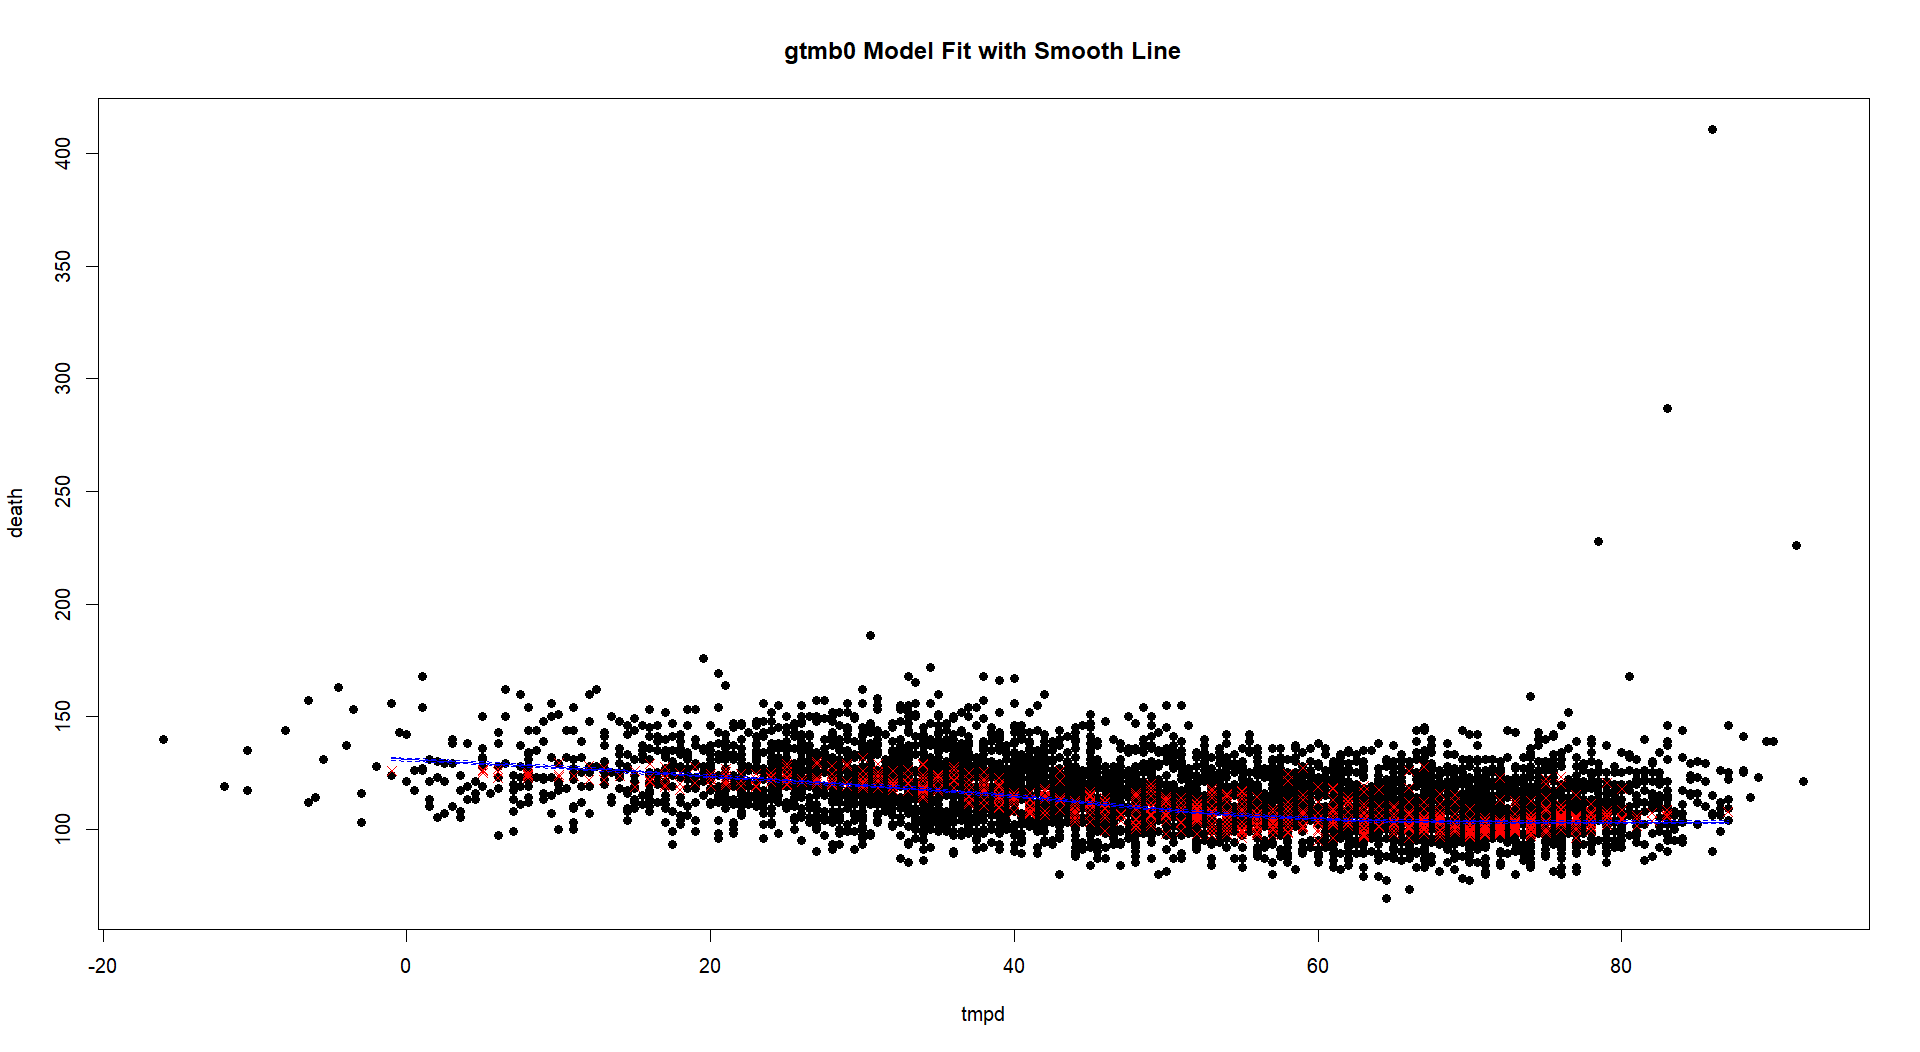
\includegraphics[width=0.9\textwidth]{visuals/Model_fit_gtmb0.png}
    \caption{Model Fit for gtmb0}
    \label{fig:modfit_gtmb0}
\end{figure}

% DHARMa Residuals for gtmb0
\begin{figure}[h]
    \centering
    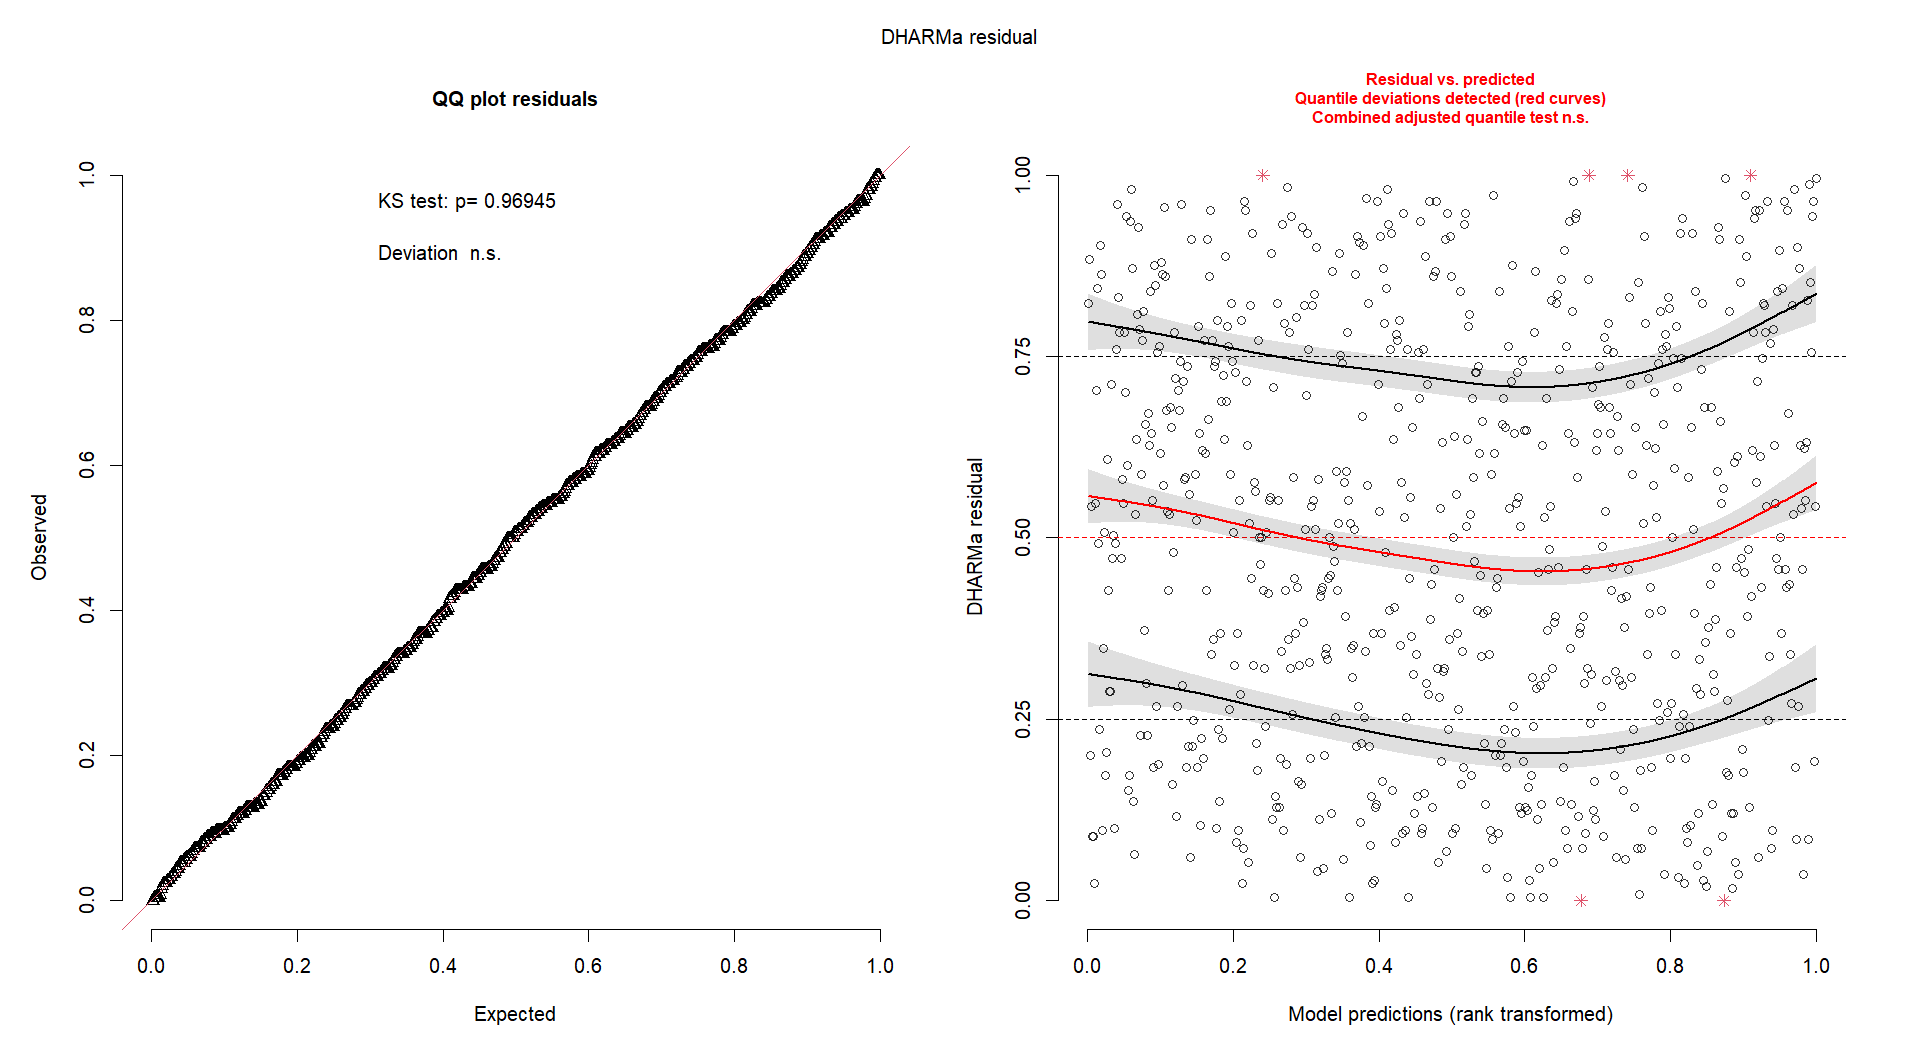
\includegraphics[width=0.9\textwidth]{visuals/DHARMa_gtmb0.png}
    \caption{DHARMa Residuals for gtmb0}
    \label{fig:dharmagtmb0}
\end{figure}

% Residual Histogram for gtmb0
\begin{figure}[h]
    \centering
    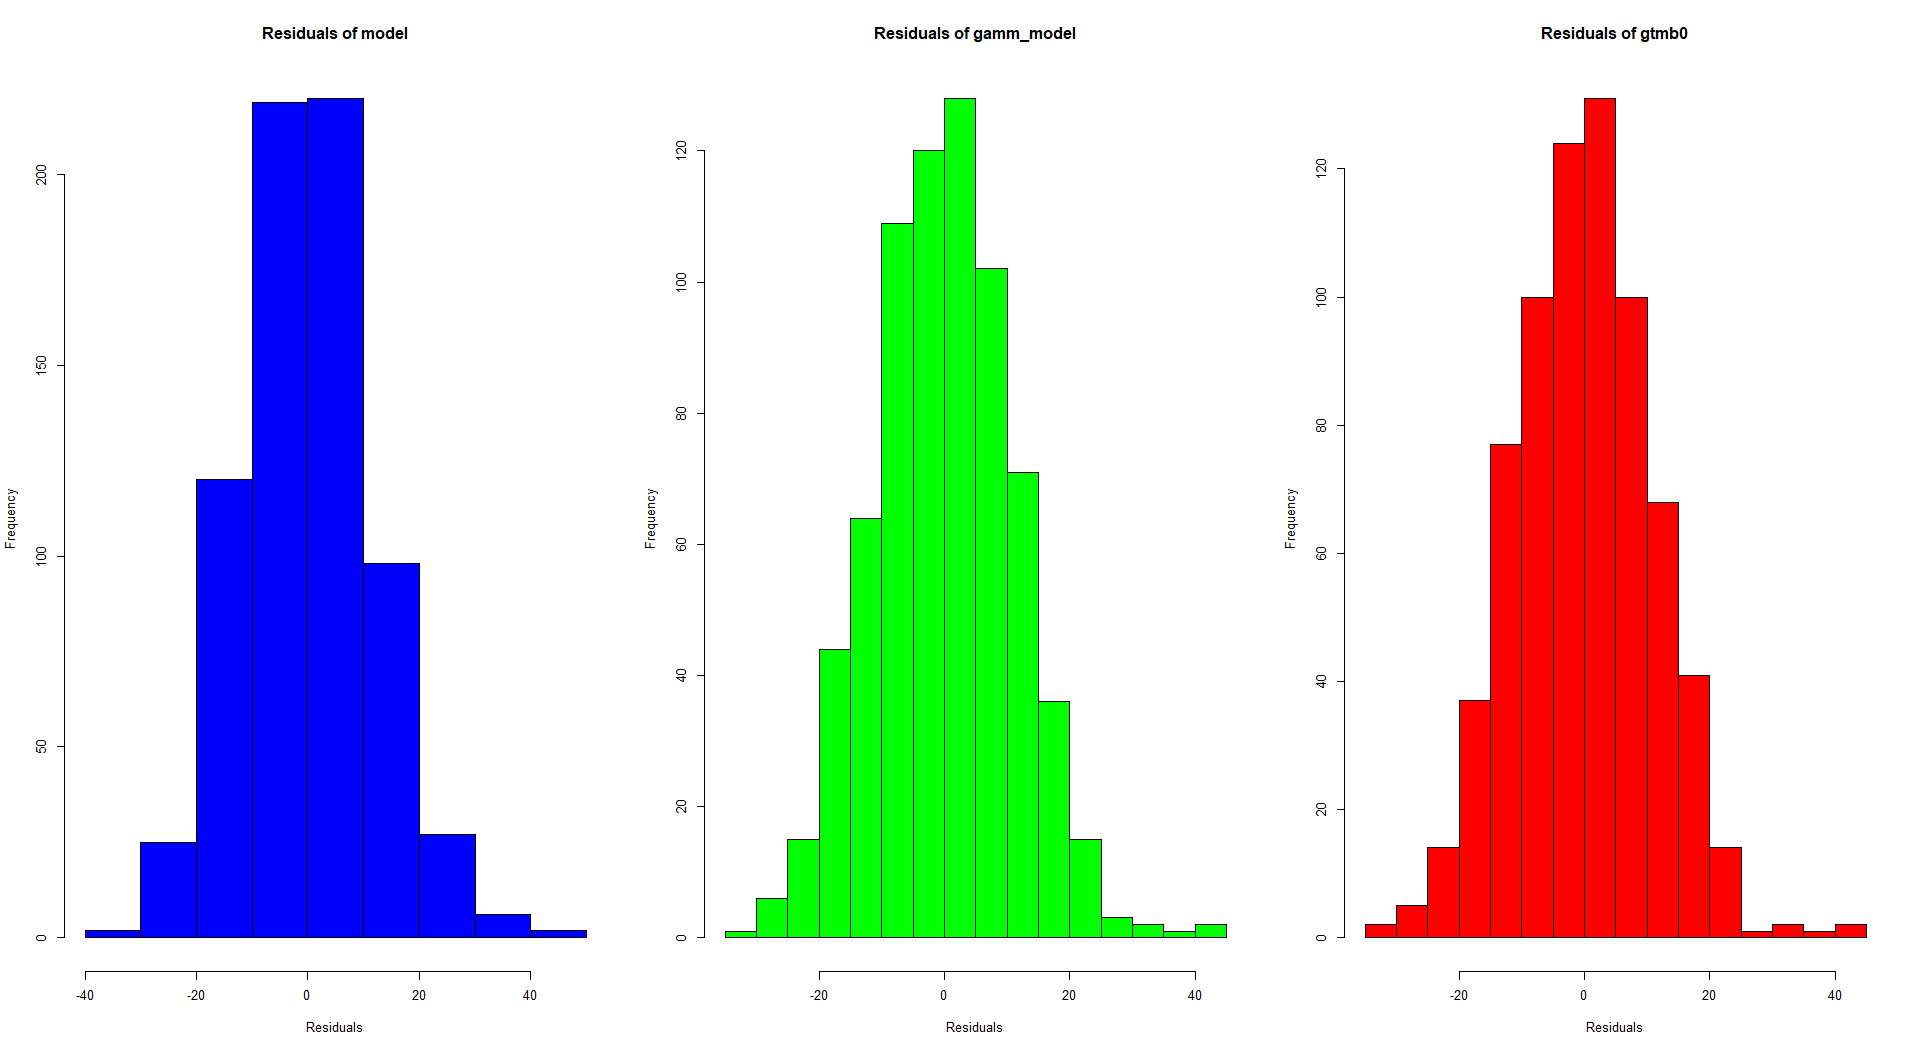
\includegraphics[width=0.9\textwidth]{visuals/residialhist_0.png}
    \caption{Residual Histogram for gtmb0}
    \label{fig:residhist0}
\end{figure}

% Comparison of Histograms for Model 0
\begin{figure}[h]
    \centering
    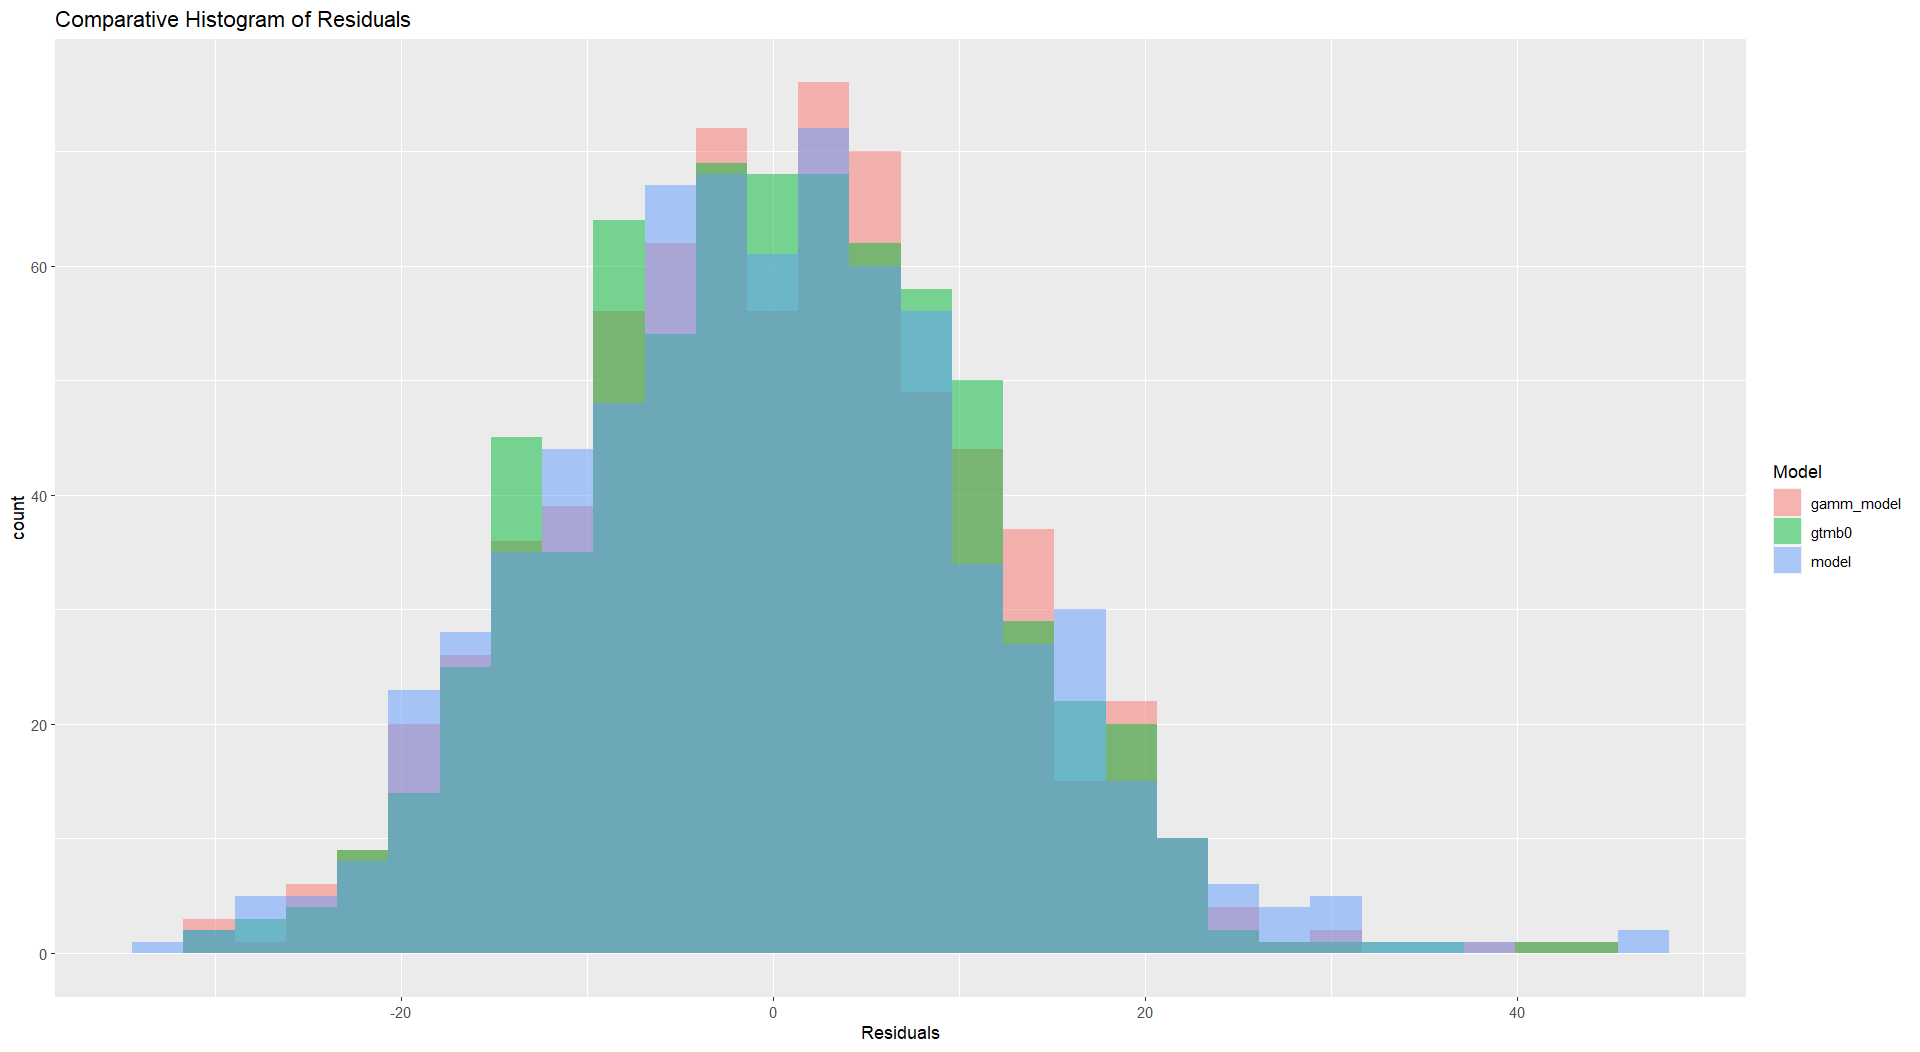
\includegraphics[width=0.9\textwidth]{visuals/comparehists_0.png}
    \caption{Comparison of Histograms for Model 0}
    \label{fig:comparehists0}
\end{figure}

% DHARMa Residuals for gmbt1
\begin{figure}[h]
    \centering
    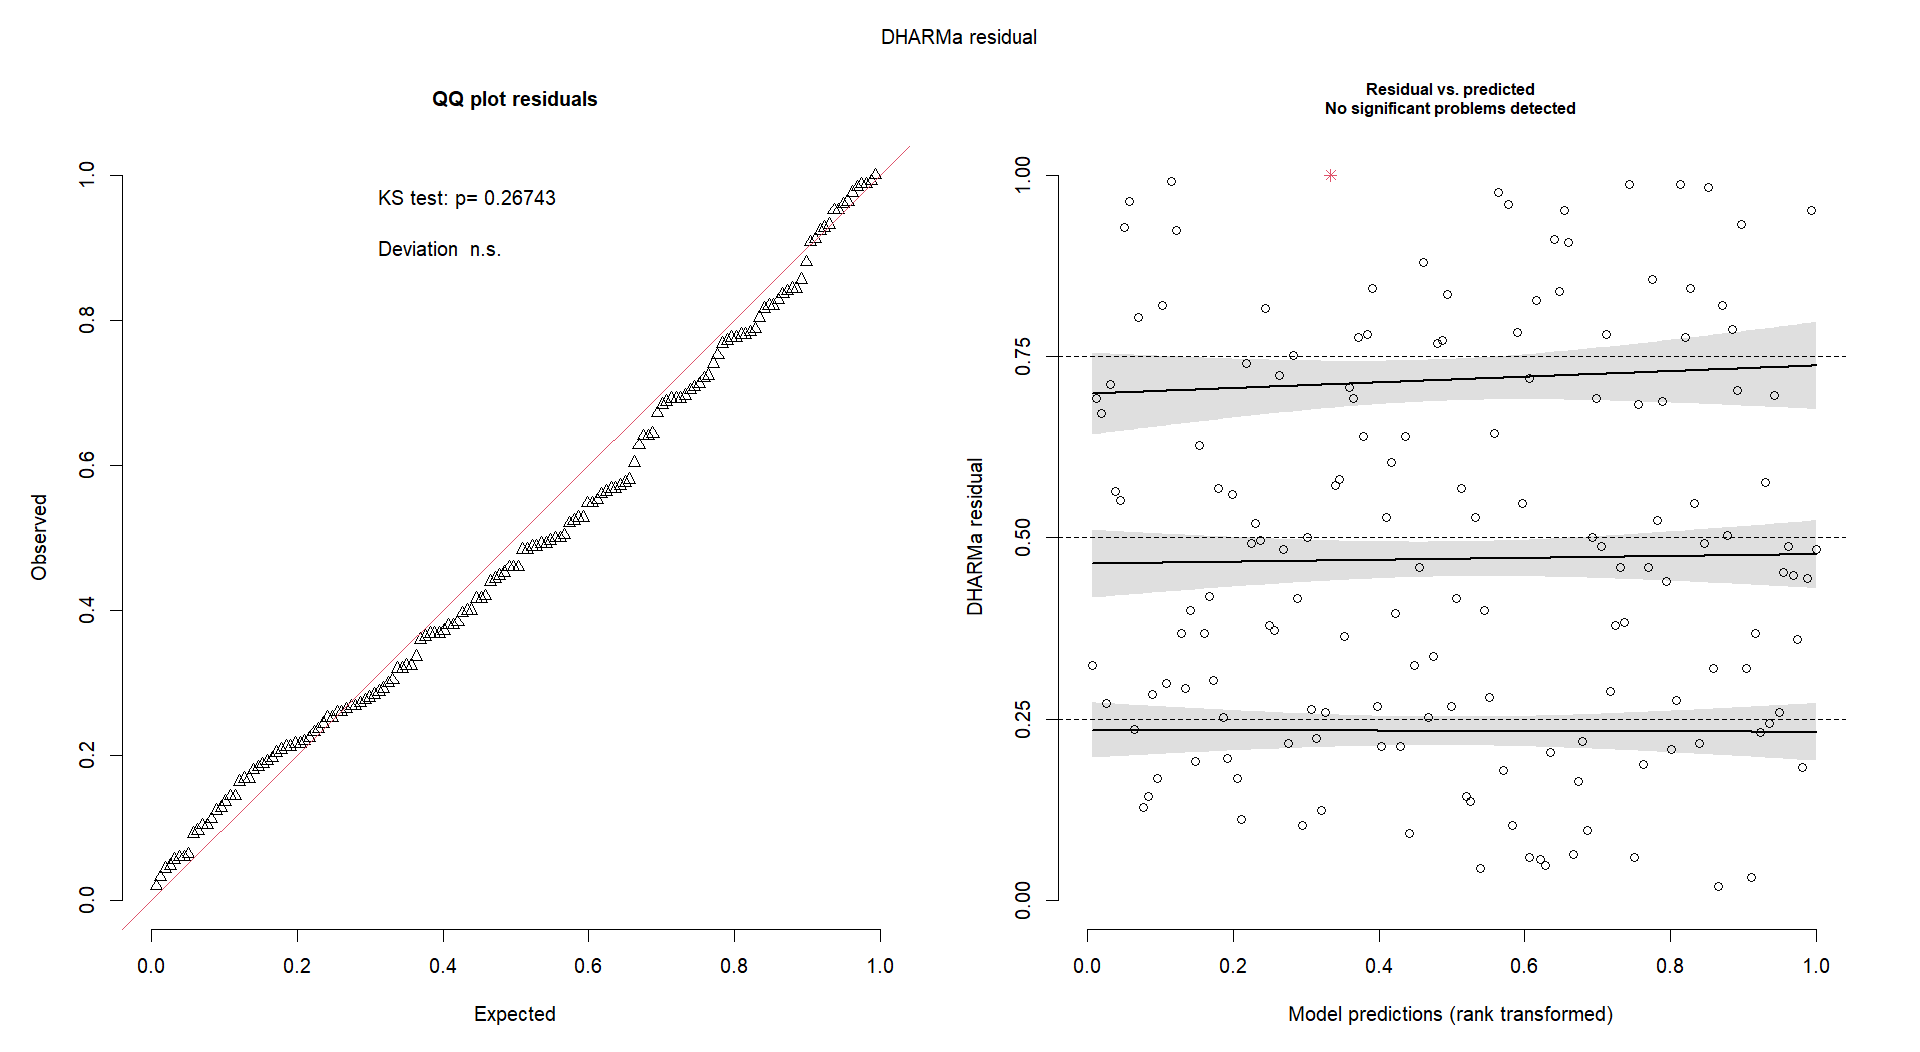
\includegraphics[width=0.9\textwidth]{visuals/DHARMa_gmbt1.png}
    \caption{DHARMa Residuals for gmbt1}
    \label{fig:dharmagmbt1}
\end{figure}

% DHARMa Residuals for gam1
\begin{figure}[h]
    \centering
    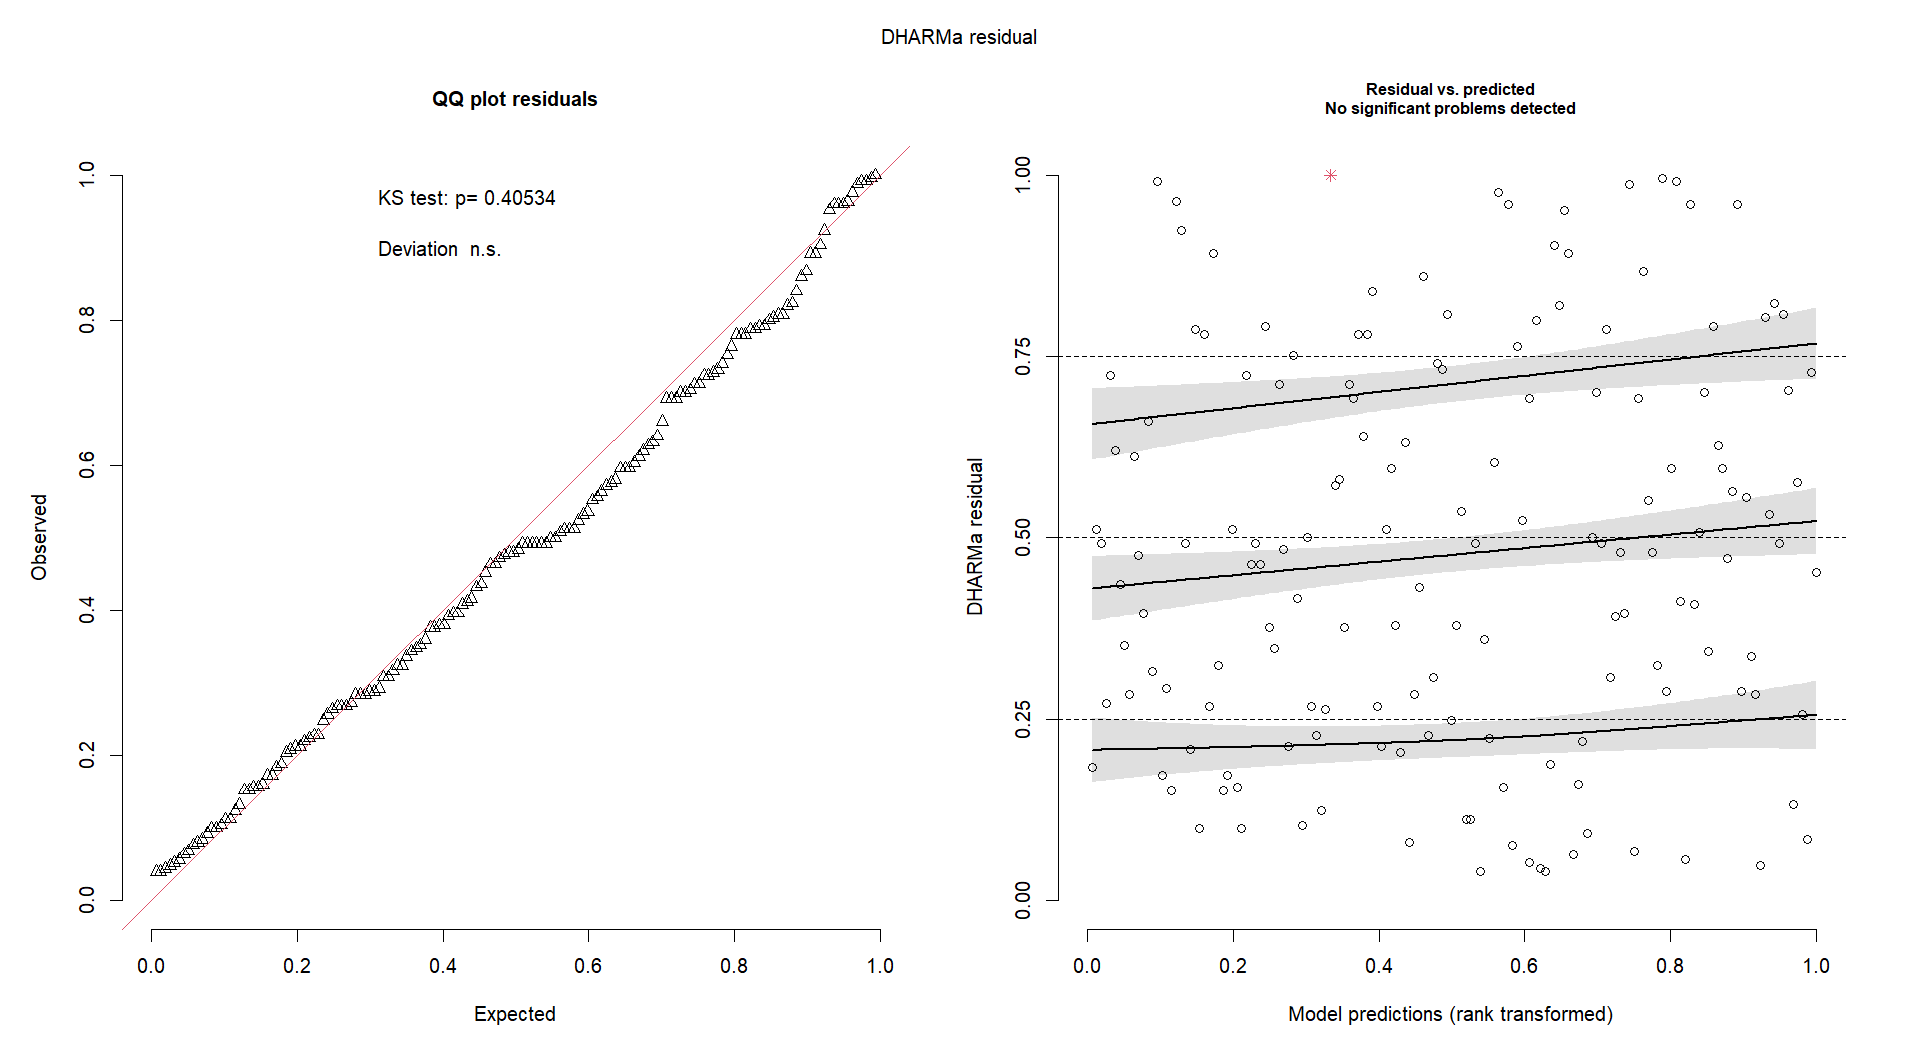
\includegraphics[width=0.9\textwidth]{visuals/DHARMa_gam1.png}
    \caption{DHARMa Residuals for gam1}
    \label{fig:dharmagam1}
\end{figure}

% Model Fit for gtmb1
\begin{figure}[h]
    \centering
    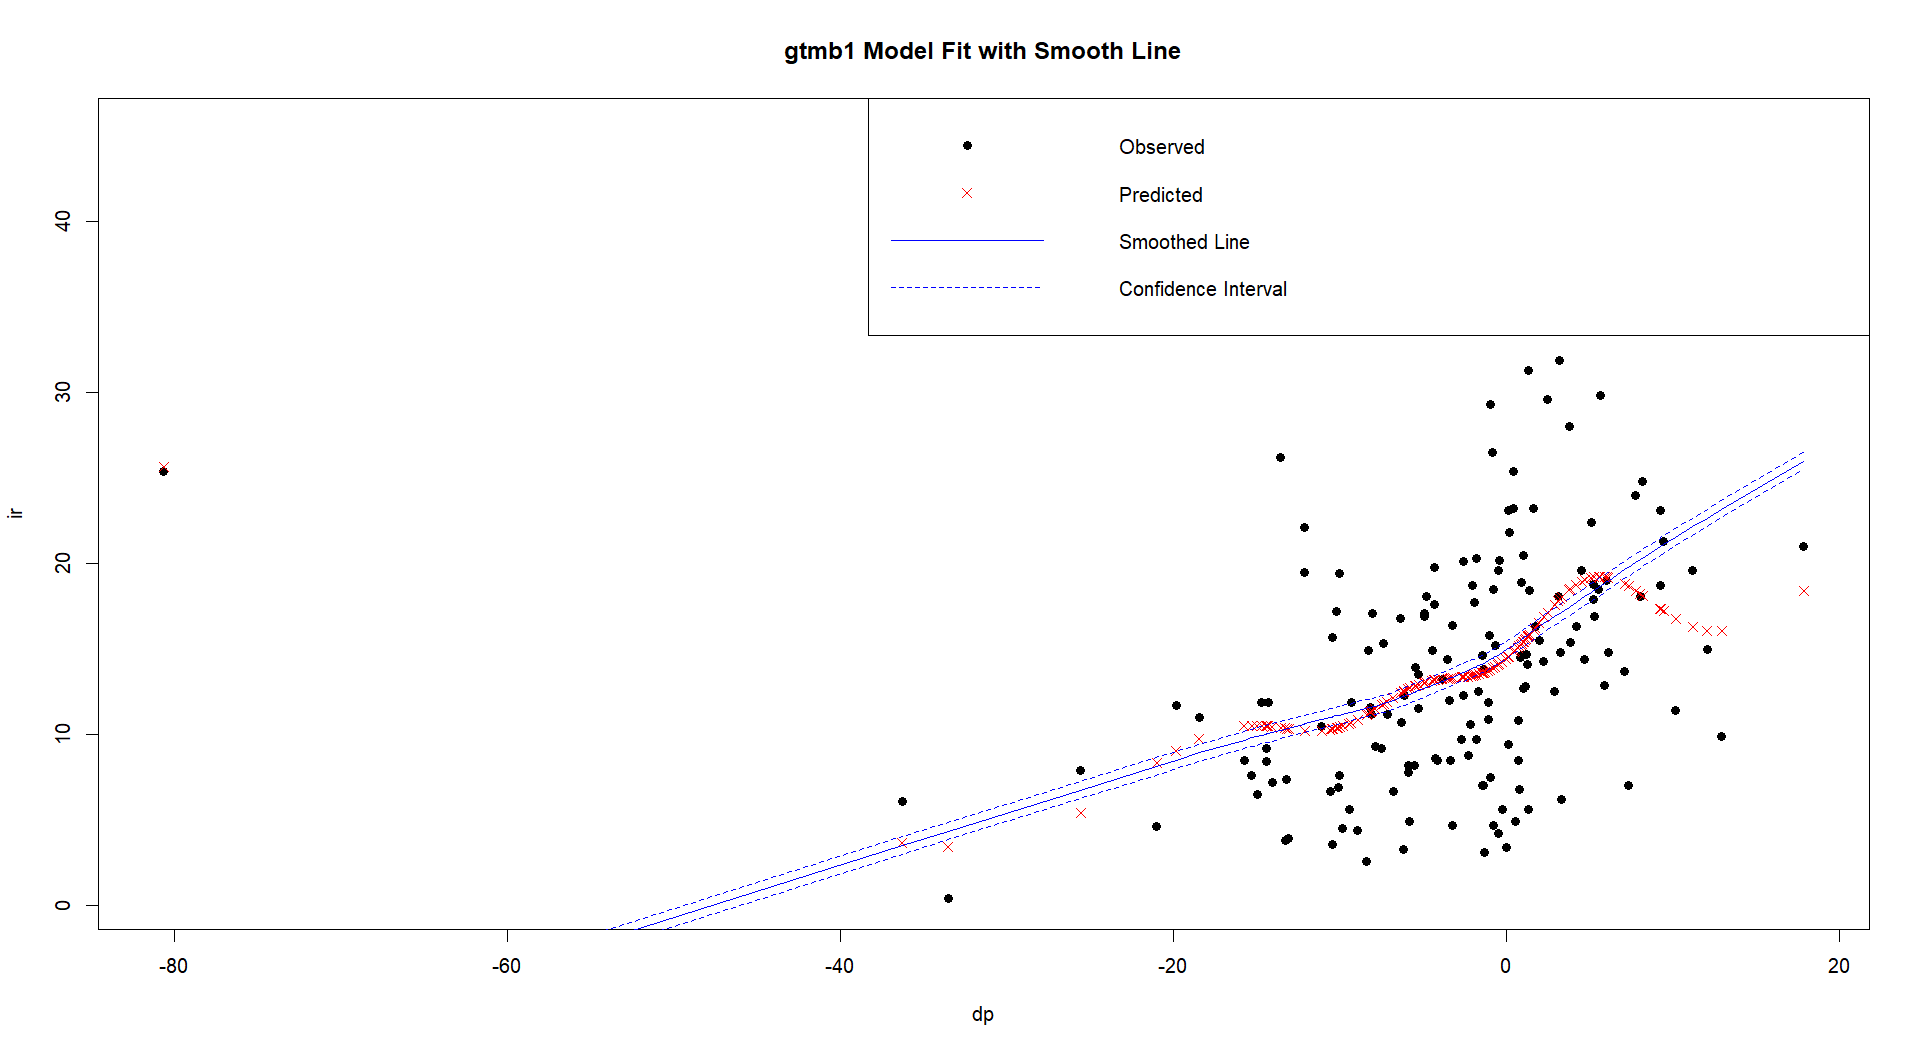
\includegraphics[width=0.9\textwidth]{visuals/modfit_gtmb1.png}
    \caption{Model Fit for gtmb1}
    \label{fig:modfitgtmb1}
\end{figure}

% Model Fit for gtmb1 (Duplicate)
\begin{figure}[h]
    \centering
    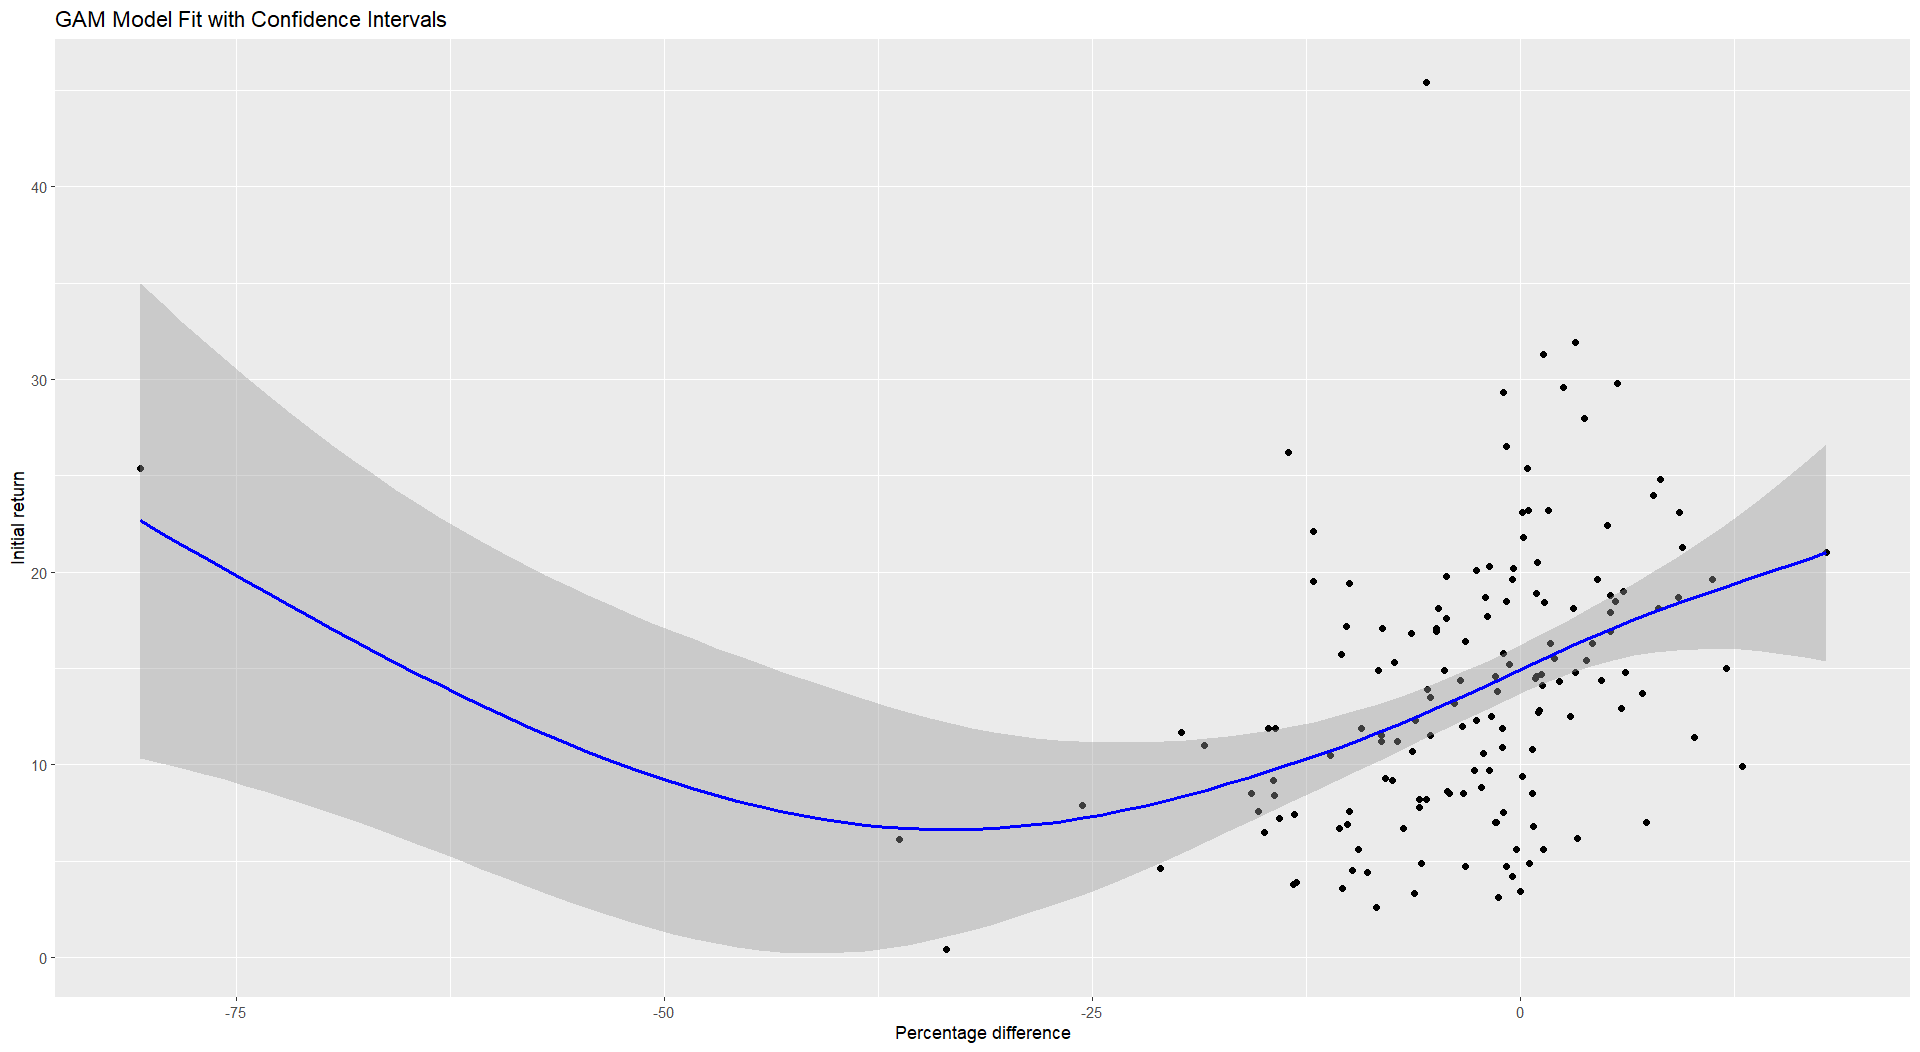
\includegraphics[width=0.9\textwidth]{visuals/modelfit_gam1.png}
    \caption{Model Fit for gam1 }
    \label{fig:modfitgtmb1}
\end{figure}

% Residual Histograms for Model 1
\begin{figure}[h]
    \centering
    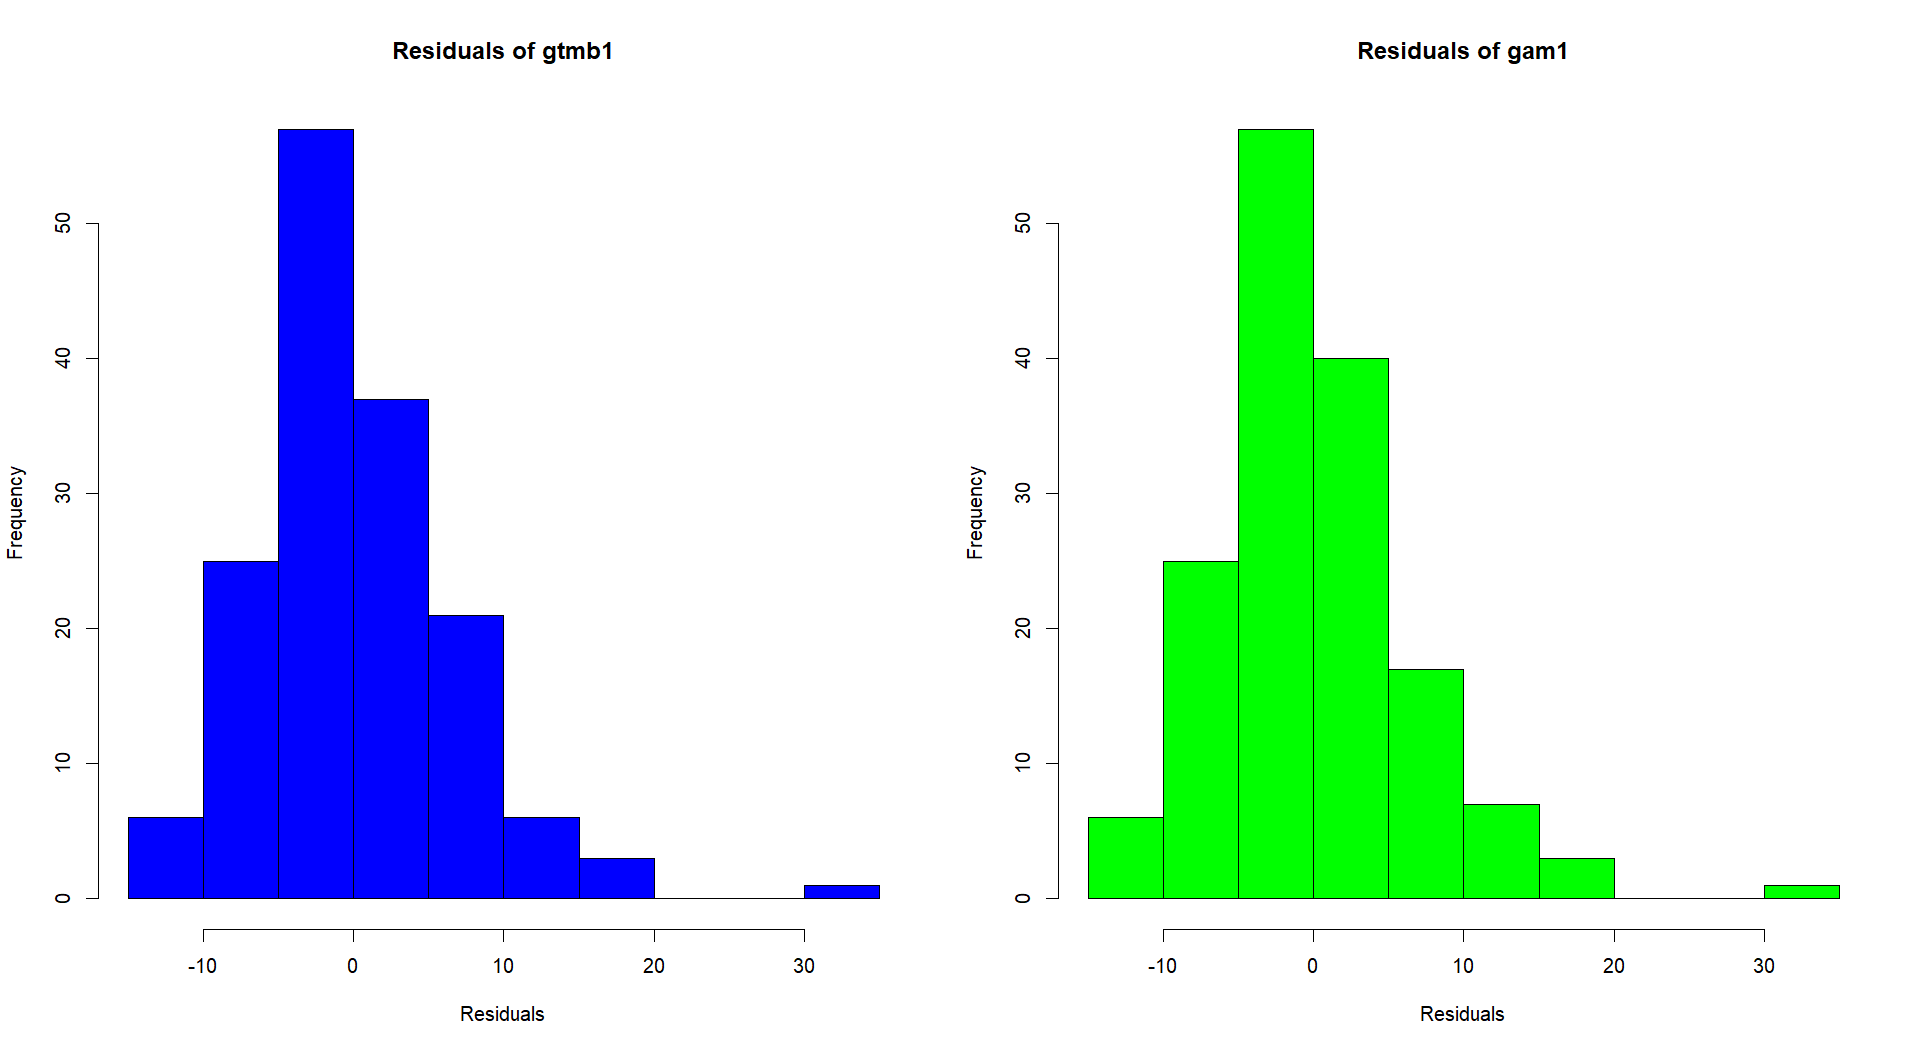
\includegraphics[width=0.9\textwidth]{visuals/residualhists_1.png}
    \caption{Residual Histograms for Model 1}
    \label{fig:residualhists1}
\end{figure}

% DHARMa Residuals for gtmb2
\begin{figure}[h]
    \centering
    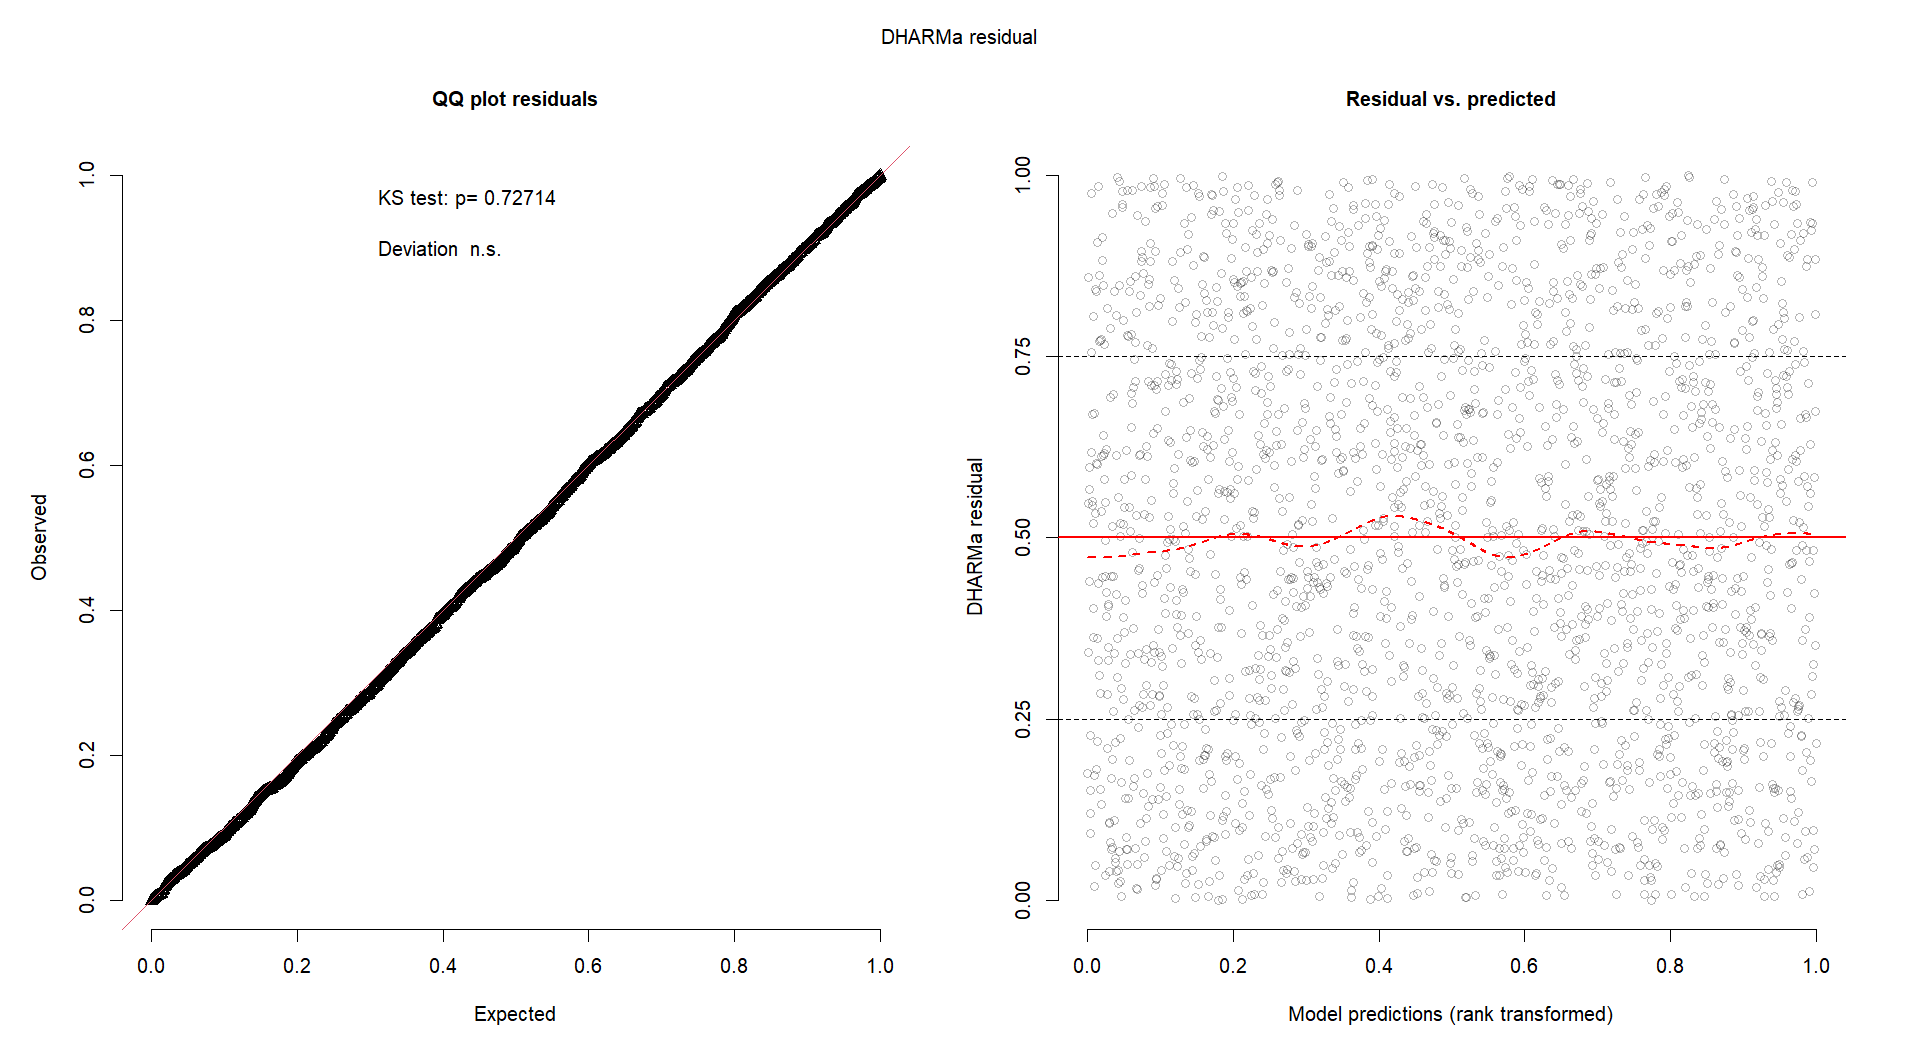
\includegraphics[width=0.9\textwidth]{visuals/DHARMa_gtmb2.png}
    \caption{DHARMa Residuals for gtmb2}
    \label{fig:dharmagtmb2}
\end{figure}

% DHARMa Residuals for gam2
\begin{figure}[h]
    \centering
    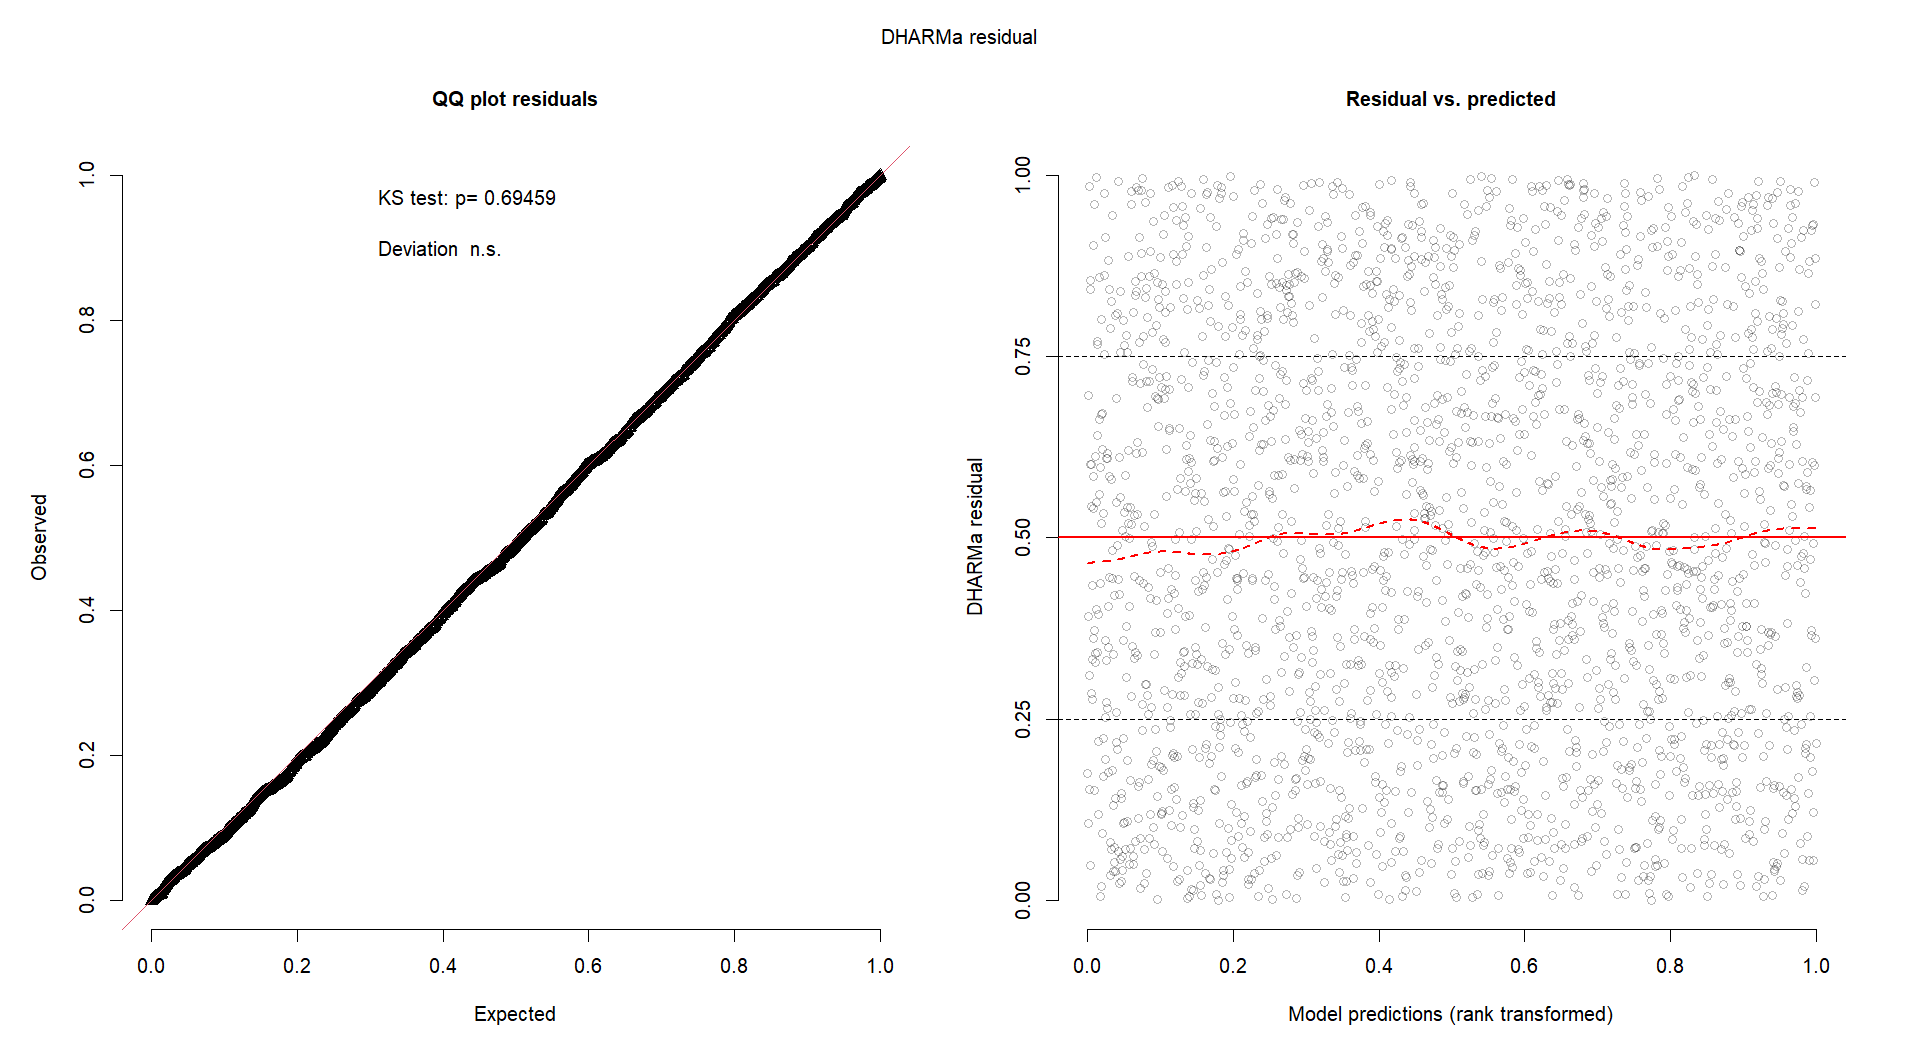
\includegraphics[width=0.9\textwidth]{visuals/DHARMa_gam2.png}
    \caption{DHARMa Residuals for gam2}
    \label{fig:dharmagam2}
\end{figure}

% Residual Histograms for Model 2
\begin{figure}[h]
    \centering
    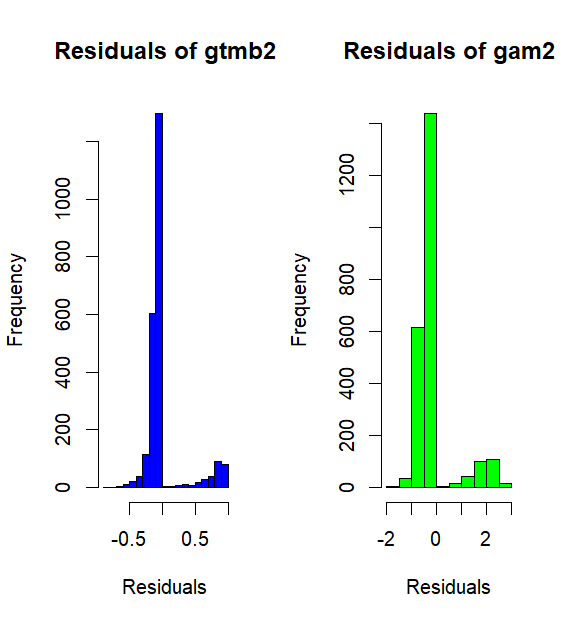
\includegraphics[width=0.9\textwidth]{visuals/reidualshists_2.png}
    \caption{Residual Histograms for Model 2}
    \label{fig:residualhists2}
\end{figure}

% AUC Plot
\begin{figure}[h]
    \centering
    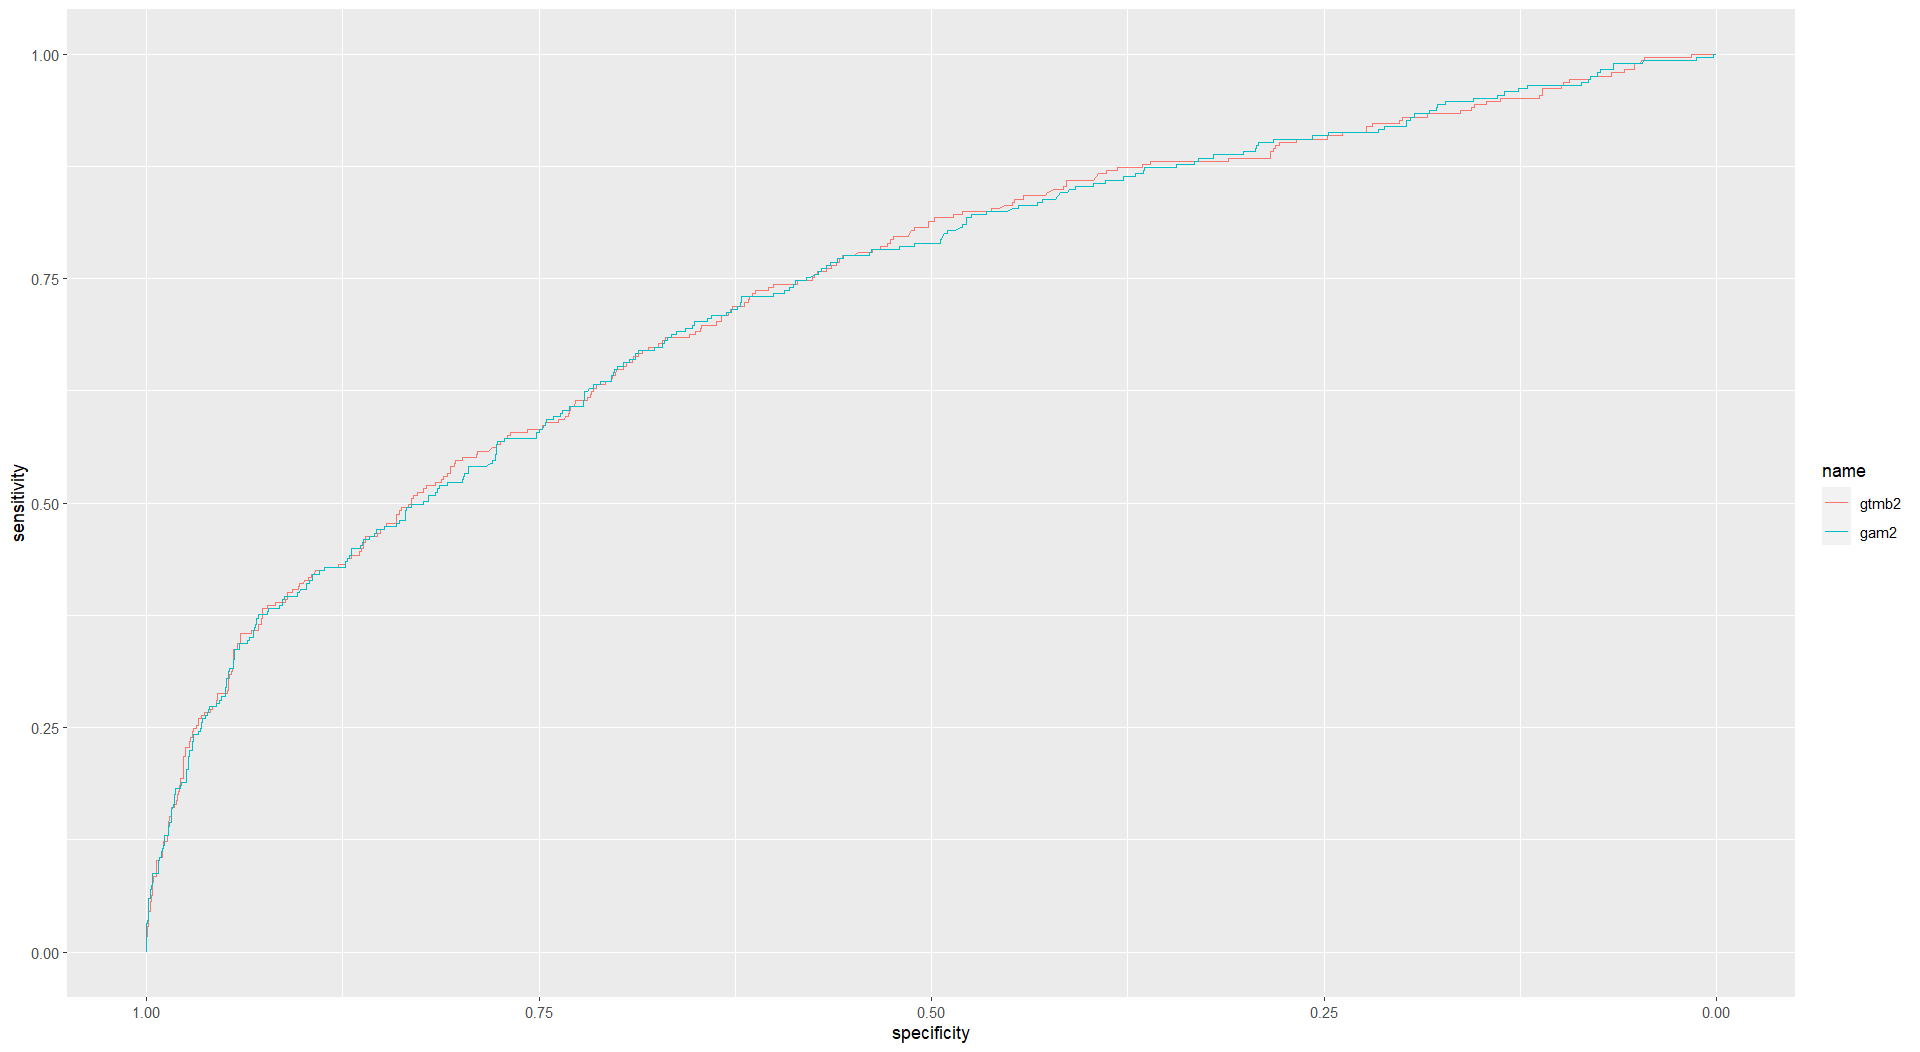
\includegraphics[width=0.9\textwidth]{visuals/AUCplot.png}
    \caption{AUC Plot}
    \label{fig:aucplot}
\end{figure}

% DHARMa Residuals for gam3
\begin{figure}[h]
    \centering
    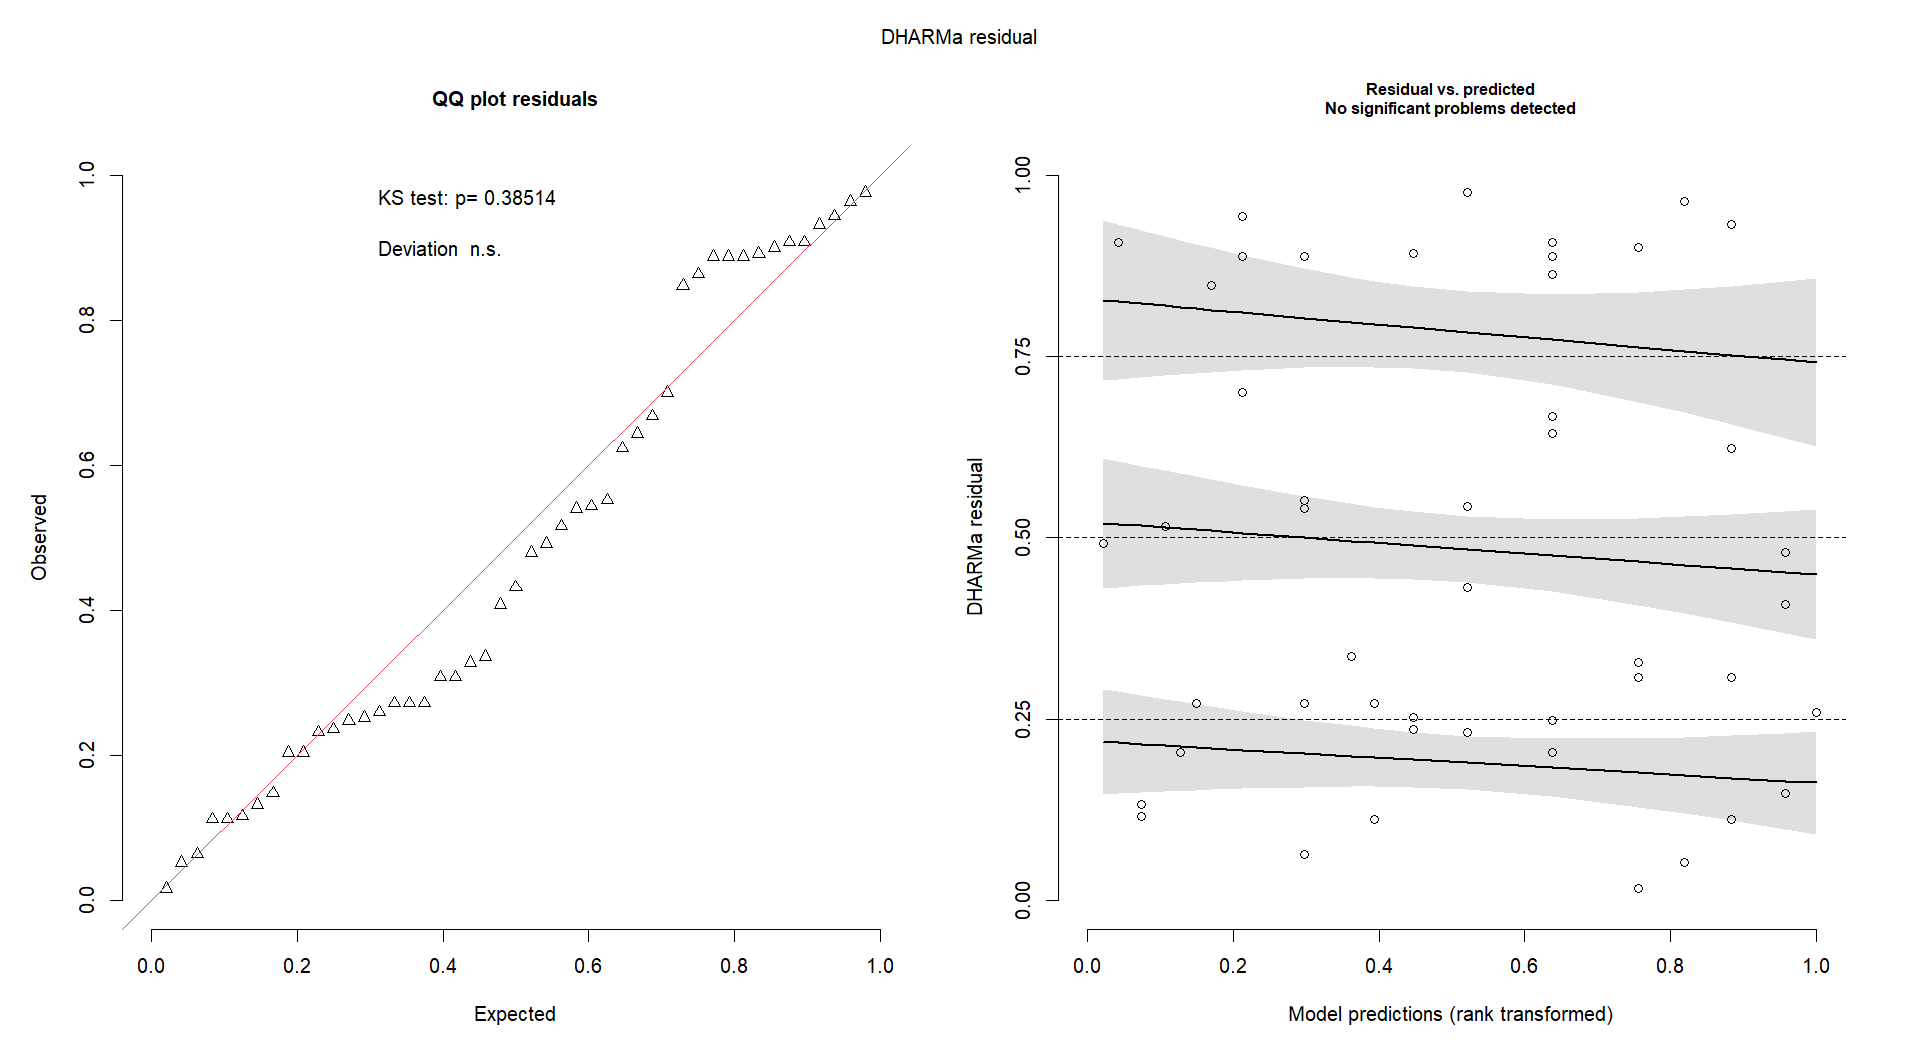
\includegraphics[width=0.9\textwidth]{visuals/DHARMa_gam3.png}
    \caption{DHARMa Residuals for gam3}
    \label{fig:dharmagam3}
\end{figure}

% DHARMa Residuals for gtmb3
\begin{figure}[h]
    \centering
    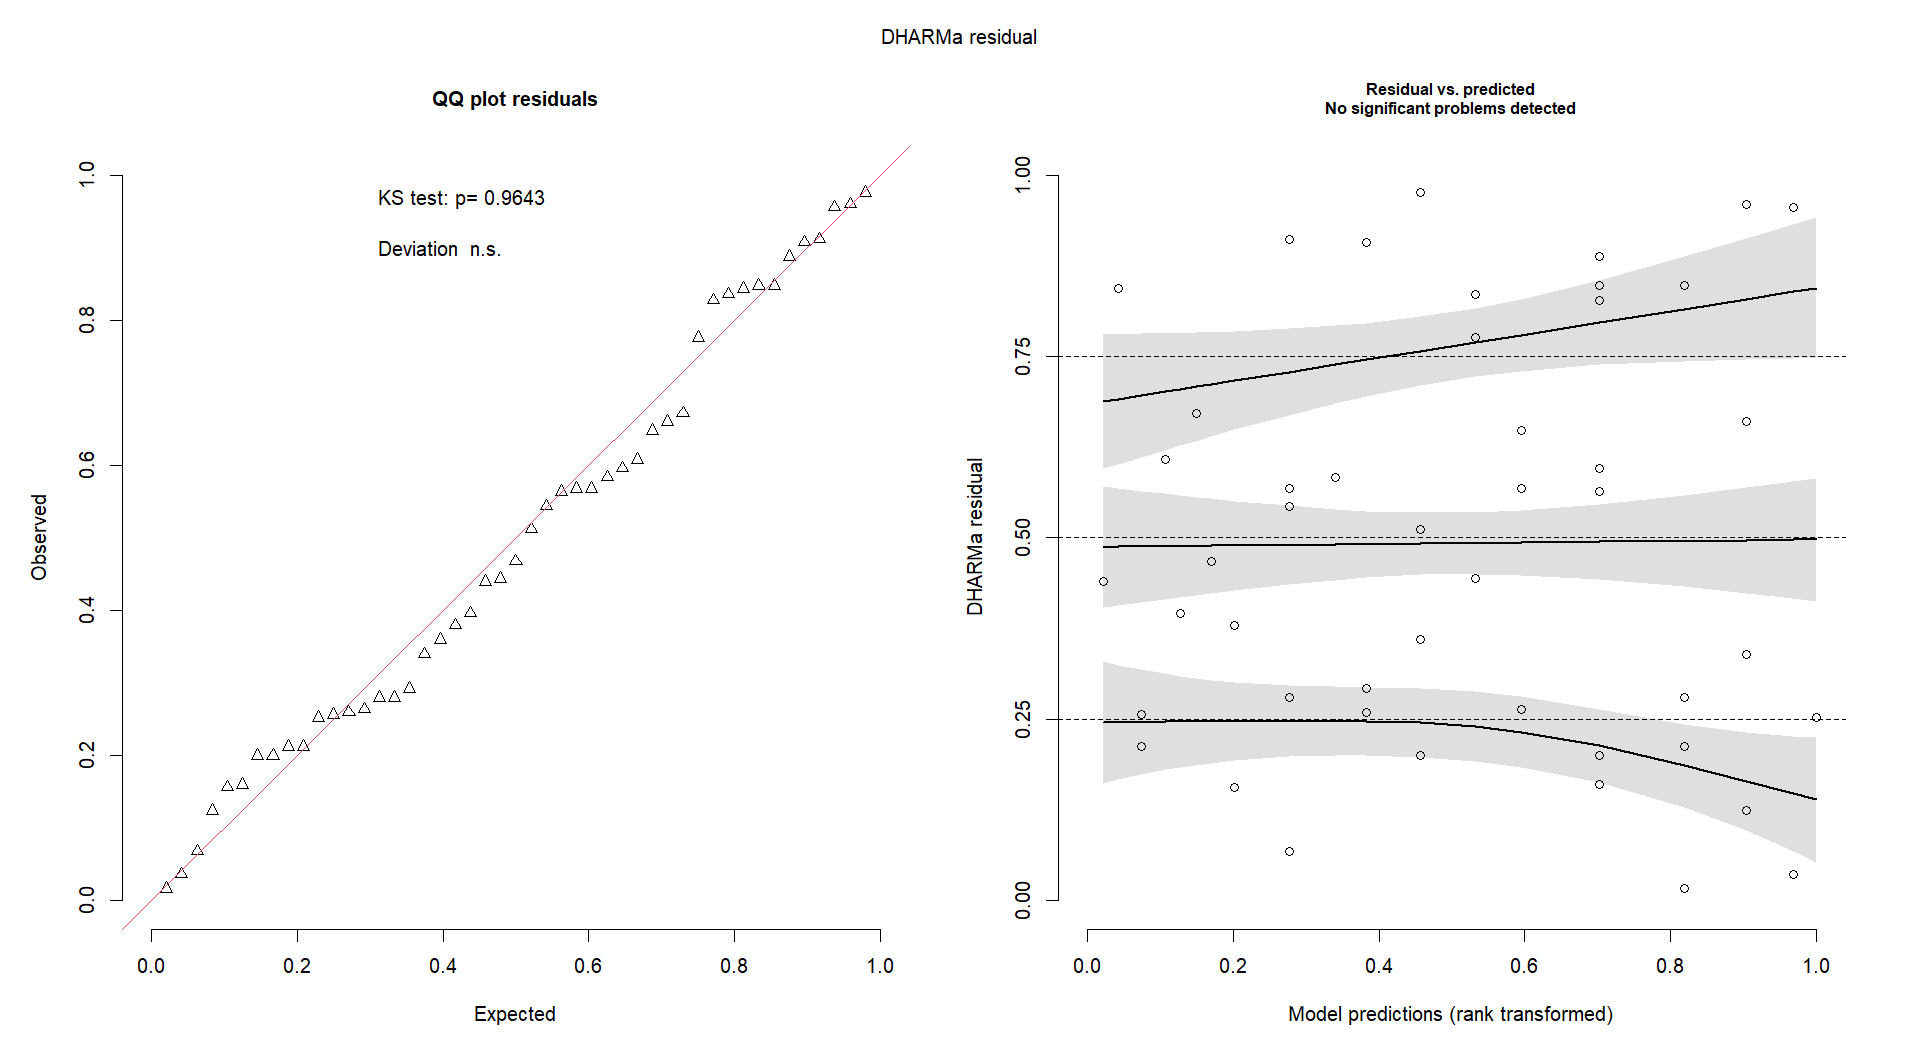
\includegraphics[width=0.9\textwidth]{visuals/DHARMa_gtmb3.png}
    \caption{DHARMa Residuals for gtmb3}
    \label{fig:dharmagtmb3}
\end{figure}

% Model Fit for gtmb3
\begin{figure}[h]
    \centering
    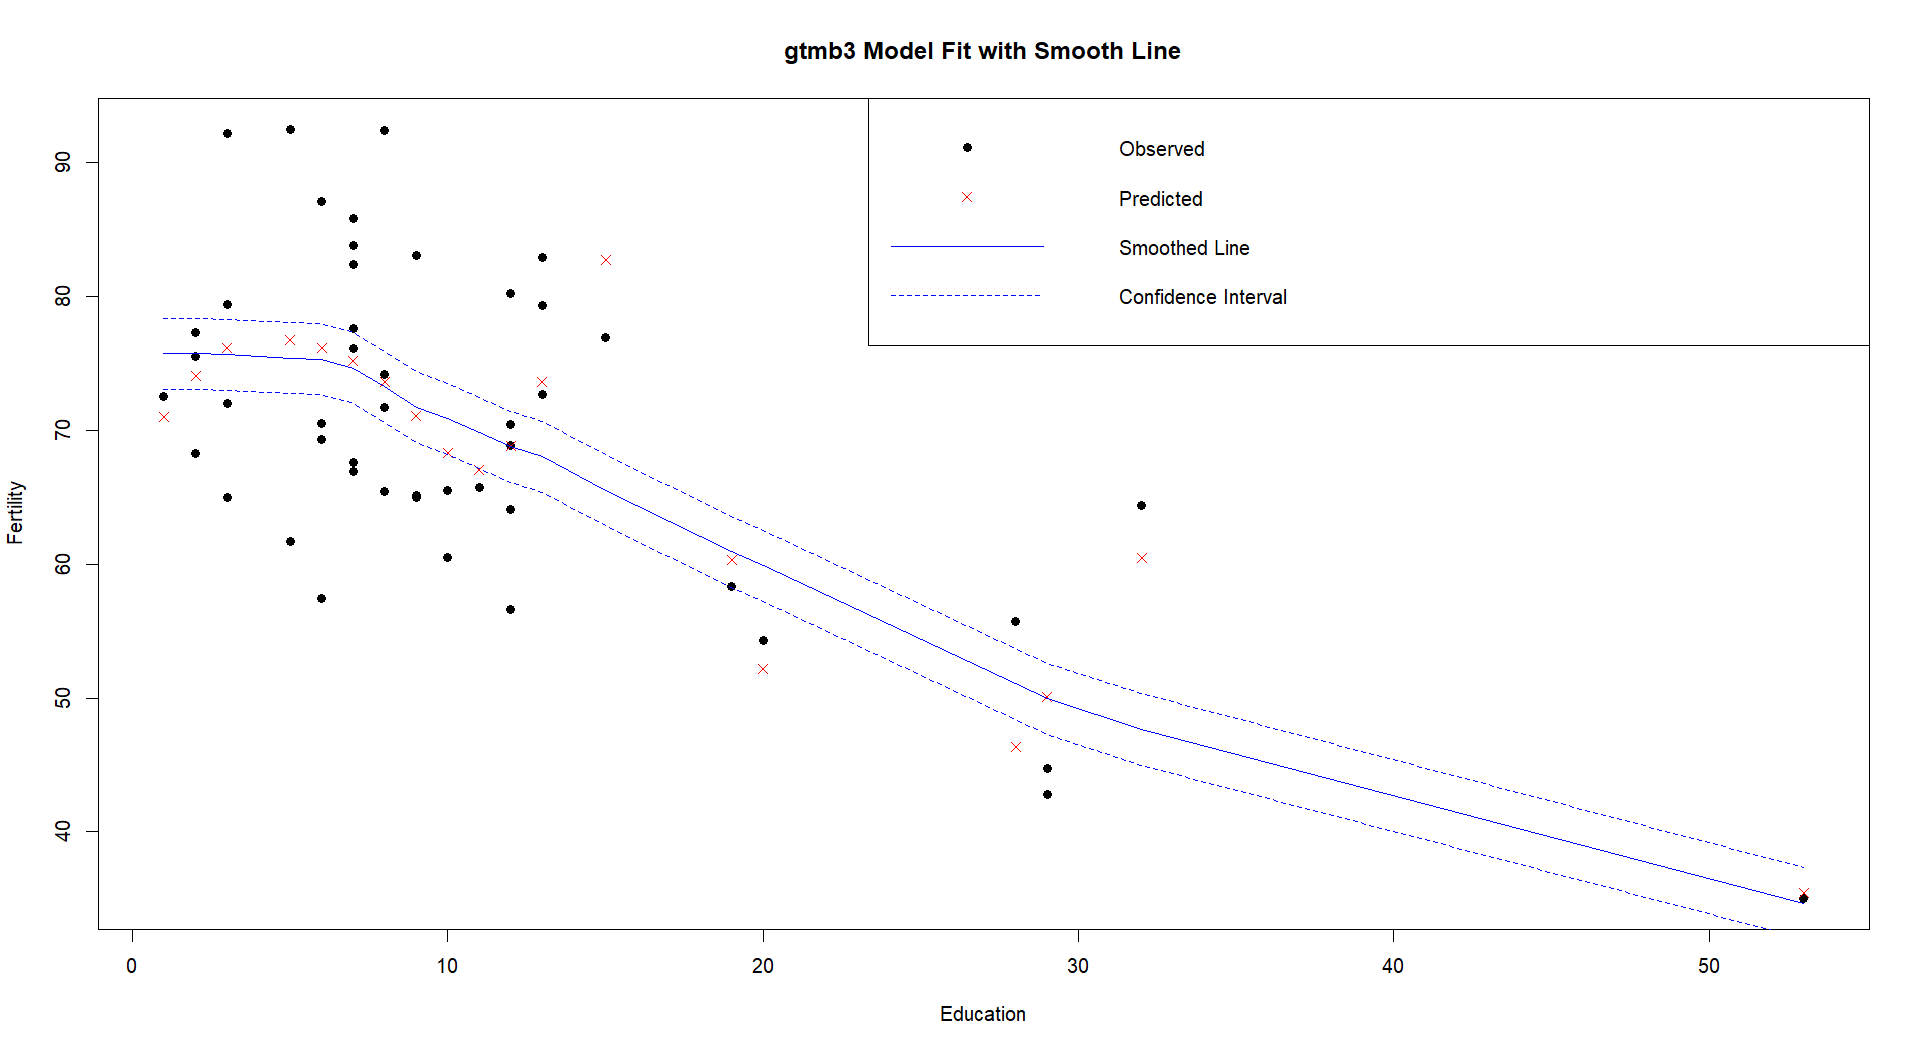
\includegraphics[width=0.9\textwidth]{visuals/model_fit_gtmb3.png}
    \caption{Model Fit for gtmb3}
    \label{fig:modelfitgtmb3}
\end{figure}

% Model Fit for gam3
\begin{figure}[h]
    \centering
    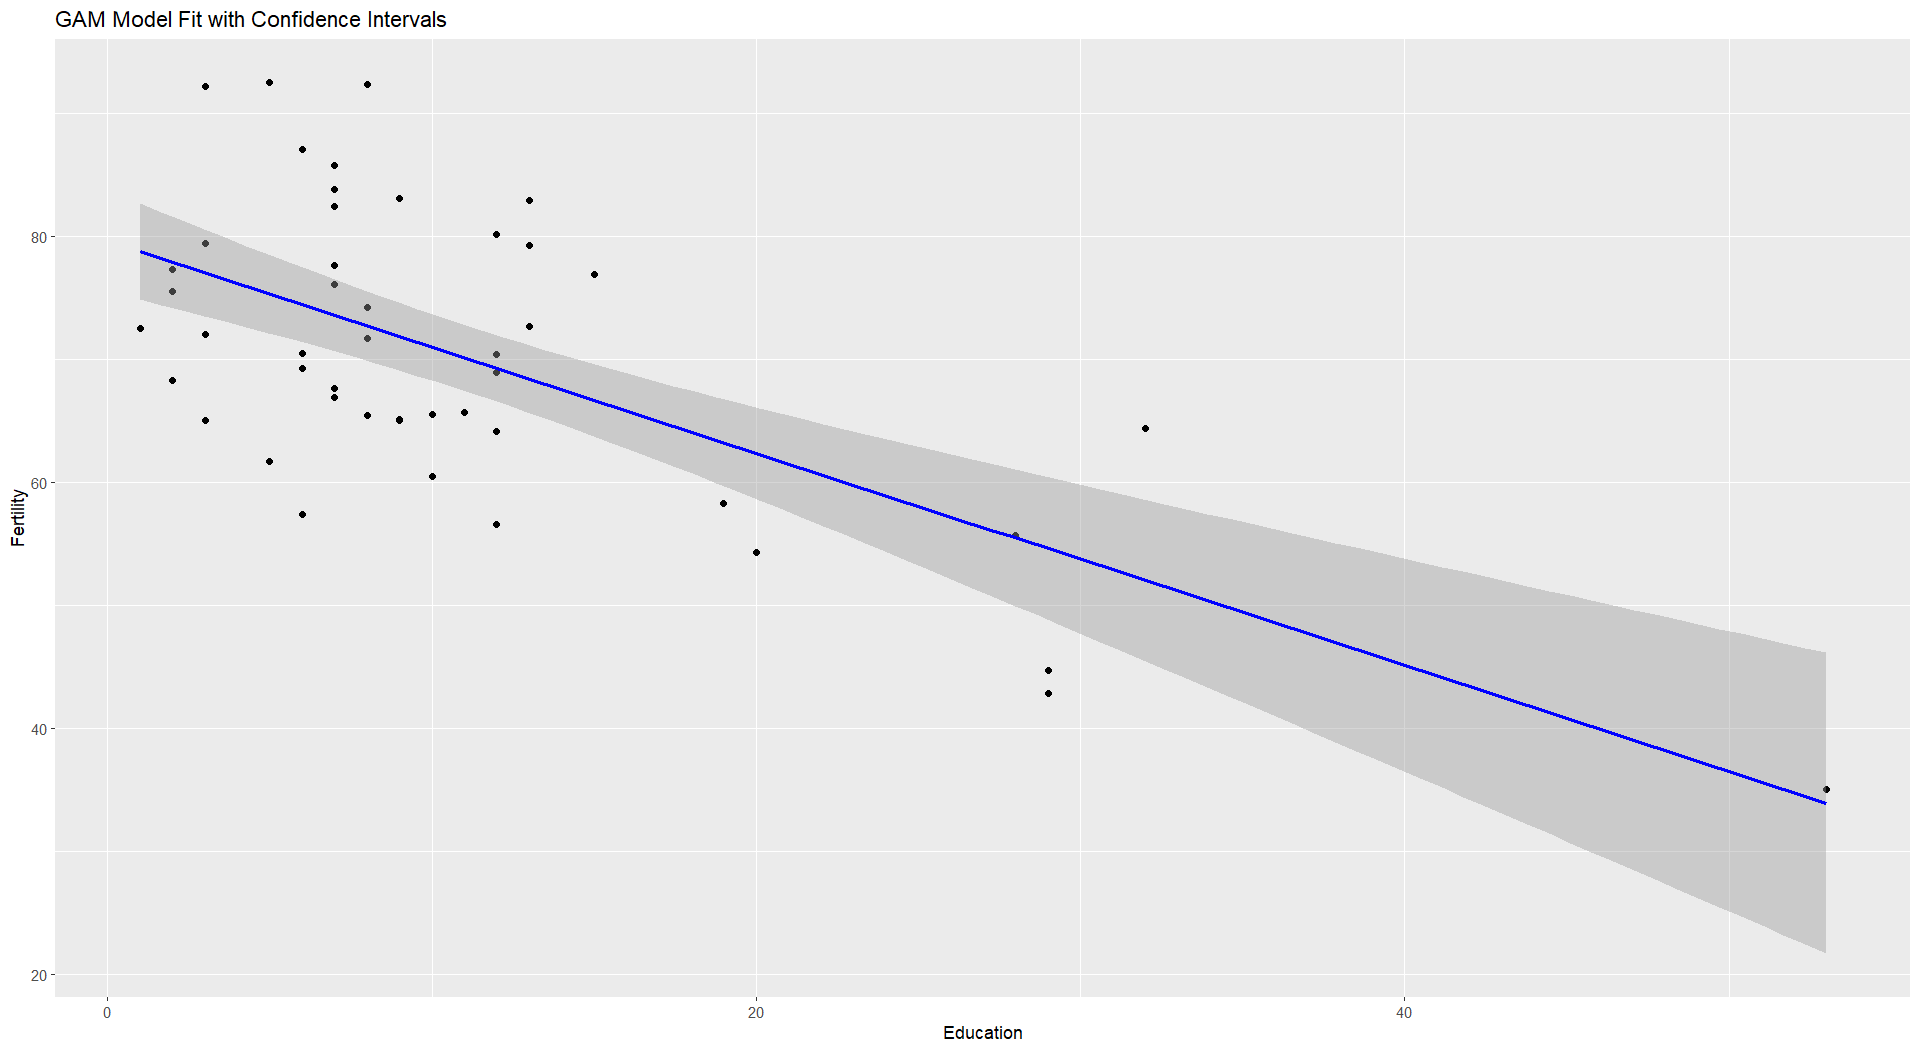
\includegraphics[width=0.9\textwidth]{visuals/model_fit_gam3.png}
    \caption{Model Fit for gam3}
    \label{fig:modelfitgam3}
\end{figure}

% Residuals vs Fit for gtmb3
\begin{figure}[h]
    \centering
    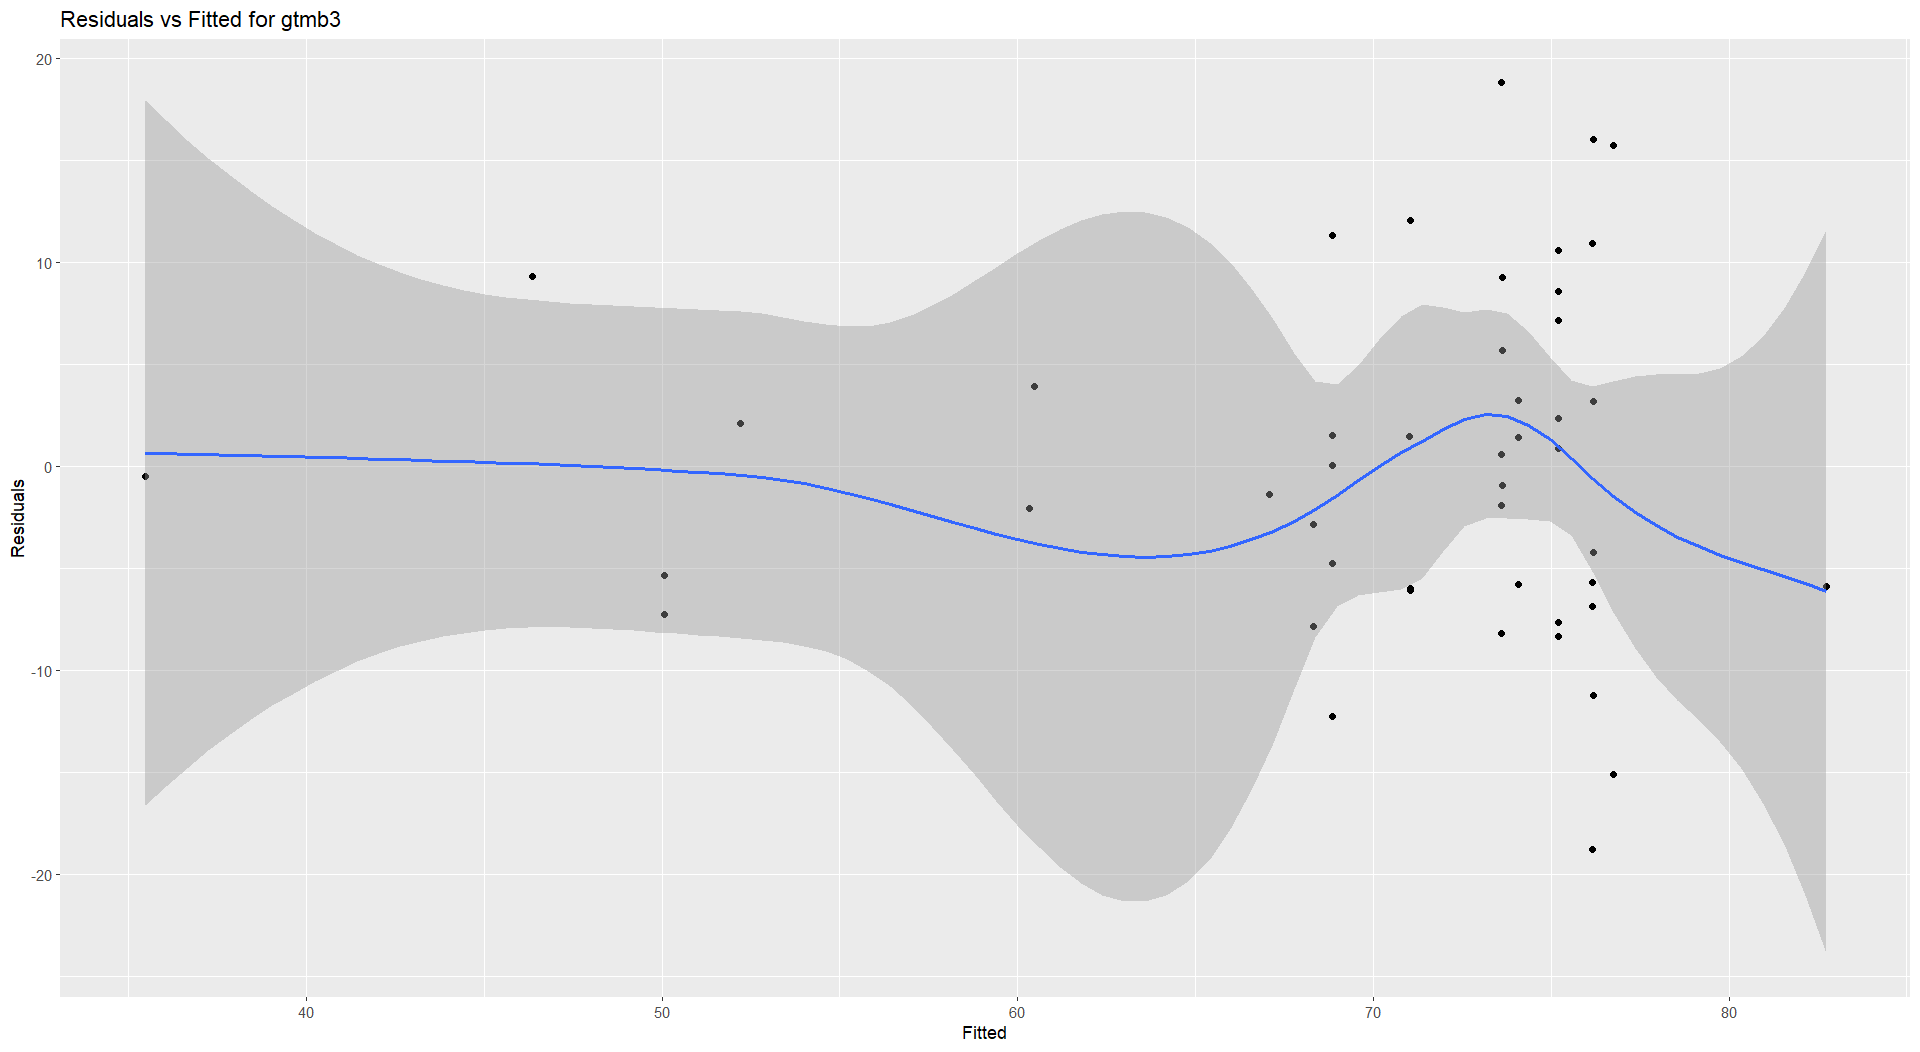
\includegraphics[width=0.9\textwidth]{visuals/resvsfit_gtmb3.png}
    \caption{Residuals vs Fit for gtmb3}
    \label{fig:resvsfitgtmb3}
\end{figure}

% Residuals vs Fit for gam3
\begin{figure}[h]
    \centering
    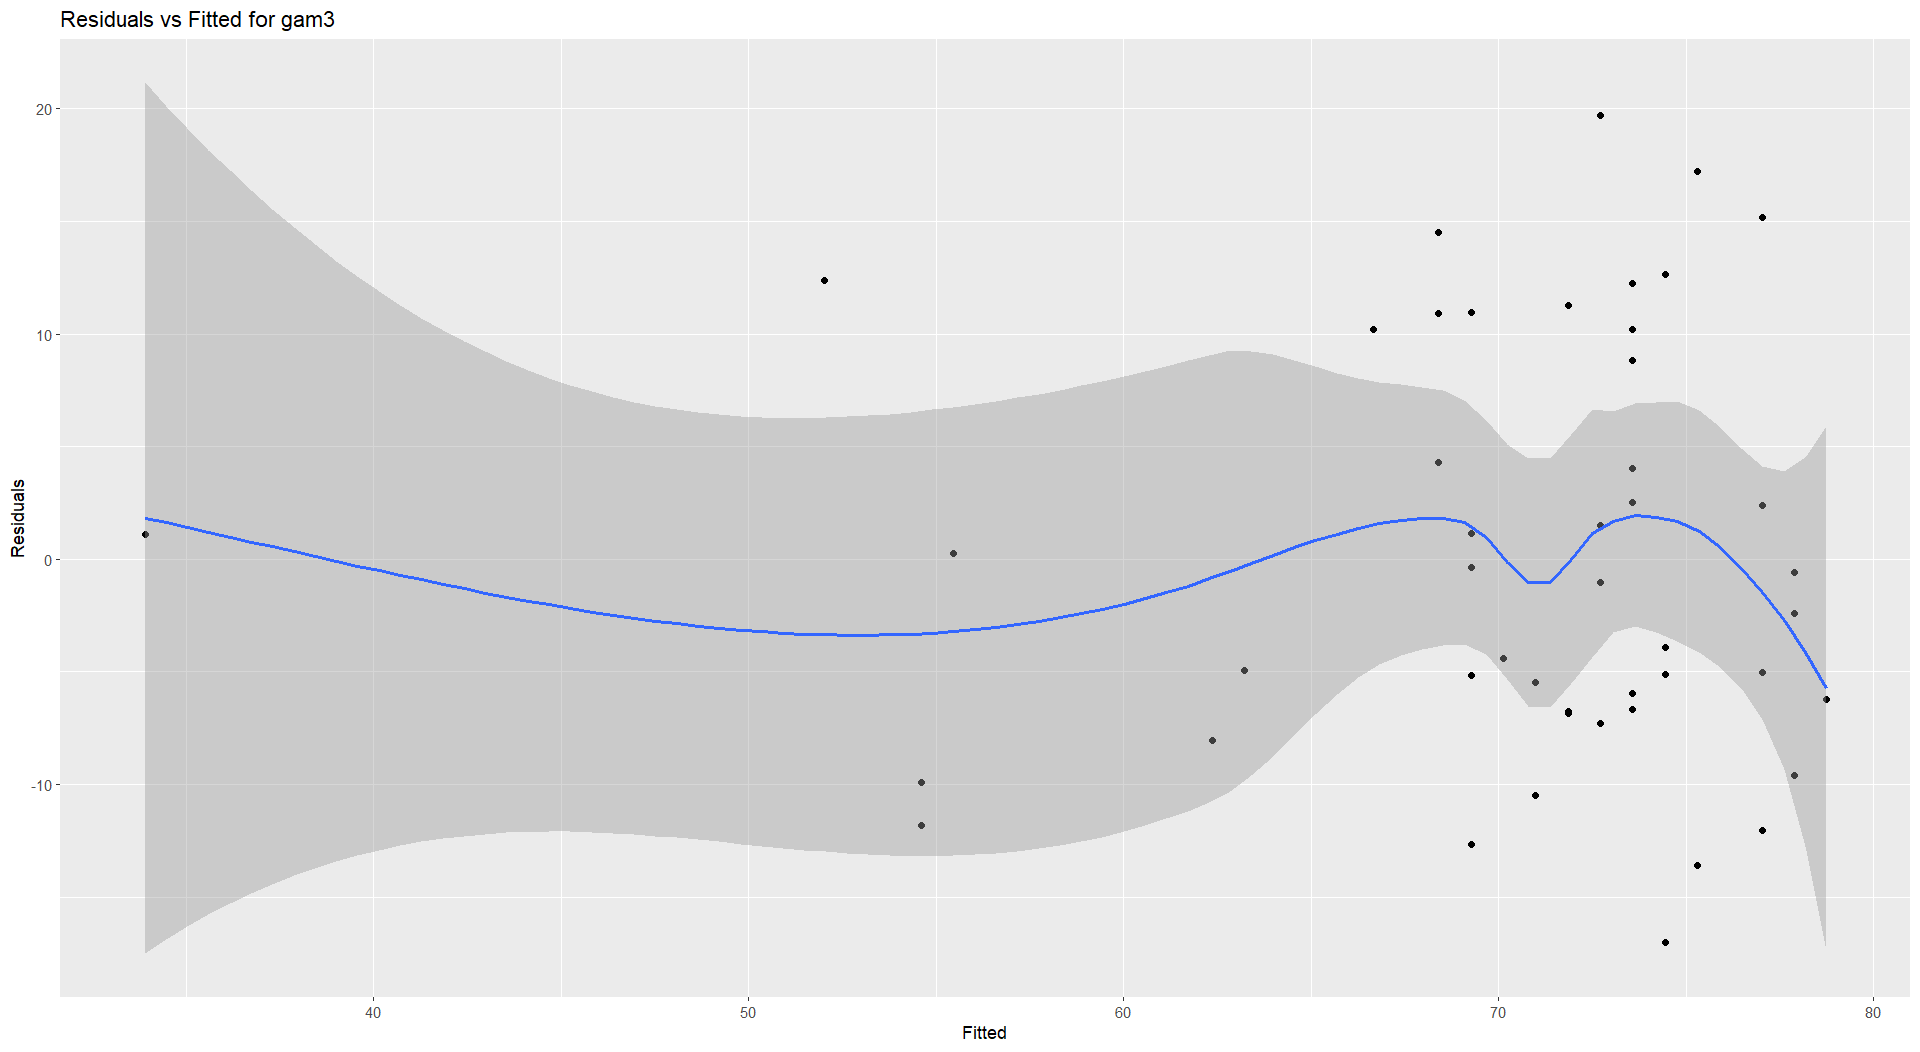
\includegraphics[width=0.9\textwidth]{visuals/resvsfit_gam3.png}
    \caption{Residuals vs Fit for gam3}
    \label{fig:resvsfitgam3}
\end{figure}

% DHARMA for gtmb4
\begin{figure}[h]
    \centering
    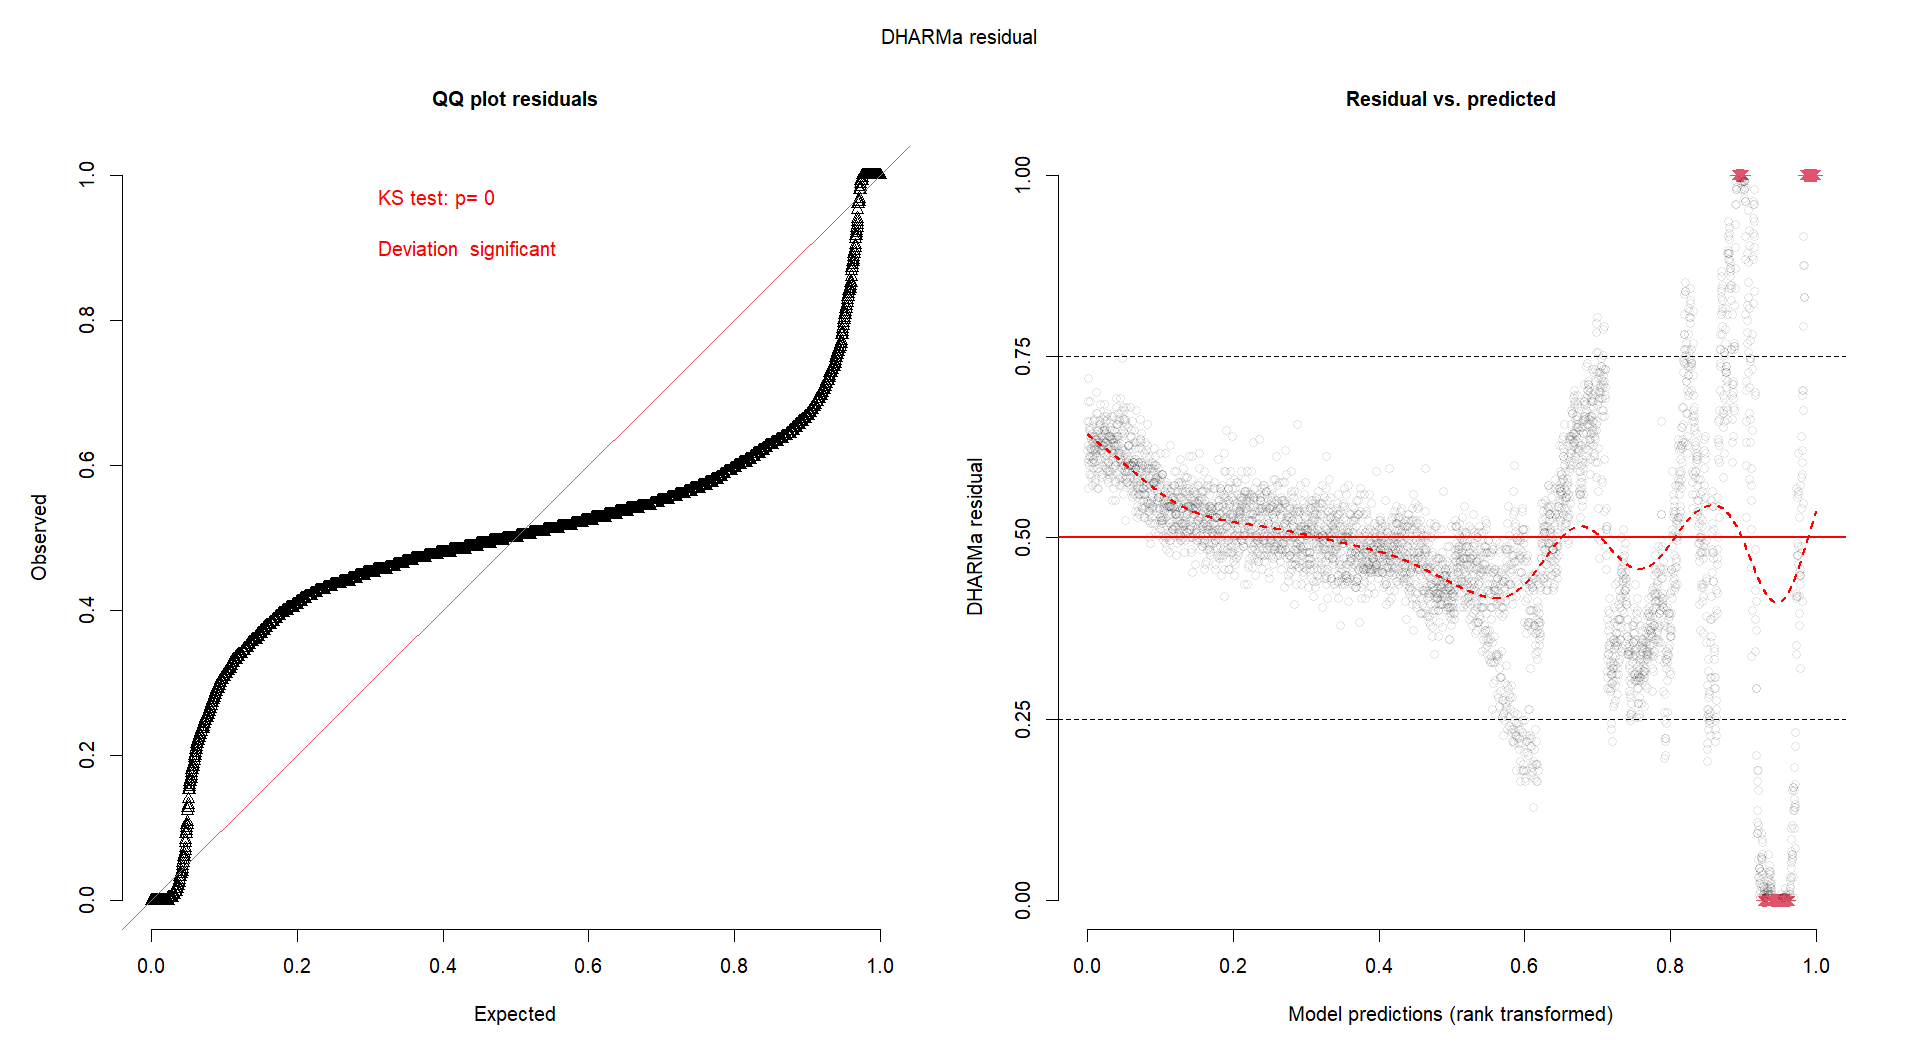
\includegraphics[width=0.9\textwidth]{visuals/DHARMA_gtmb4.png}
    \caption{DHARMA for gtmb4}
    \label{fig:dharmagtmb4}
\end{figure}

% DHARMA for gam4
\begin{figure}[h]
    \centering
    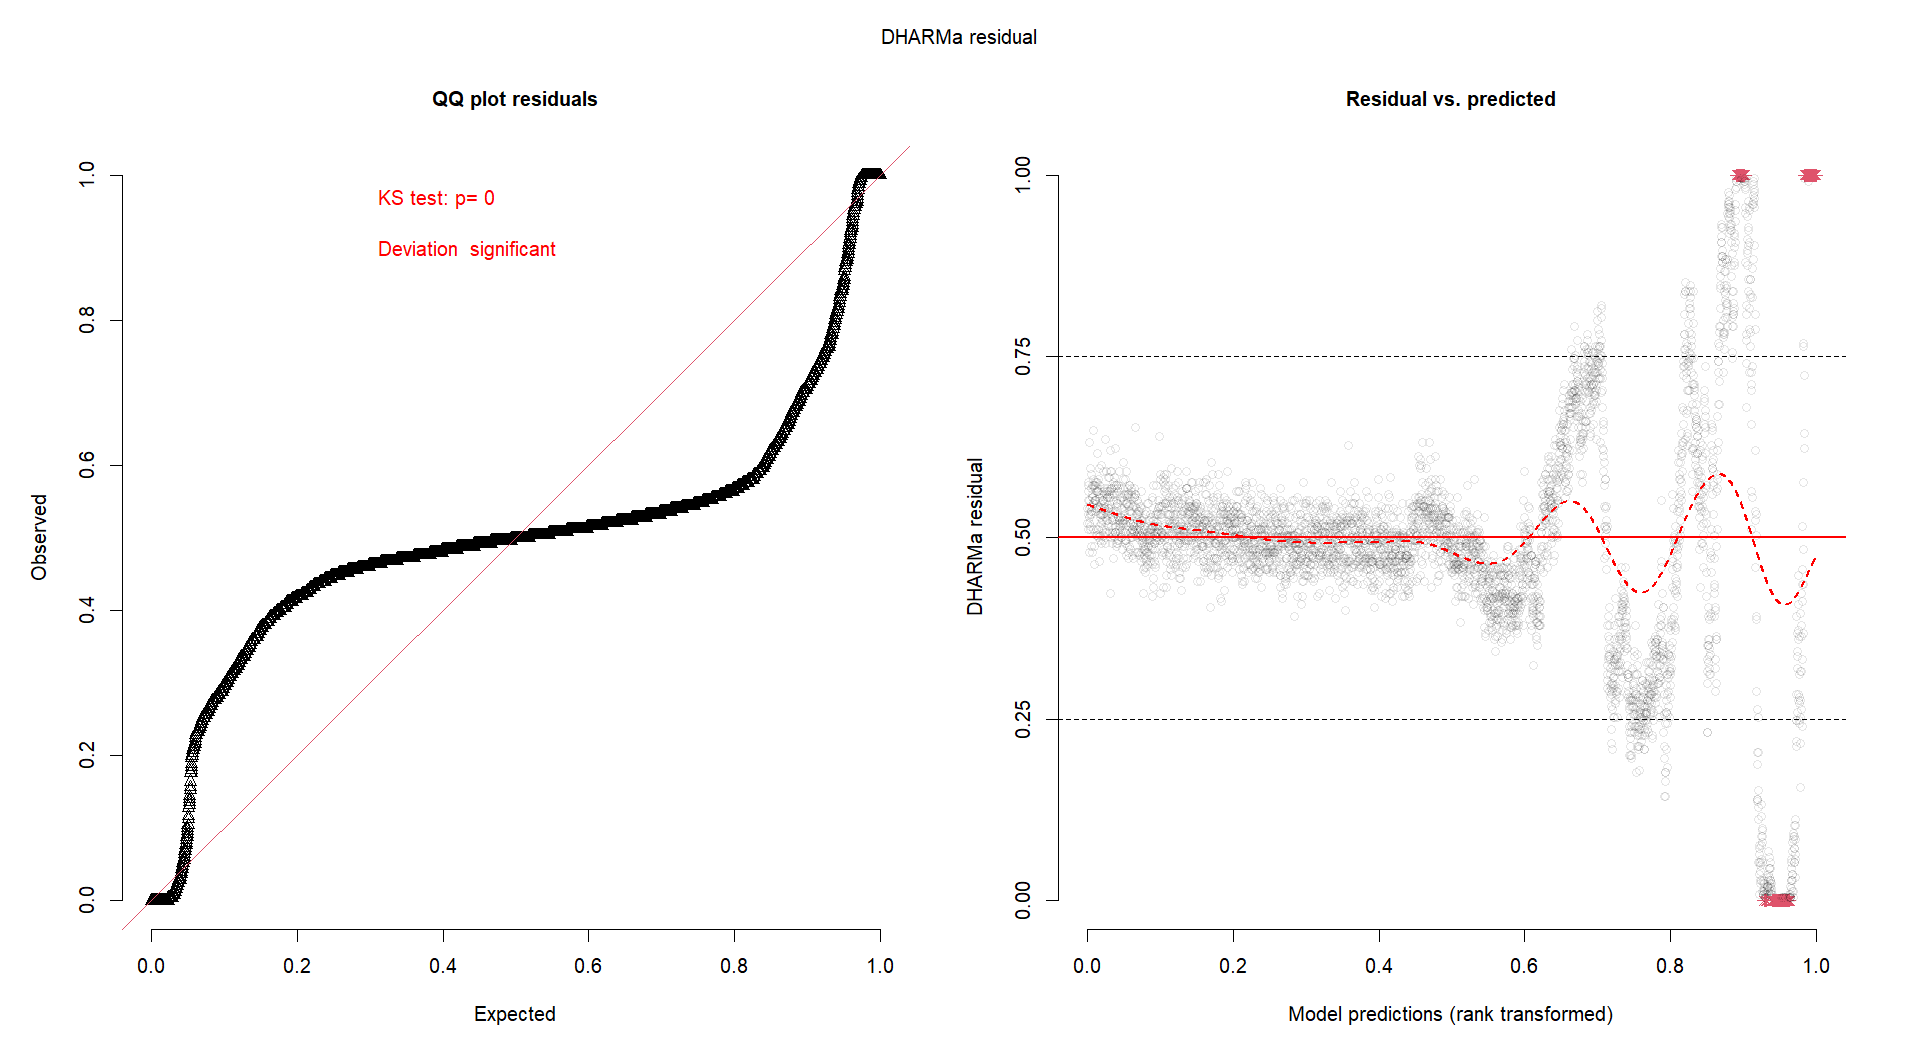
\includegraphics[width=0.9\textwidth]{visuals/DHARMa_gam4.png}
    \caption{DHARMA for gam4}
    \label{fig:dharmagam4}
\end{figure}

% Model Fit for gtmb4
\begin{figure}[h]
    \centering
    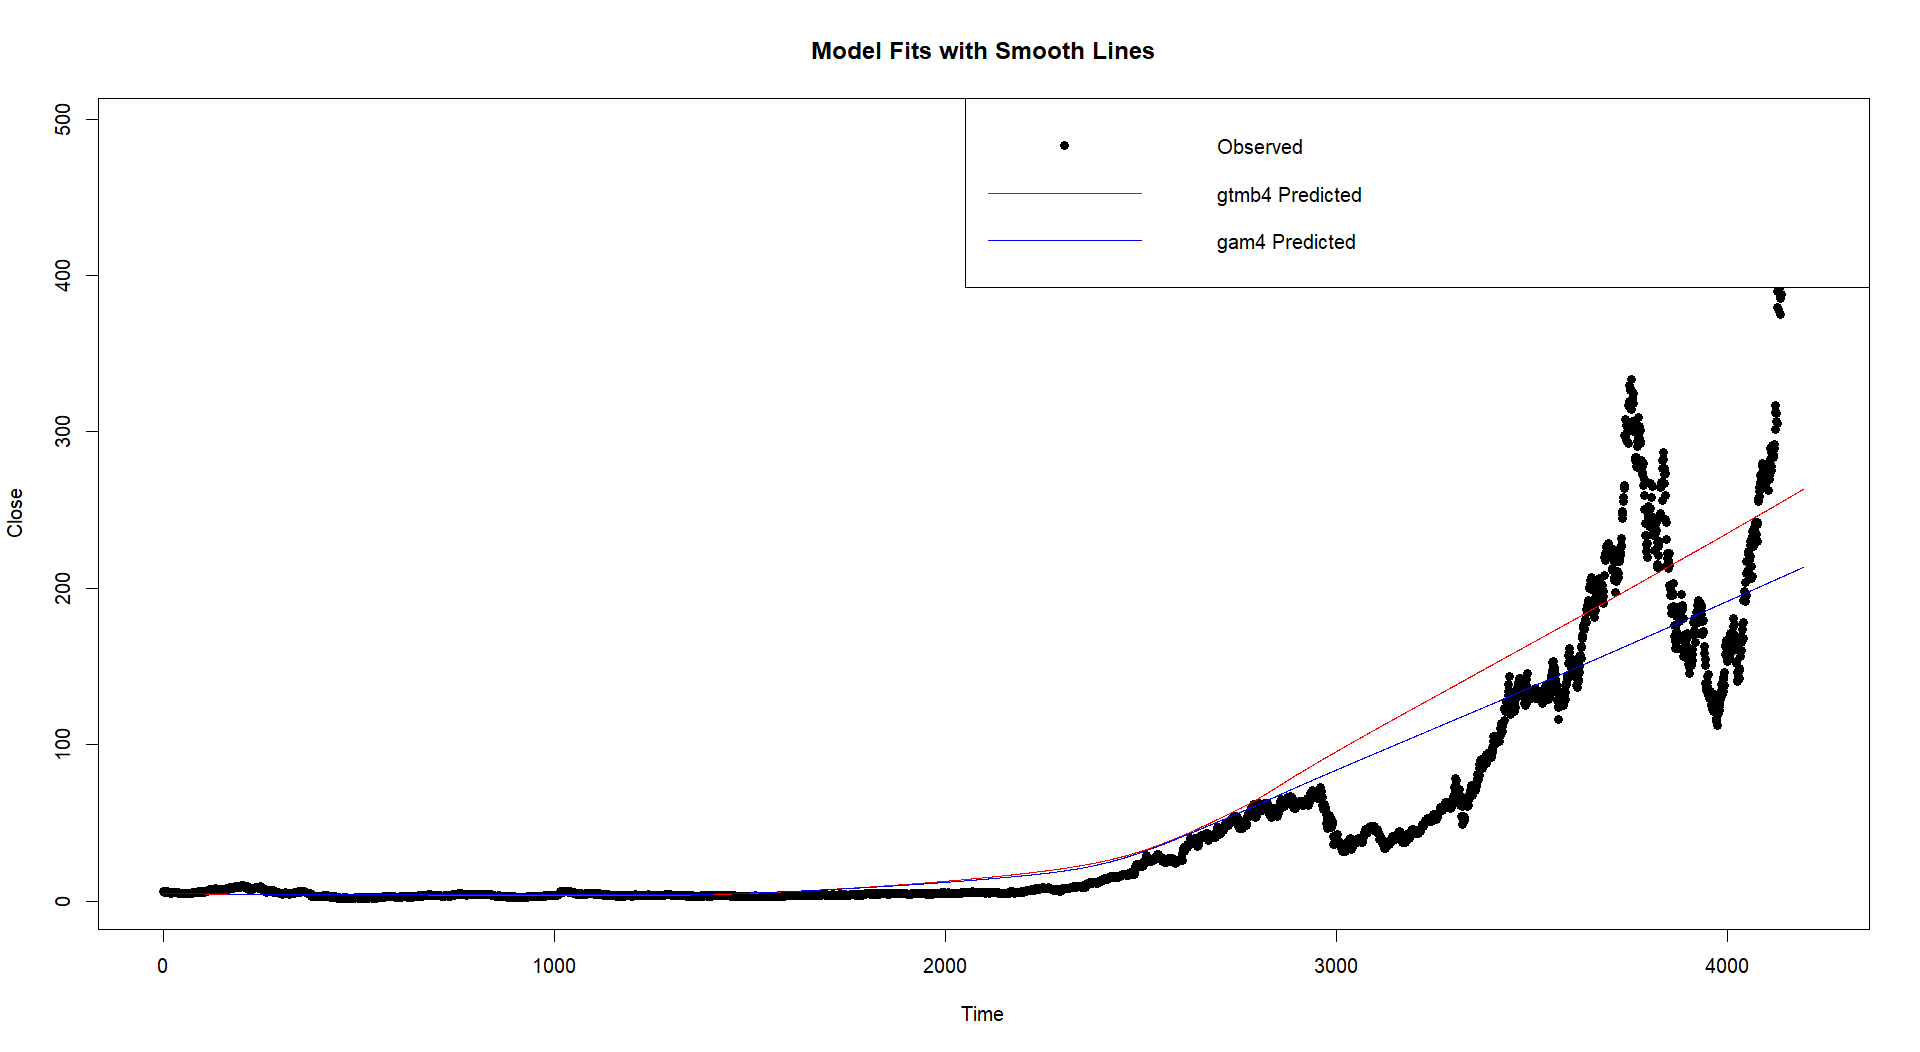
\includegraphics[width=0.9\textwidth]{visuals/mod_fit_gtmb4.png}
    \caption{Model Fit for gtmb4}
    \label{fig:modfitgtmb4}
\end{figure}

% DHARMA for gtmb5
\begin{figure}[h]
    \centering
    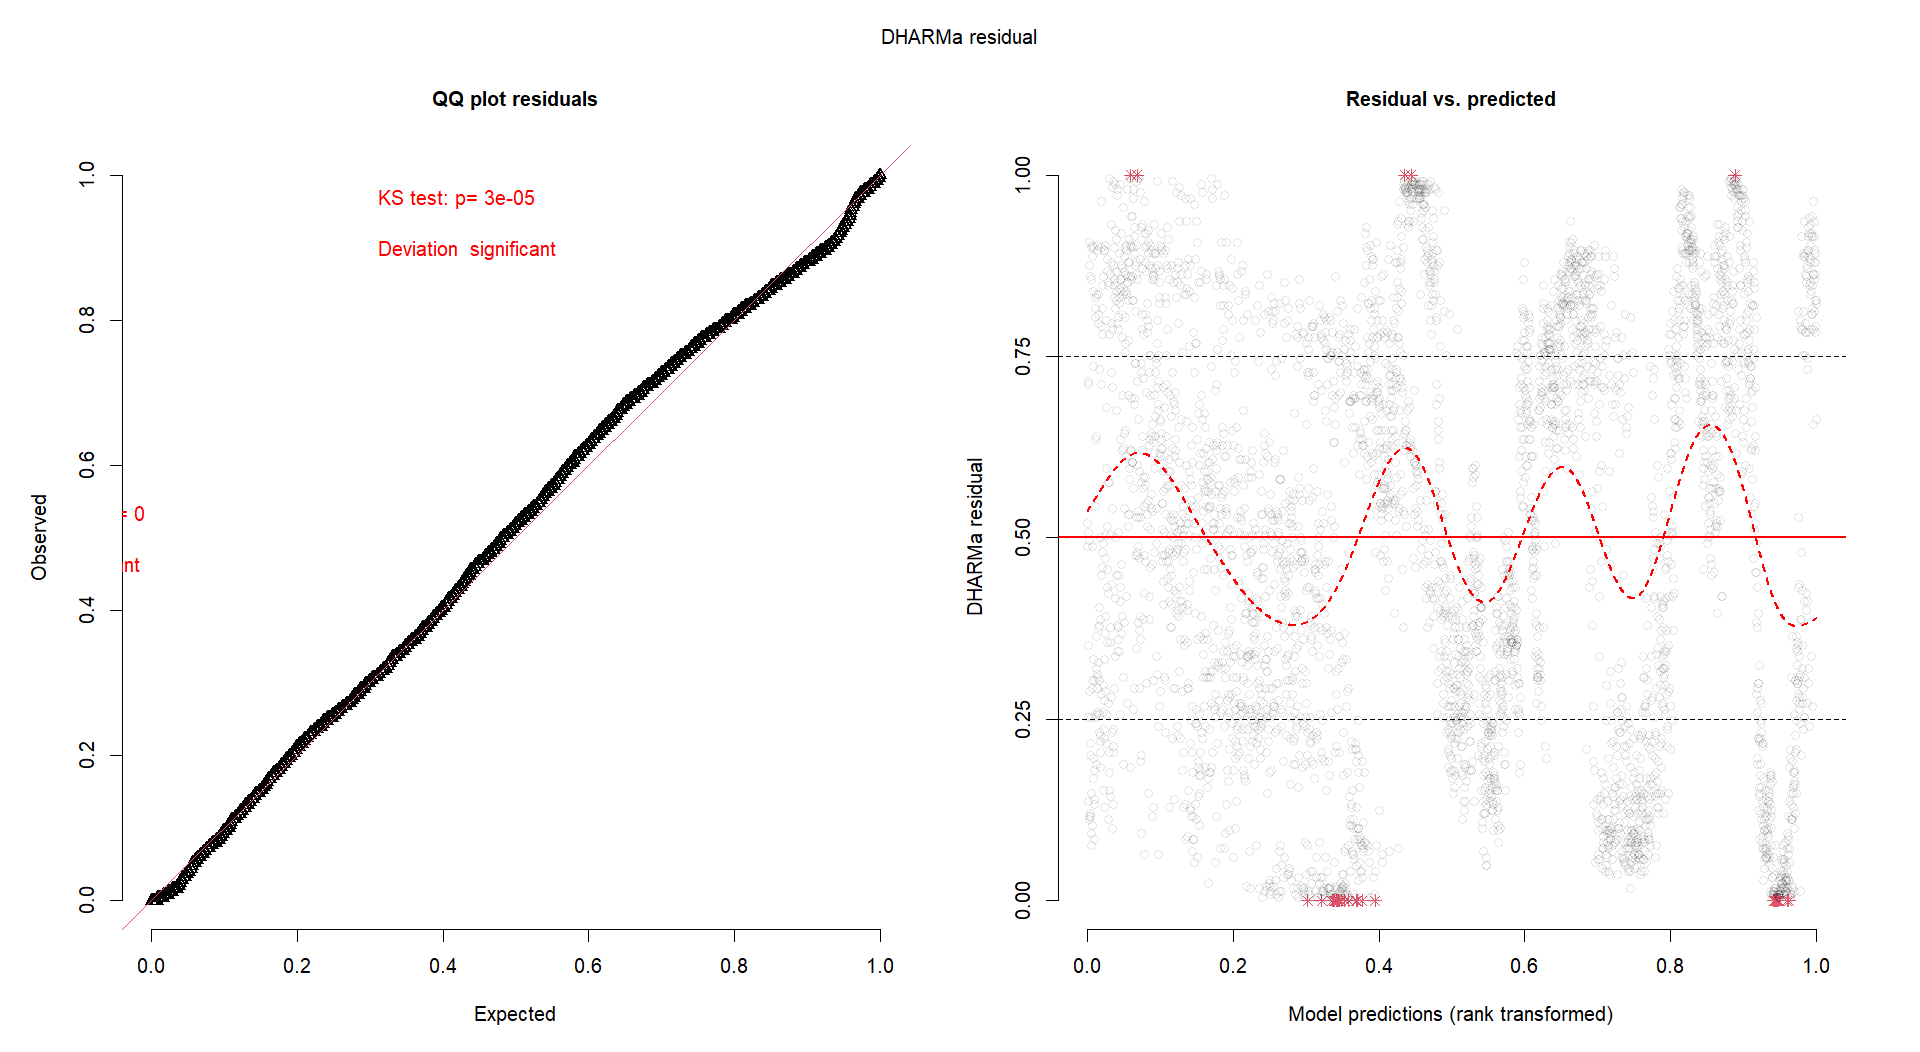
\includegraphics[width=0.9\textwidth]{visuals/DHARMa_gtmb5.png}
    \caption{DHARMA for gtmb5}
    \label{fig:dharmagtmb5}
\end{figure}

% DHARMA for gam5
\begin{figure}[h]
    \centering
    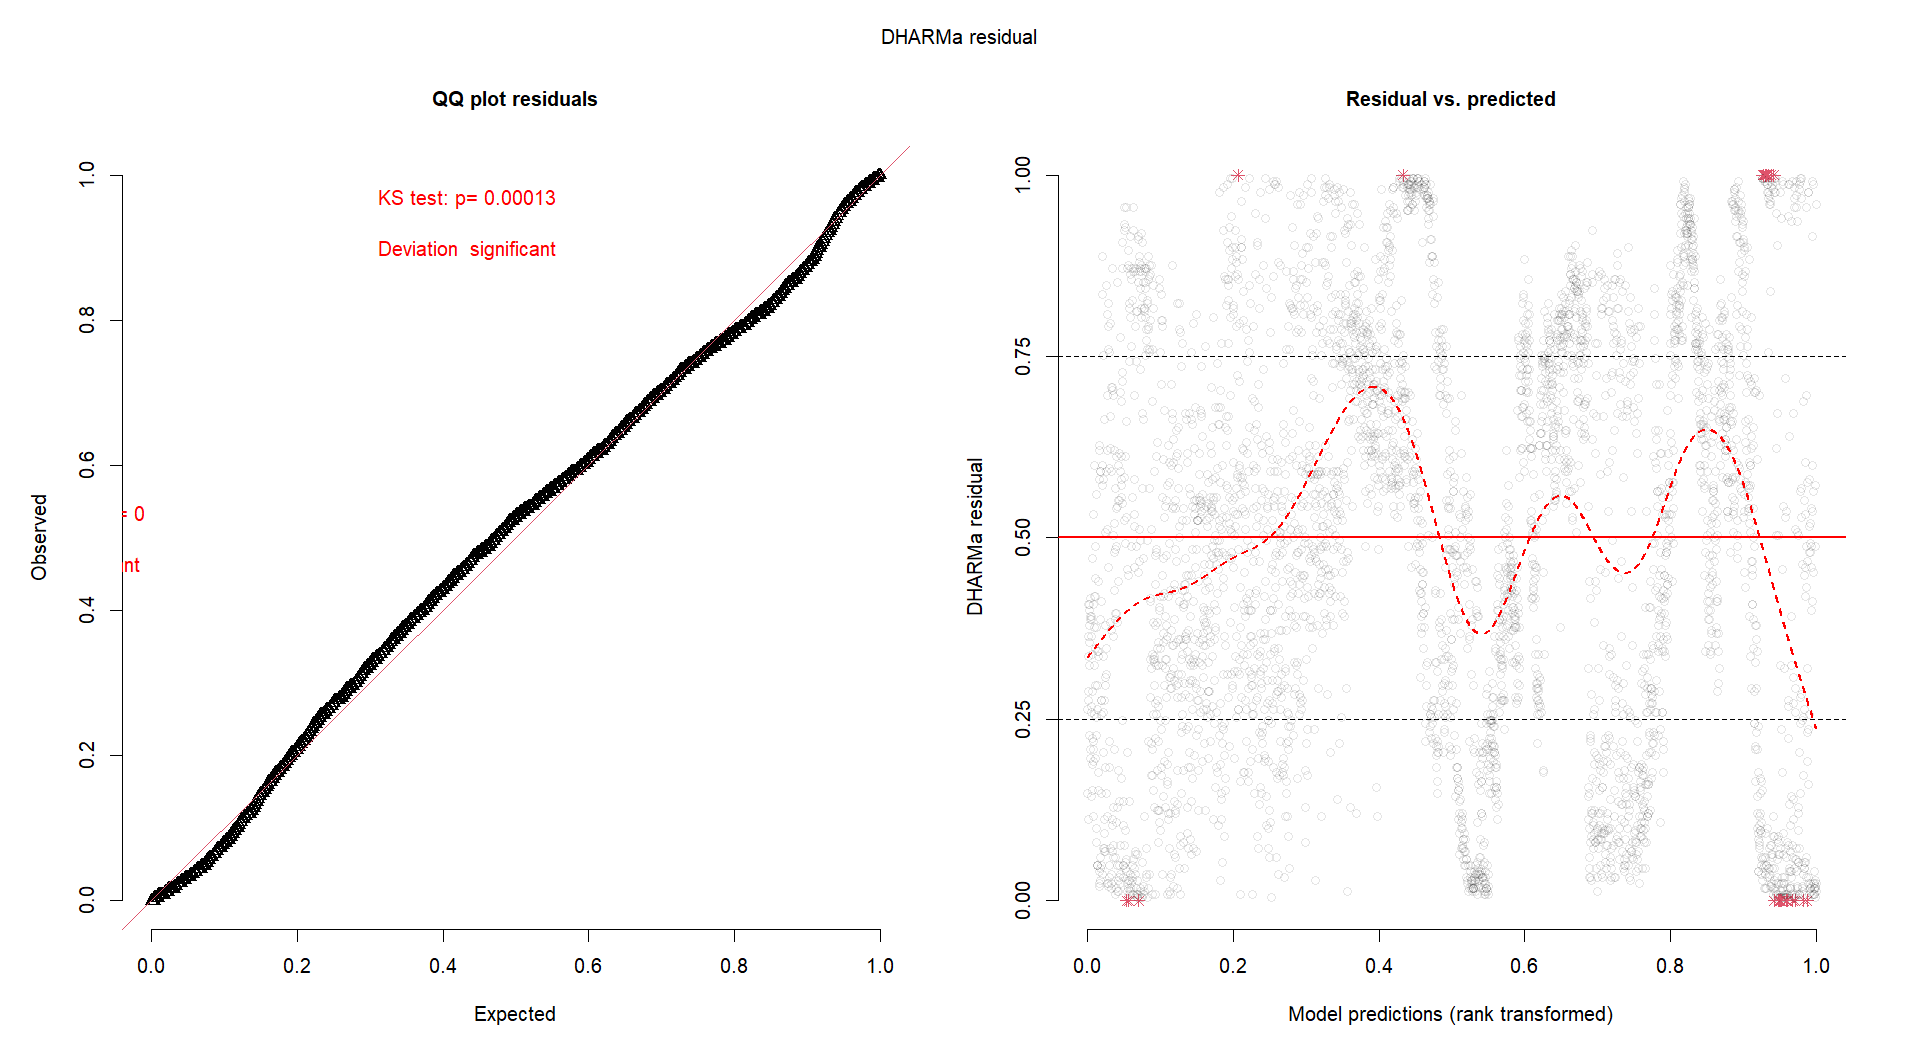
\includegraphics[width=0.9\textwidth]{visuals/DHARMa_gam5.png}
    \caption{DHARMA for gam5}
    \label{fig:dharmagam5}
\end{figure}

% Model Fit for gtmb5
\begin{figure}[h]
    \centering
    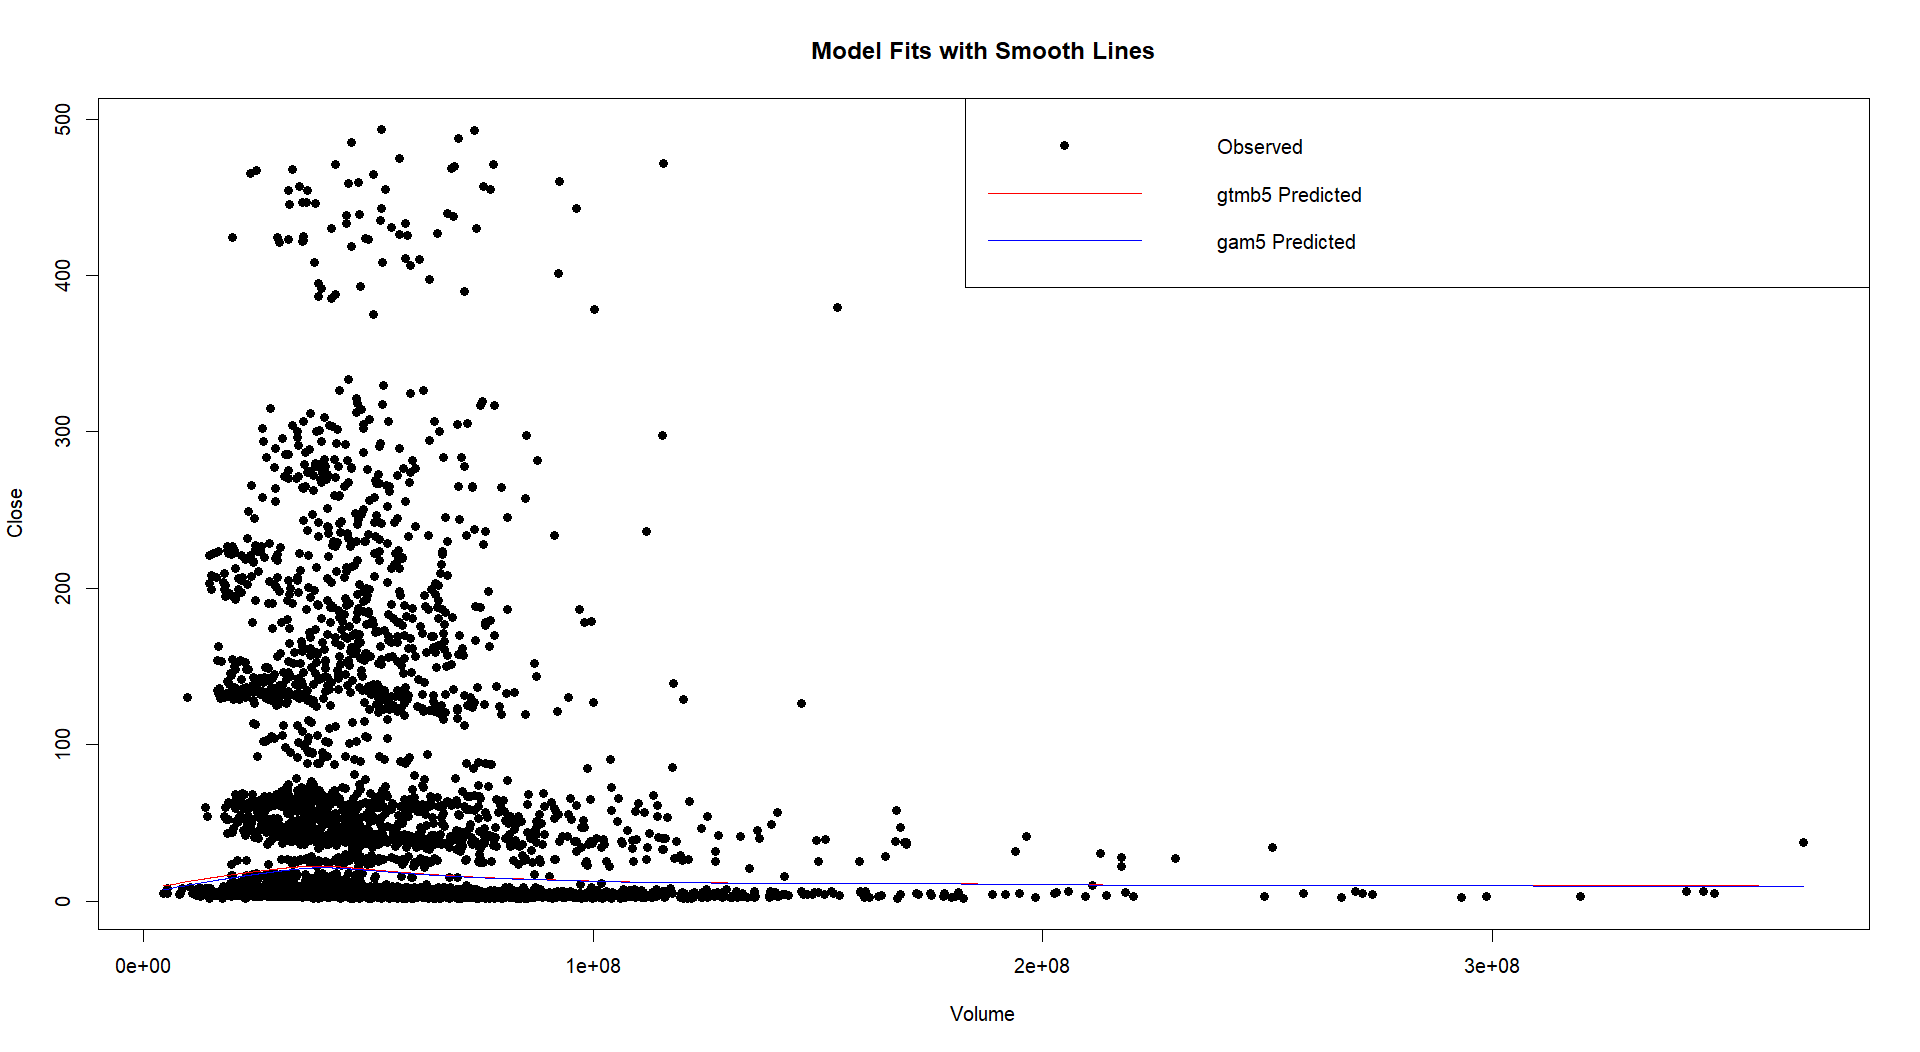
\includegraphics[width=0.9\textwidth]{visuals/model_fit_gtmb5.png}
    \caption{Model Fit for gtmb5}
    \label{fig:modfitgtmb5}
\end{figure}

% DHARMA for gtmb6
\begin{figure}[h]
    \centering
    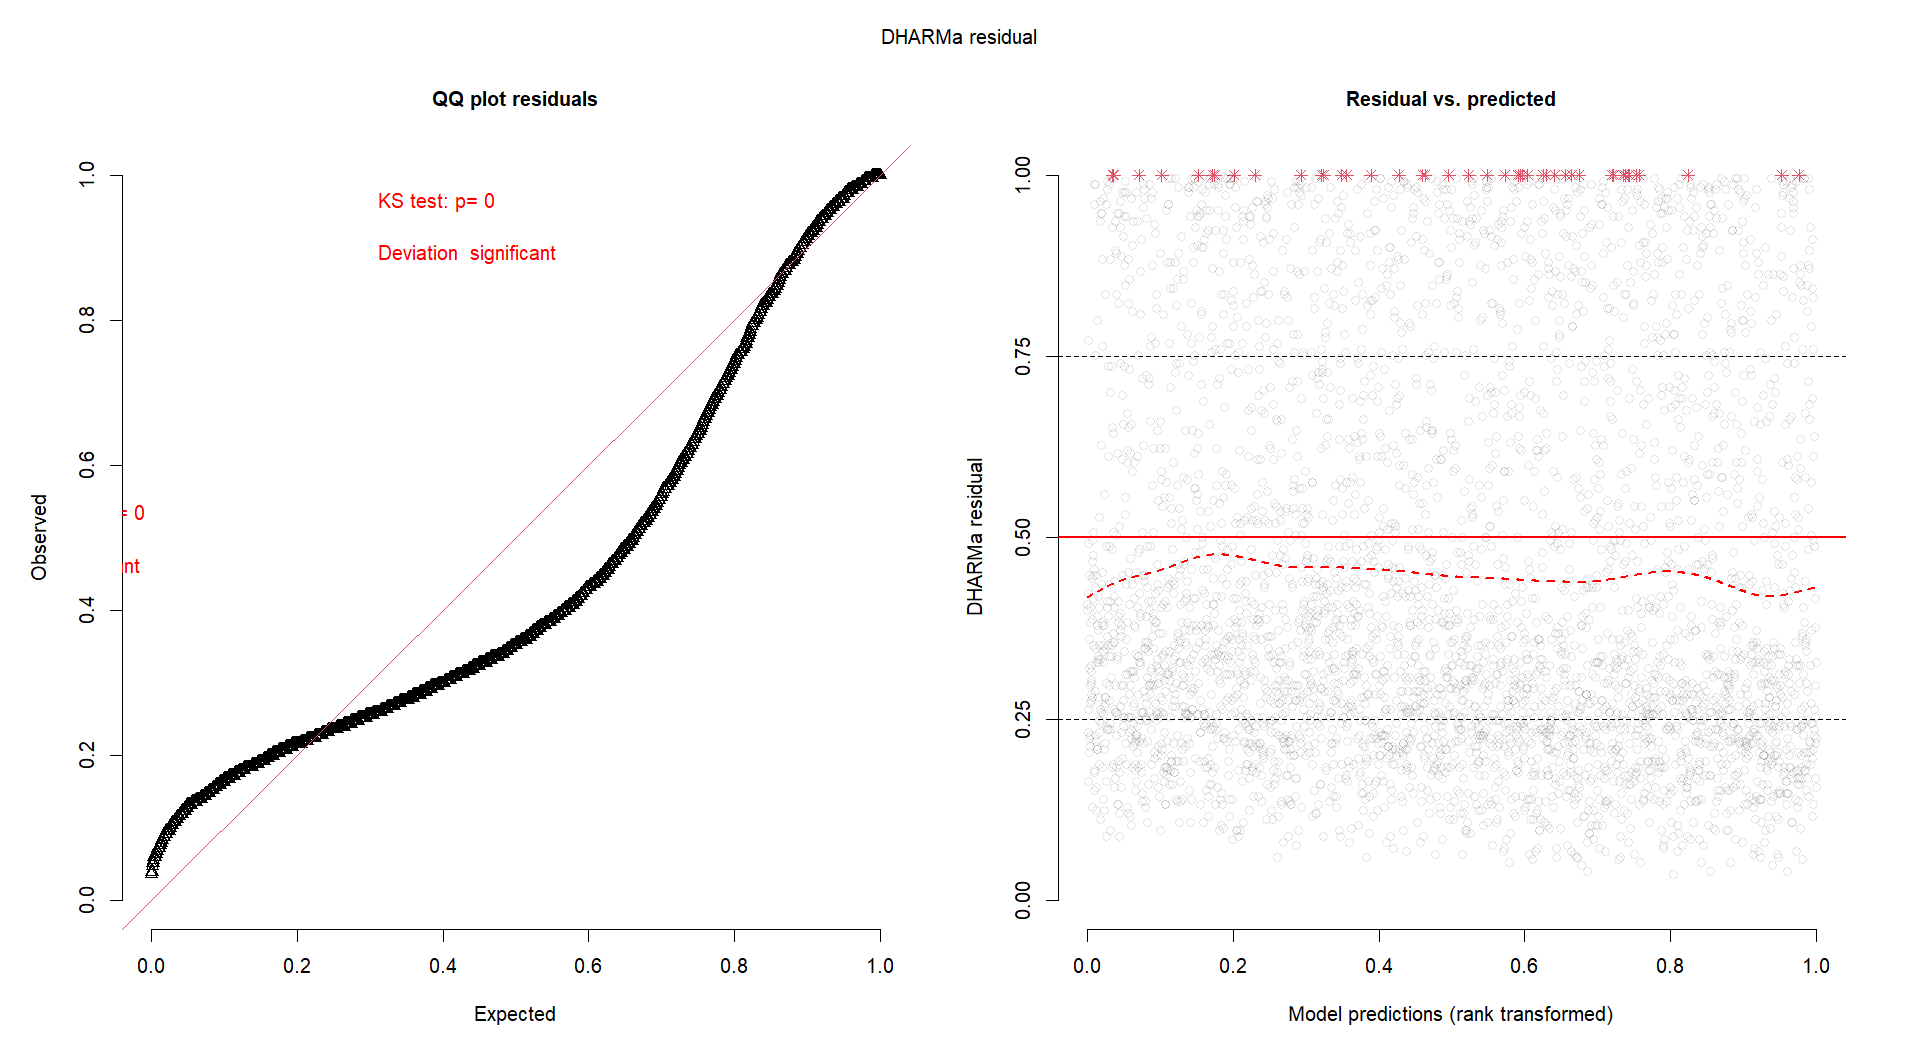
\includegraphics[width=0.9\textwidth]{visuals/DHARMa_gtmb6.png}
    \caption{DHARMA for gtmb6}
    \label{fig:dharmagtmb6}
\end{figure}

% DHARMA for gam6
\begin{figure}[h]
    \centering
    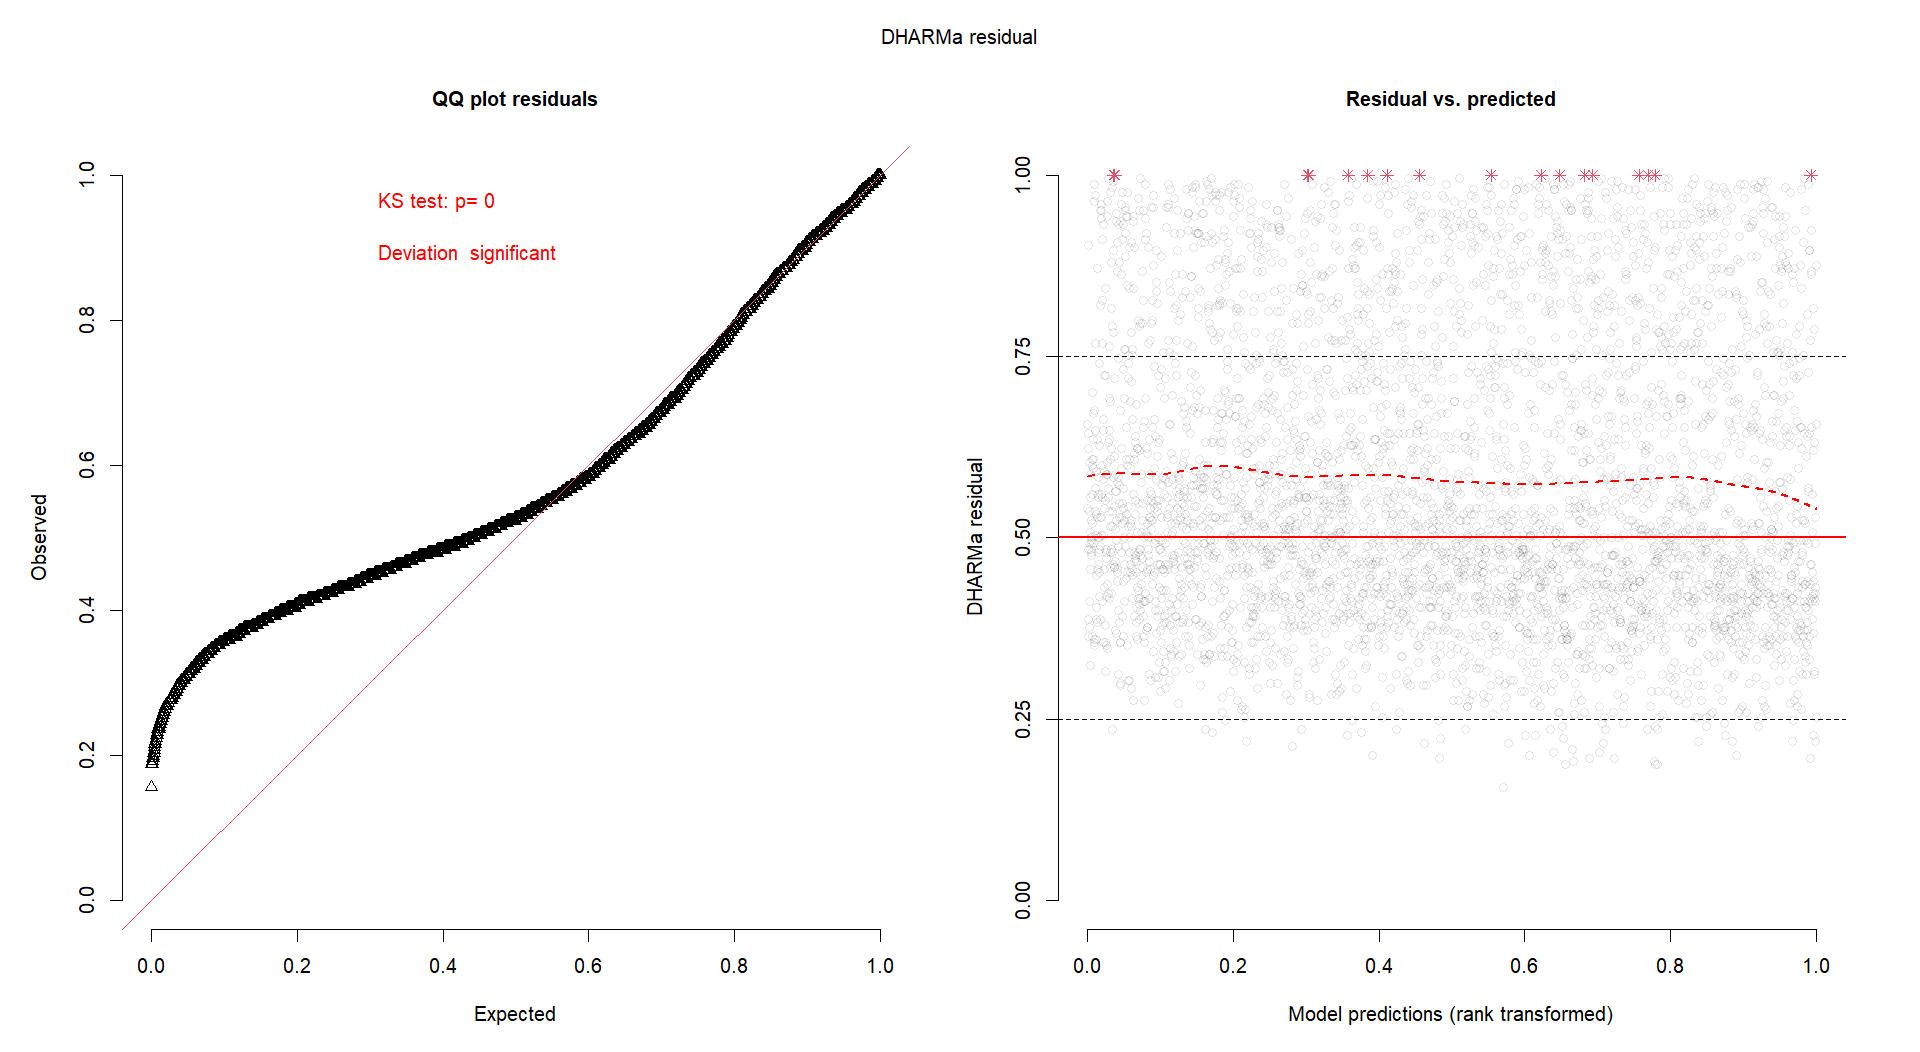
\includegraphics[width=0.9\textwidth]{visuals/DHARMa_gam6.png}
    \caption{DHARMA for gam6}
    \label{fig:dharmagam6}
\end{figure}


% Model Fit for gtmb6
\begin{figure}[h]
    \centering
    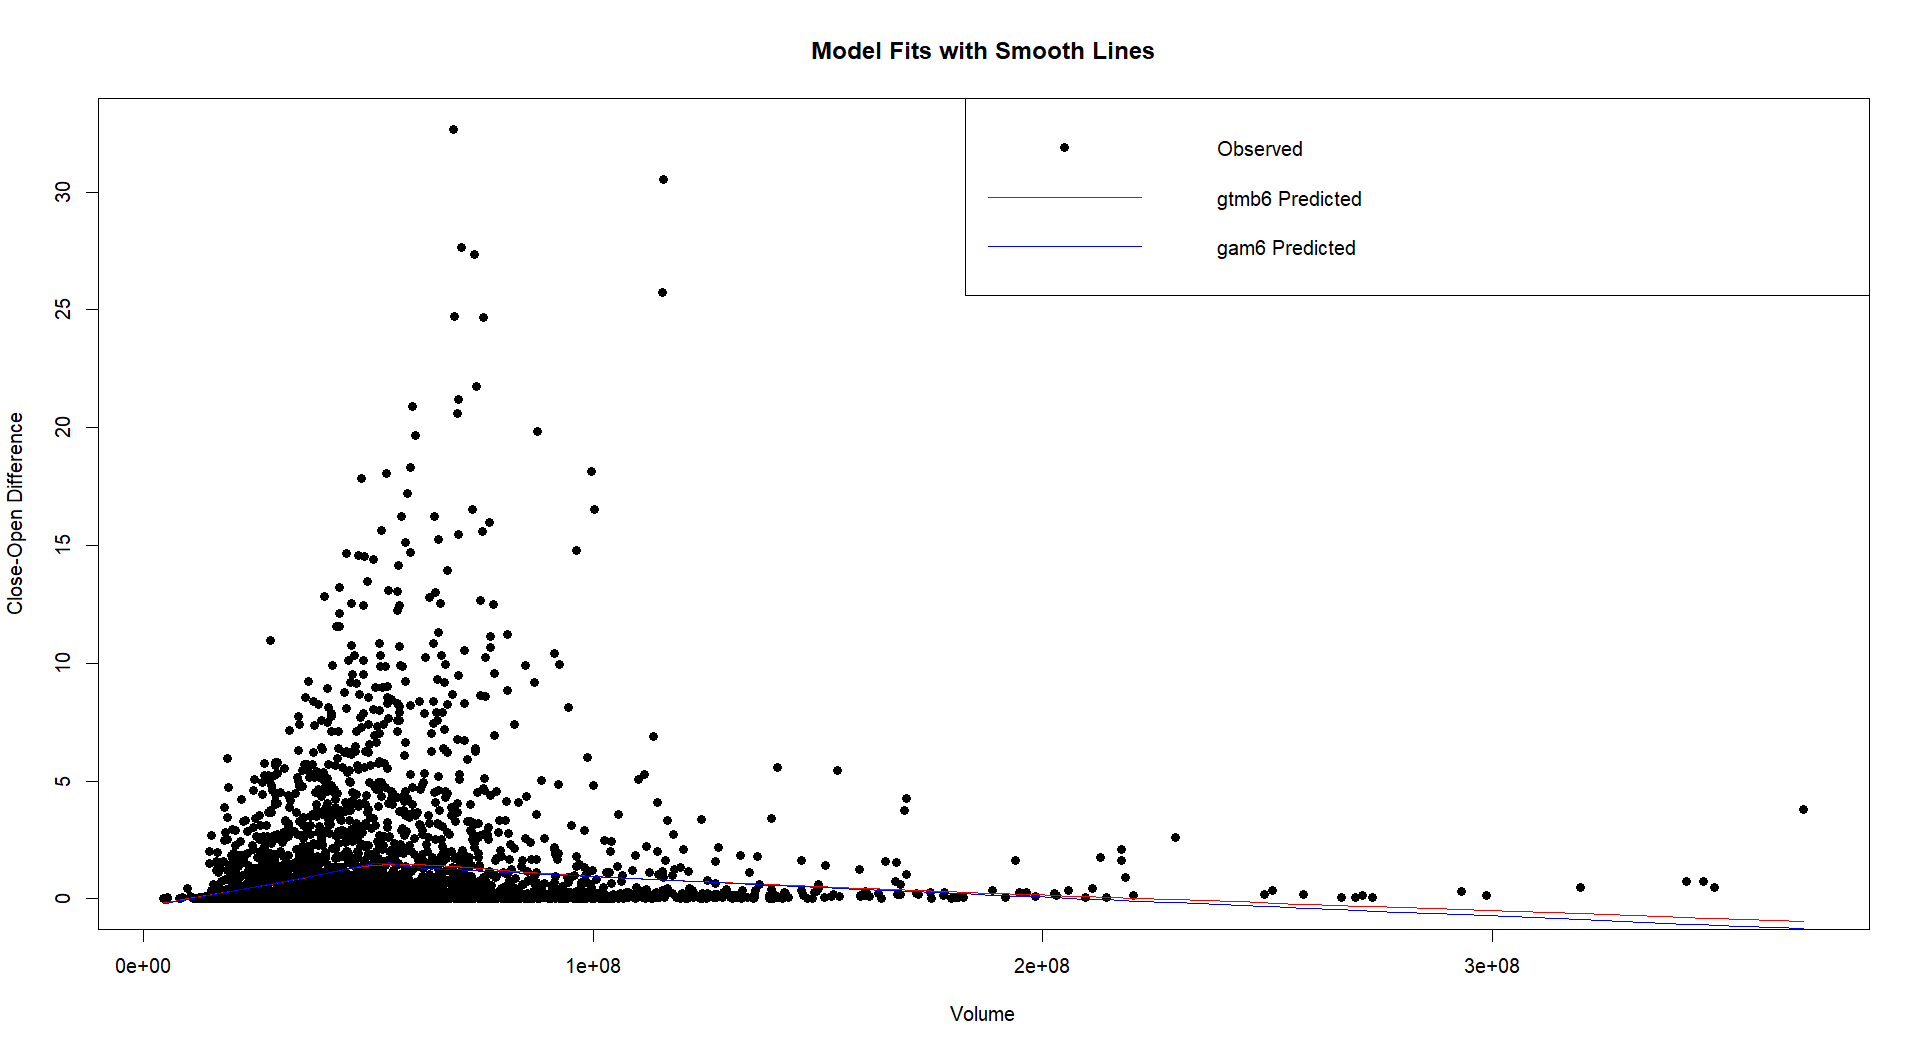
\includegraphics[width=0.9\textwidth]{visuals/model_fit_gtmb6.png}
    \caption{Model Fit for gtmb6}
    \label{fig:modfitgtmb6}
\end{figure}

% DHARMA for gtmb7
\begin{figure}[h]
    \centering
    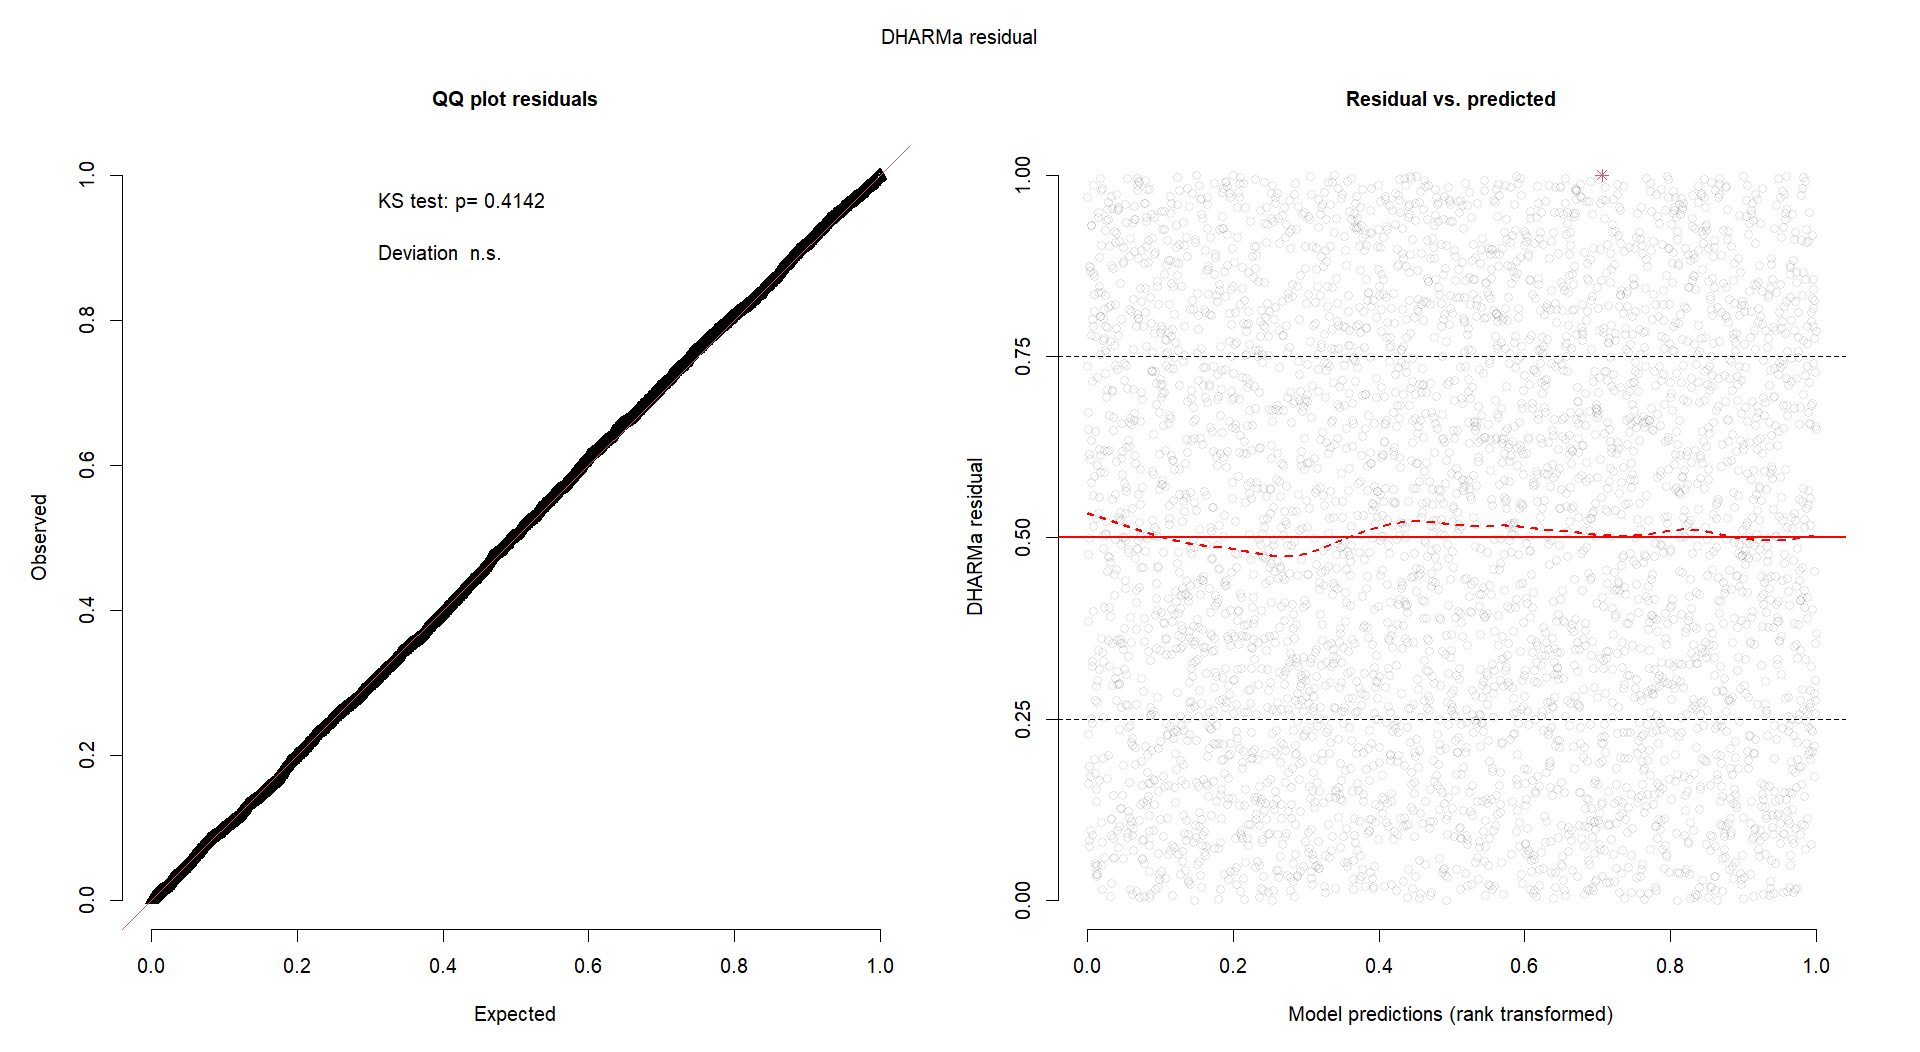
\includegraphics[width=0.9\textwidth]{visuals/DHARMa_gtmb7.png}
    \caption{DHARMA for gtmb7}
    \label{fig:dharmagtmb7}
\end{figure}

% DHARMA for gam7
\begin{figure}[h]
    \centering
    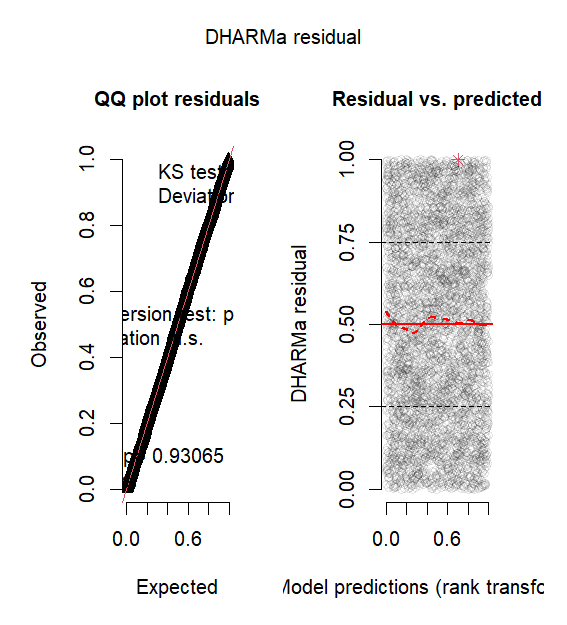
\includegraphics[width=0.9\textwidth]{visuals/DHARMa_gam7.png}
    \caption{DHARMA for gam7}
    \label{fig:dharmagam7}
\end{figure}

% Model Fit for gtmb7
\begin{figure}[h]
    \centering
    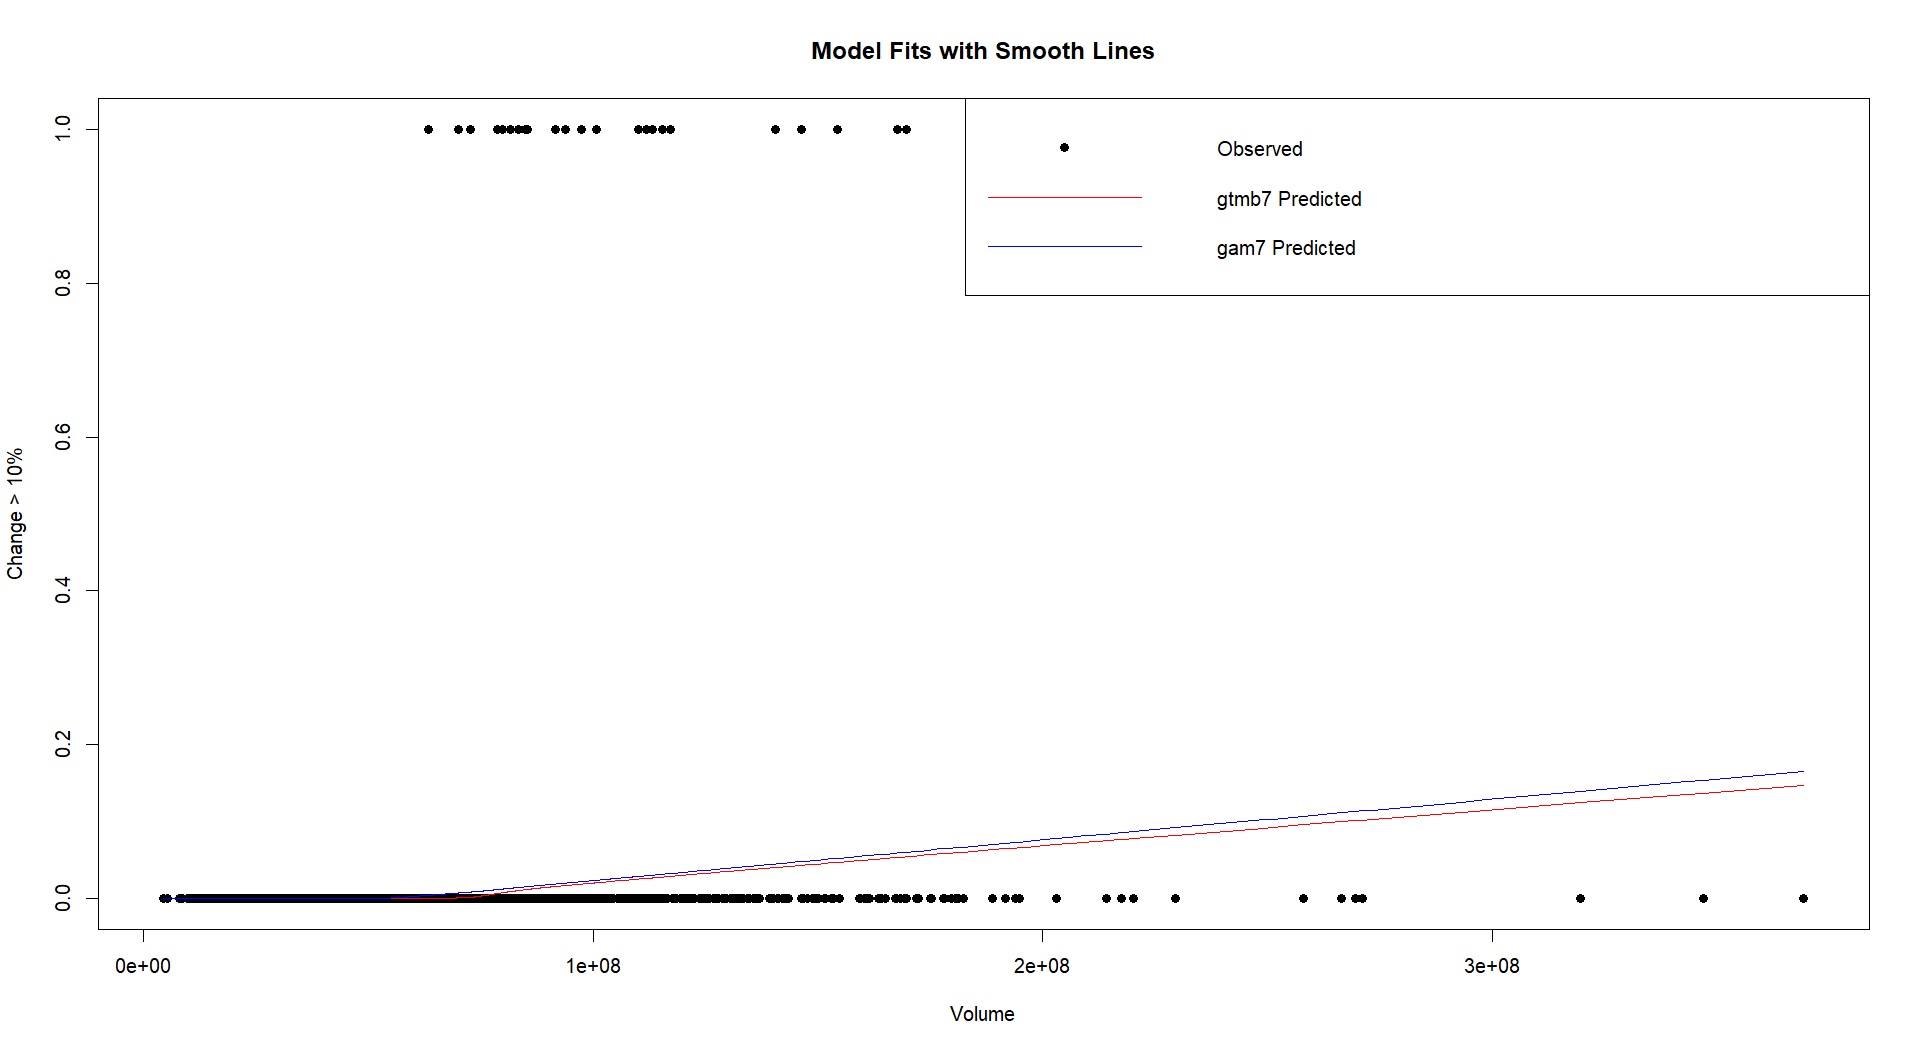
\includegraphics[width=0.9\textwidth]{visuals/model_fit_gtmb7.png}
    \caption{Model Fit for gtmb7}
    \label{fig:modfitgtmb7}
\end{figure}


% Residuals vs Fit for gtmb0s and gtmb0Xr
\begin{figure}[h]
    \centering
    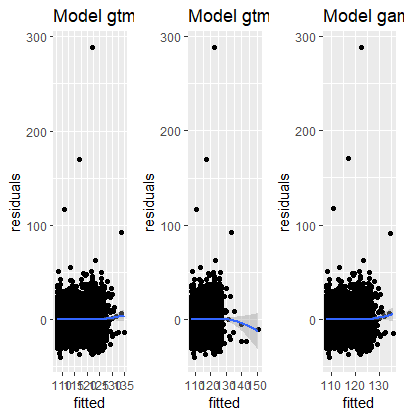
\includegraphics[width=0.9\textwidth]{visuals/ResVSfitgtmb0s.png}
    \caption{Residuals vs Fit for gtmb0s and gtmb0Xr}
    \label{fig:modfitgtmb7}
\end{figure}

% DHARMa for gtmb0s
\begin{figure}[h]
    \centering
    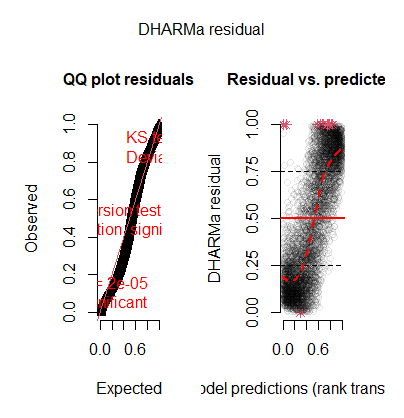
\includegraphics[width=0.9\textwidth]{visuals/DHARMagtmb0s.png}
    \caption{DHARMa for gtmb0s}
    \label{fig:modfitgtmb7}
\end{figure}


% DHARMa for gtmb0Xr
\begin{figure}[h]
    \centering
    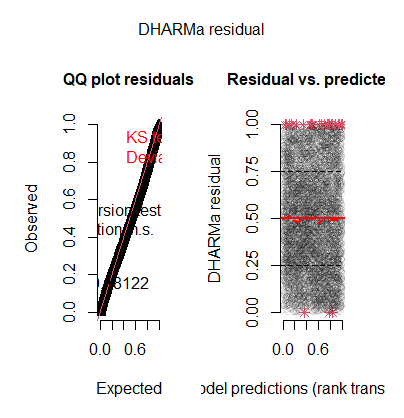
\includegraphics[width=0.9\textwidth]{visuals/DHARMagtmb0Xr.png}
    \caption{DHARMa for gtmb0Xr}
    \label{fig:modfitgtmb7}
\end{figure}

% DHARMa for gtmb1s
\begin{figure}[h]
    \centering
    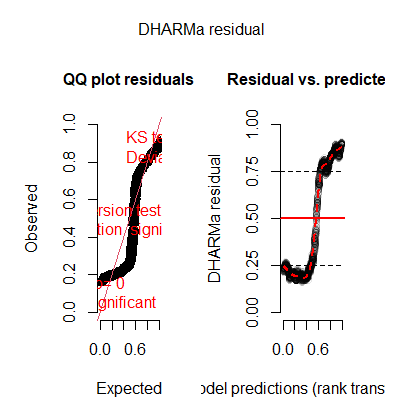
\includegraphics[width=0.9\textwidth]{visuals/DHARMagtmb1s.png}
    \caption{DHARMa for gtmb1s}
    \label{fig:modfitgtmb7}
\end{figure}

% DHARMa for gtmb1Xr
\begin{figure}[h]
    \centering
    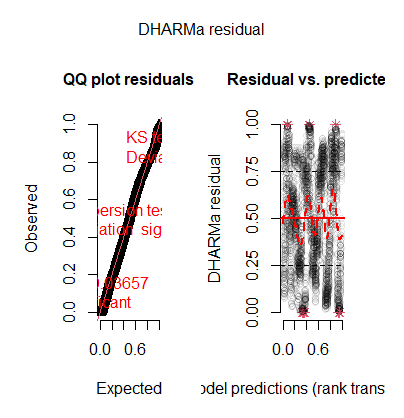
\includegraphics[width=0.9\textwidth]{visuals/DHARMagtmb1Xr.png}
    \caption{DHARMa for gtmb1Xr}
    \label{fig:modfitgtmb7}
\end{figure}


% Model Fit for gtmb1s
\begin{figure}[h]
    \centering
    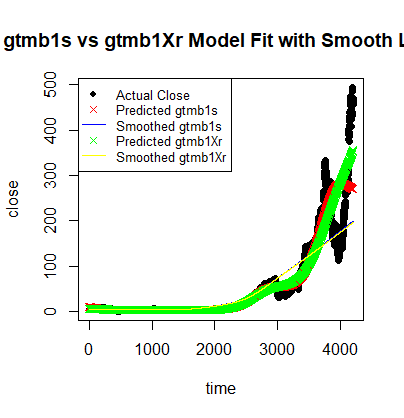
\includegraphics[width=0.9\textwidth]{visuals/ModelFitgtmb1s.png}
    \caption{Model Fit for gtmb1s vs gtmb1Xr}
    \label{fig:modfitgtmb7}
\end{figure}


% Model Fit for gtmb1sk
\begin{figure}[h]
    \centering
    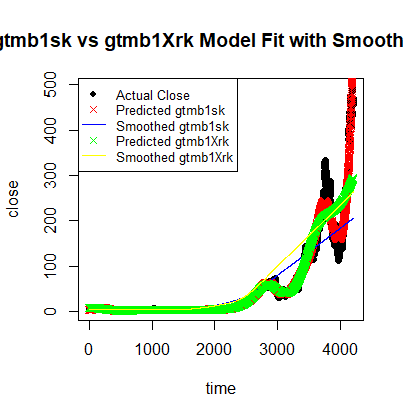
\includegraphics[width=0.9\textwidth]{visuals/ModelFitgtmb1sk.png}
    \caption{Model Fit for gtmb1sk vs gtmb1Xrk, k=20}
    \label{fig:modfitgtmb7}
\end{figure}



% Model Fit for gtmbarimas
\begin{figure}[h]
    \centering
    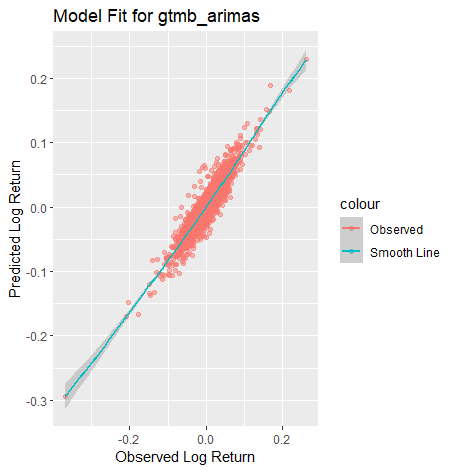
\includegraphics[width=0.9\textwidth]{visuals/ModelFitgtmb_arimas.png}
    \caption{Model Fit for gtmb1arimas}
    \label{fig:modfitgtmb7}
\end{figure}



\newpage